% Template for PLoS
%DIF LATEXDIFF DIFFERENCE FILE
%DIF DEL ./original_submission/wrroc.tex   Tue Jul  9 11:04:57 2024
%DIF ADD wrroc.tex                         Tue Jul  9 10:33:29 2024
% Version 3.6 Aug 2022
%
% % % % % % % % % % % % % % % % % % % % % %
%
% -- IMPORTANT NOTE
%
% This template contains comments intended 
% to minimize problems and delays during our production 
% process. Please follow the template instructions
% whenever possible.
%
% % % % % % % % % % % % % % % % % % % % % % % 
%
% Once your paper is accepted for publica
% PLEASE REMOVE ALL TRACKED CHANGES in this file 
% and leave only the final text of your manuscript. 
% PLOS recommends the use of latexdiff to track changes during review, as this will help to maintain a clean tex file.
% Visit https://www.ctan.org/pkg/latexdiff?lang=en for info or contact us at latex@plos.org.
%
%
% There are no restrictions on package use within the LaTeX files except that no packages listed in the template may be deleted.
%
% Please do not include colors or graphics in the text.
%
% The manuscript LaTeX source should be contained within a single file (do not use \input, \externaldocument, or similar commands).
%
% % % % % % % % % % % % % % % % % % % % % % %
%
% -- FIGURES AND TABLES
%
% Please include tables/figure captions directly after the paragraph where they are first cited in the text.
%
% DO NOT INCLUDE GRAPHICS IN YOUR MANUSCRIPT
% - Figures should be uploaded separately from your manuscript file. 
% - Figures generated using LaTeX should be extracted and removed from the PDF before submission. 
% - Figures containing multiple panels/subfigures must be combined into one image file before submission.
% For figure citations, please use "Fig" instead of "Figure".
% See http://journals.plos.org/plosone/s/figures for PLOS figure guidelines.
%
% Tables should be cell-based and may not contain:
% - spacing/line breaks within cells to alter layout or alignment
% - do not nest tabular environments (no tabular environments within tabular environments)
% - no graphics or colored text (cell background color/shading OK)
% See http://journals.plos.org/plosone/s/tables for table guidelines.
%
% For tables that exceed the width of the text column, use the adjustwidth environment as illustrated in the example table in text below.
%
% % % % % % % % % % % % % % % % % % % % % % % %
%
% -- EQUATIONS, MATH SYMBOLS, SUBSCRIPTS, AND SUPERSCRIPTS
%
% IMPORTANT
% Below are a few tips to help format your equations and other special characters according to our specifications. For more tips to help reduce the possibility of formatting errors during conversion, please see our LaTeX guidelines at http://journals.plos.org/plosone/s/latex
%
% For inline equations, please be sure to include all portions of an equation in the math environment.  For example, x$^2$ is incorrect; this should be formatted as $x^2$ (or $\mathrm{x}^2$ if the romanized font is desired).
%
% Do not include text that is not math in the math environment. For example, CO2 should be written as CO\textsubscript{2} instead of CO$_2$.
%
% Please add line breaks to long display equations when possible in order to fit size of the column. 
%
% For inline equations, please do not include punctuation (commas, etc) within the math environment unless this is part of the equation.
%
% When adding superscript or subscripts outside of brackets/braces, please group using {}.  For example, change "[U(D,E,\gamma)]^2" to "{[U(D,E,\gamma)]}^2". 
%
% Do not use \cal for caligraphic font.  Instead, use \mathcal{}
%
% % % % % % % % % % % % % % % % % % % % % % % % 
%
% Please contact latex@plos.org with any questions.
%
% % % % % % % % % % % % % % % % % % % % % % % %

\documentclass[10pt,letterpaper]{article}
\usepackage[top=0.85in,left=2.75in,footskip=0.75in]{geometry}

% amsmath and amssymb packages, useful for mathematical formulas and symbols
\usepackage{amsmath,amssymb}

% Use adjustwidth environment to exceed column width (see example table in text)
\usepackage{changepage}

% textcomp package and marvosym package for additional characters
\usepackage{textcomp,marvosym}

% cite package, to clean up citations in the main text. Do not remove.
\usepackage{cite}
%% Let's match PeerJ Style:
%\renewcommand\citepunct{; }
%\renewcommand\citeleft{(}
%\renewcommand\citeright{)}
%\renewcommand\citemid{, }

% Use nameref to cite supporting information files (see Supporting Information section for more info)
\usepackage{nameref,hyperref}

% line numbers
\usepackage[right]{lineno}

% ligatures disabled
\usepackage[nopatch=eqnum]{microtype}
\DisableLigatures[f]{encoding = *, family = * }

% color can be used to apply background shading to table cells only
\usepackage[table]{xcolor}
\hypersetup{
    colorlinks,
    linkcolor={red!50!black},
    citecolor={blue!50!black},
    urlcolor={blue!80!black}
}

% array package and thick rules for tables
\usepackage{array}

% create "+" rule type for thick vertical lines
\newcolumntype{+}{!{\vrule width 2pt}}

% create \thickcline for thick horizontal lines of variable length
\newlength\savedwidth
\newcommand\thickcline[1]{%
  \noalign{\global\savedwidth\arrayrulewidth\global\arrayrulewidth 2pt}%
  \cline{#1}%
  \noalign{\vskip\arrayrulewidth}%
  \noalign{\global\arrayrulewidth\savedwidth}%
}

% \thickhline command for thick horizontal lines that span the table
\newcommand\thickhline{\noalign{\global\savedwidth\arrayrulewidth\global\arrayrulewidth 2pt}%
\hline
\noalign{\global\arrayrulewidth\savedwidth}}


% Remove comment for double spacing
%\usepackage{setspace} 
%\doublespacing

% Text layout
\raggedright
\setlength{\parindent}{0.5cm}
\textwidth 5.25in 
\textheight 8.75in

% Bold the 'Figure #' in the caption and separate it from the title/caption with a period
% Captions will be left justified
\usepackage[aboveskip=1pt,labelfont=bf,labelsep=period,justification=raggedright,singlelinecheck=off]{caption}
\renewcommand{\figurename}{Fig}


% Use the PLoS provided BiBTeX style
\bibliographystyle{plos2015}

% Remove brackets from numbering in List of References
\makeatletter
\renewcommand{\@biblabel}[1]{\quad#1.}
\makeatother

%DIF 158a158
\usepackage{listings} %DIF > 
%DIF -------

%DIF 159d160
%DIF < 
%DIF -------
% Header and Footer with logo
\usepackage{lastpage,fancyhdr,graphicx}
\usepackage{epstopdf}
%\pagestyle{myheadings}
\pagestyle{fancy}
\fancyhf{}
%\setlength{\headheight}{27.023pt}
%\lhead{\includegraphics[width=2.0in]{PLOS-submission.eps}}
\rfoot{\thepage/\pageref{LastPage}}
\renewcommand{\headrulewidth}{0pt}
\renewcommand{\footrule}{\hrule height 2pt \vspace{2mm}}
\fancyheadoffset[L]{2.25in}
\fancyfootoffset[L]{2.25in}
\lfoot{\today}

%% Include all macros below

%DIF 177a177-181
\usepackage[inline]{enumitem} %DIF > 
 %DIF > 
\newlist{inlineenum}{enumerate*}{1} %DIF > 
\setlist[inlineenum]{label=\roman*)} %DIF > 
 %DIF > 
%DIF -------
\newcommand{\lorem}{{\bf LOREM}}
\newcommand{\ipsum}{{\bf IPSUM}}
%DIF 179a184-190
 %DIF > 
 %DIF > 
% Macros to insert prefixed terms as hypterlinks %DIF > 
\newcommand{\termsorg}[1]{\href{https://schema.org/#1}{\color{black}{\emph{s:#1}}}} %DIF > 
\newcommand{\termbioschemas}[1]{\href{https://bioschemas.org/#1}{\color{black}{\emph{bioschemas:#1}}}} %DIF > 
\newcommand{\termbsp}[1]{\href{https://bioschemas.org/properties/#1}{\color{black}{\emph{bsp:#1}}}} %DIF > 
\newcommand{\termwfrun}[1]{\href{https://w3id.org/ro/terms/workflow-run\##1}{\color{black}{\emph{wfrun:#1}}}} %DIF > 
%DIF -------

%% END MACROS SECTION
%DIF PREAMBLE EXTENSION ADDED BY LATEXDIFF
%DIF UNDERLINE PREAMBLE %DIF PREAMBLE
\RequirePackage[normalem]{ulem} %DIF PREAMBLE
\RequirePackage{color}\definecolor{RED}{rgb}{1,0,0}\definecolor{BLUE}{rgb}{0,0,1} %DIF PREAMBLE
\providecommand{\DIFaddtex}[1]{{\protect\color{blue}\uwave{#1}}} %DIF PREAMBLE
\providecommand{\DIFdeltex}[1]{{\protect\color{red}\sout{#1}}}                      %DIF PREAMBLE
%DIF SAFE PREAMBLE %DIF PREAMBLE
\providecommand{\DIFaddbegin}{} %DIF PREAMBLE
\providecommand{\DIFaddend}{} %DIF PREAMBLE
\providecommand{\DIFdelbegin}{} %DIF PREAMBLE
\providecommand{\DIFdelend}{} %DIF PREAMBLE
\providecommand{\DIFmodbegin}{} %DIF PREAMBLE
\providecommand{\DIFmodend}{} %DIF PREAMBLE
%DIF FLOATSAFE PREAMBLE %DIF PREAMBLE
\providecommand{\DIFaddFL}[1]{\DIFadd{#1}} %DIF PREAMBLE
\providecommand{\DIFdelFL}[1]{\DIFdel{#1}} %DIF PREAMBLE
\providecommand{\DIFaddbeginFL}{} %DIF PREAMBLE
\providecommand{\DIFaddendFL}{} %DIF PREAMBLE
\providecommand{\DIFdelbeginFL}{} %DIF PREAMBLE
\providecommand{\DIFdelendFL}{} %DIF PREAMBLE
%DIF HYPERREF PREAMBLE %DIF PREAMBLE
\providecommand{\DIFadd}[1]{\texorpdfstring{\DIFaddtex{#1}}{#1}} %DIF PREAMBLE
\providecommand{\DIFdel}[1]{\texorpdfstring{\DIFdeltex{#1}}{}} %DIF PREAMBLE
\newcommand{\DIFscaledelfig}{0.5}
%DIF HIGHLIGHTGRAPHICS PREAMBLE %DIF PREAMBLE
\RequirePackage{settobox} %DIF PREAMBLE
\RequirePackage{letltxmacro} %DIF PREAMBLE
\newsavebox{\DIFdelgraphicsbox} %DIF PREAMBLE
\newlength{\DIFdelgraphicswidth} %DIF PREAMBLE
\newlength{\DIFdelgraphicsheight} %DIF PREAMBLE
% store original definition of \includegraphics %DIF PREAMBLE
\LetLtxMacro{\DIFOincludegraphics}{\includegraphics} %DIF PREAMBLE
\newcommand{\DIFaddincludegraphics}[2][]{{\color{blue}\fbox{\DIFOincludegraphics[#1]{#2}}}} %DIF PREAMBLE
\newcommand{\DIFdelincludegraphics}[2][]{% %DIF PREAMBLE
\sbox{\DIFdelgraphicsbox}{\DIFOincludegraphics[#1]{#2}}% %DIF PREAMBLE
\settoboxwidth{\DIFdelgraphicswidth}{\DIFdelgraphicsbox} %DIF PREAMBLE
\settoboxtotalheight{\DIFdelgraphicsheight}{\DIFdelgraphicsbox} %DIF PREAMBLE
\scalebox{\DIFscaledelfig}{% %DIF PREAMBLE
\parbox[b]{\DIFdelgraphicswidth}{\usebox{\DIFdelgraphicsbox}\\[-\baselineskip] \rule{\DIFdelgraphicswidth}{0em}}\llap{\resizebox{\DIFdelgraphicswidth}{\DIFdelgraphicsheight}{% %DIF PREAMBLE
\setlength{\unitlength}{\DIFdelgraphicswidth}% %DIF PREAMBLE
\begin{picture}(1,1)% %DIF PREAMBLE
\thicklines\linethickness{2pt} %DIF PREAMBLE
{\color[rgb]{1,0,0}\put(0,0){\framebox(1,1){}}}% %DIF PREAMBLE
{\color[rgb]{1,0,0}\put(0,0){\line( 1,1){1}}}% %DIF PREAMBLE
{\color[rgb]{1,0,0}\put(0,1){\line(1,-1){1}}}% %DIF PREAMBLE
\end{picture}% %DIF PREAMBLE
}\hspace*{3pt}}} %DIF PREAMBLE
} %DIF PREAMBLE
\LetLtxMacro{\DIFOaddbegin}{\DIFaddbegin} %DIF PREAMBLE
\LetLtxMacro{\DIFOaddend}{\DIFaddend} %DIF PREAMBLE
\LetLtxMacro{\DIFOdelbegin}{\DIFdelbegin} %DIF PREAMBLE
\LetLtxMacro{\DIFOdelend}{\DIFdelend} %DIF PREAMBLE
\DeclareRobustCommand{\DIFaddbegin}{\DIFOaddbegin \let\includegraphics\DIFaddincludegraphics} %DIF PREAMBLE
\DeclareRobustCommand{\DIFaddend}{\DIFOaddend \let\includegraphics\DIFOincludegraphics} %DIF PREAMBLE
\DeclareRobustCommand{\DIFdelbegin}{\DIFOdelbegin \let\includegraphics\DIFdelincludegraphics} %DIF PREAMBLE
\DeclareRobustCommand{\DIFdelend}{\DIFOaddend \let\includegraphics\DIFOincludegraphics} %DIF PREAMBLE
\LetLtxMacro{\DIFOaddbeginFL}{\DIFaddbeginFL} %DIF PREAMBLE
\LetLtxMacro{\DIFOaddendFL}{\DIFaddendFL} %DIF PREAMBLE
\LetLtxMacro{\DIFOdelbeginFL}{\DIFdelbeginFL} %DIF PREAMBLE
\LetLtxMacro{\DIFOdelendFL}{\DIFdelendFL} %DIF PREAMBLE
\DeclareRobustCommand{\DIFaddbeginFL}{\DIFOaddbeginFL \let\includegraphics\DIFaddincludegraphics} %DIF PREAMBLE
\DeclareRobustCommand{\DIFaddendFL}{\DIFOaddendFL \let\includegraphics\DIFOincludegraphics} %DIF PREAMBLE
\DeclareRobustCommand{\DIFdelbeginFL}{\DIFOdelbeginFL \let\includegraphics\DIFdelincludegraphics} %DIF PREAMBLE
\DeclareRobustCommand{\DIFdelendFL}{\DIFOaddendFL \let\includegraphics\DIFOincludegraphics} %DIF PREAMBLE
%DIF COLORLISTINGS PREAMBLE %DIF PREAMBLE
\RequirePackage{listings} %DIF PREAMBLE
\RequirePackage{color} %DIF PREAMBLE
\lstdefinelanguage{DIFcode}{ %DIF PREAMBLE
%DIF DIFCODE_UNDERLINE %DIF PREAMBLE
  moredelim=[il][\color{red}\sout]{\%DIF\ <\ }, %DIF PREAMBLE
  moredelim=[il][\color{blue}\uwave]{\%DIF\ >\ } %DIF PREAMBLE
} %DIF PREAMBLE
\lstdefinestyle{DIFverbatimstyle}{ %DIF PREAMBLE
	language=DIFcode, %DIF PREAMBLE
	basicstyle=\ttfamily, %DIF PREAMBLE
	columns=fullflexible, %DIF PREAMBLE
	keepspaces=true %DIF PREAMBLE
} %DIF PREAMBLE
\lstnewenvironment{DIFverbatim}{\lstset{style=DIFverbatimstyle}}{} %DIF PREAMBLE
\lstnewenvironment{DIFverbatim*}{\lstset{style=DIFverbatimstyle,showspaces=true}}{} %DIF PREAMBLE
%DIF END PREAMBLE EXTENSION ADDED BY LATEXDIFF

\begin{document}
\vspace*{0.2in}

% Title must be 250 characters or less.
\begin{flushleft}
{\Large
\textbf\newline{Recording provenance of workflow runs with RO-Crate} % Please use "sentence case" for title and headings (capitalize only the first word in a title (or heading), the first word in a subtitle (or subheading), and any proper nouns).
}
\newline
% Insert author names, affiliations and corresponding author email (do not include titles, positions, or degrees).
\\

Simone Leo\textsuperscript{1*},
Michael R. Crusoe\textsuperscript{2,3,4},
Laura Rodríguez-Navas\textsuperscript{5}, 
Raül Sirvent\textsuperscript{5}, 
Alexander Kanitz\textsuperscript{6,7}, 
Paul De Geest\textsuperscript{8}, 
Rudolf Wittner\textsuperscript{9,10,11}, 
Luca Pireddu\textsuperscript{1}, 
Daniel Garijo\textsuperscript{12}, 
José M. Fernández\textsuperscript{5}, 
Iacopo Colonnelli\textsuperscript{13}, 
Matej Gallo\textsuperscript{9}, 
Tazro Ohta\textsuperscript{14,15}, 
Hirotaka Suetake\textsuperscript{16}, 
Salvador Capella-Gutierrez\textsuperscript{5}, 
Renske de Wit\textsuperscript{2}, 
Bruno P. Kinoshita\textsuperscript{5}, 
Stian Soiland-Reyes\textsuperscript{17,18}
\\
\bigskip
\textbf{1} Center for Advanced Studies, Research, and Development in Sardinia (CRS4), Pula (CA), Italy
\\
\textbf{2} Vrije Universiteit Amsterdam, Amsterdam, The Netherlands
\\
\textbf{3} DTL Projects, The Netherlands
\\
\textbf{4} Forschungszentrum Jülich, Germany
\\
\textbf{5} Barcelona Supercomputing Center, Barcelona, Spain
\\
\textbf{6} Biozentrum, University of Basel, Basel, Switzerland
\\
\textbf{7} Swiss Institute of Bioinformatics, Lausanne, Switzerland
\\
\textbf{8} VIB Data Core, Gent, Belgium
\\
\textbf{9} Faculty of Informatics, Masaryk University, Brno, Czech Republic
\\
\textbf{10} Institute of Computer Science, Masaryk University, Brno, Czech Republic
\\
\textbf{11} BBMRI-ERIC, Graz, Austria
\\
\textbf{12} Ontology Engineering Group, Universidad Politécnica de Madrid, Madrid, Spain
\\
\textbf{13} Computer Science \DIFdelbegin \DIFdel{Dept.}\DIFdelend \DIFaddbegin \DIFadd{Department}\DIFaddend , Università degli Studi di Torino, Torino, Italy
\\
\textbf{14} Database Center for Life Science, Joint Support-Center for Data Science Research, Research Organization of Information and Systems, Shizuoka, Japan
\\
\textbf{15} Institute for Advanced Academic Research, Chiba University, Chiba, Japan
\\
\textbf{16} Sator, \DIFdelbegin \DIFdel{Inc.}\DIFdelend \DIFaddbegin \DIFadd{Incorporated}\DIFaddend , Tokyo, Japan
\\
\textbf{17} Department of Computer Science, The University of Manchester, Manchester, United Kingdom
\\
\textbf{18} Informatics Institute, University of Amsterdam, Amsterdam, The Netherlands
\\
\bigskip

% Insert additional author notes using the symbols described below. Insert symbol callouts after author names as necessary.
% 
% Remove or comment out the author notes below if they aren't used.
%
% Primary Equal Contribution Note
%\Yinyang These authors contributed equally to this work.

% Additional Equal Contribution Note
% Also use this double-dagger symbol for special authorship notes, such as senior authorship.
%\ddag These authors also contributed equally to this work.

% Current address notes
%\textcurrency Current Address: Dept/Program/Center, Institution Name, City, State, Country % change symbol to "\textcurrency a" if more than one current address note
% \textcurrency b Insert second current address 
% \textcurrency c Insert third current address

% Deceased author note
%\dag Deceased

% Group/Consortium Author Note
%\textpilcrow Membership list can be found in the Acknowledgments section.

% Use the asterisk to denote corresponding authorship and provide email address in note below.
* simone.leo@crs4.it \DIFaddbegin \DIFadd{(SL)
}\DIFaddend 

\end{flushleft}
% Please keep the abstract below 300 words
\section*{Abstract}
Recording the provenance of scientific computation results is key to the support of traceability, reproducibility and quality assessment of data products.
Several data models have been explored to address this need, providing representations of workflow plans and their executions as well as means of packaging the resulting information for archiving and sharing.
However, existing approaches tend to lack interoperable adoption across workflow management systems.
In this work we present Workflow Run RO-Crate, an extension of RO-Crate (Research Object Crate) and Schema.org to capture the provenance of the execution of computational workflows at different levels of granularity and bundle together all their associated \DIFdelbegin \DIFdel{products }\DIFdelend \DIFaddbegin \DIFadd{objects }\DIFaddend (inputs, outputs, code, etc.).
The model is supported by a diverse, open community that runs regular meetings, discussing development, maintenance and adoption aspects.
Workflow Run RO-Crate is already implemented by several workflow management systems, allowing interoperable comparisons between workflow runs from heterogeneous systems.
We describe the model, its alignment to standards such as W3C PROV, and its implementation in six workflow systems.
Finally, we illustrate the application of Workflow Run RO-Crate in two use cases of machine learning in the digital image analysis domain.


% Disable for preprint
\linenumbers



% \emph{The below is a snapshot as of ``Overleaf 2023-12-07'' from
% \url{https://docs.google.com/document/d/1rq22Vu_lmmRLkmnZivsKVdRidq4aoePs-l20gHFYpu0/edit}}

\section{Introduction}\label{introduction}

A crucial part of scientific research is recording the provenance of its outputs.
The W3C PROV standard defines provenance as ``a record that describes the people, institutions, entities, and activities involved in producing, influencing, or delivering a piece of data or a thing''\DIFaddbegin \DIFadd{~}\DIFaddend \cite{Moreau 2013}.
Provenance is instrumental to activities such as traceability, reproducibility,
accountability, and quality assessment\DIFaddbegin \DIFadd{~}\DIFaddend \cite{Herschel 2017}.
The constantly growing size and complexity of scientific datasets and the analysis that is required to extract useful information from them has made science increasingly dependent on advanced automated processing techniques in order to get from experimental data to final results~\cite{Himanen 2019, Gauthier 2019, Huntingford 2019}.
Consequently, a large part of the provenance information for scientific outputs consists of descriptions of complex computer-aided data processing steps. This data processing is often expressed as workflows \DIFdelbegin \DIFdel{, }\DIFdelend \DIFaddbegin \DIFadd{-- }\DIFaddend i.e., high-level applications that coordinate multiple tools and manage intermediate outputs in order to produce the final results.

In order to homogenise the collection and interchange of provenance records, the W3C consortium proposed \DIFdelbegin \DIFdel{the }\DIFdelend \DIFaddbegin \DIFadd{a standard for representing provenance in the Web (PROV ~\mbox{%DIFAUXCMD
\cite{Moreau 2013}}\hskip0pt%DIFAUXCMD
), along with the PROV ontology (}\DIFaddend PROV-O\DIFdelbegin \DIFdel{standard}\DIFdelend \DIFaddbegin \DIFadd{)}\DIFaddend ~\cite{Lebo 2013}, an OWL\DIFaddbegin \DIFadd{~}\DIFaddend \cite{W3C OWL Working Group 2012} representation of PROV\DIFdelbegin \DIFdel{for provenance in the Web. }\DIFdelend \DIFaddbegin \DIFadd{. %DIF > , an  representation of PROV for provenance in the Web.
}\DIFaddend PROV-O has been widely extended for workflows (\DIFaddbegin \DIFadd{e.g., }\DIFaddend D-PROV\DIFaddbegin \DIFadd{~}\DIFaddend \cite{Missier 2013}, ProvONE\DIFaddbegin \DIFadd{~}\DIFaddend \cite{Cuevas-Vicenttin 2016}, OPMW\DIFdelbegin \DIFdel{\mbox{%DIFAUXCMD
\cite{Garijo 2011}}\hskip0pt%DIFAUXCMD
}\DIFdelend \DIFaddbegin \DIFadd{~\mbox{%DIFAUXCMD
\cite{Garijo 2011} }\hskip0pt%DIFAUXCMD
(Open Provenance Model for Workflows)}\DIFaddend , P-PLAN\DIFaddbegin \DIFadd{~}\DIFaddend \cite{Garijo 2012}), where provenance information is collected in two main forms: prospective and retrospective~\cite{Freire 2008}. \emph{Prospective provenance} -- the execution plan -- is essentially the workflow itself: it includes a machine-readable specification with the processing steps to be performed and the data and software dependencies to carry out each computation.
\emph{Retrospective provenance} refers to what actually happened during an execution \DIFdelbegin \DIFdel{, }\DIFdelend \DIFaddbegin \DIFadd{-- }\DIFaddend i.e.~what were the values of the input parameters, which outputs were produced, which tools were executed, how much time did the execution take, whether the execution was successful or not, etc.
Retrospective provenance \DIFdelbegin \DIFdel{can also }\DIFdelend \DIFaddbegin \DIFadd{may }\DIFaddend be represented at different levels of abstraction\DIFdelbegin \DIFdel{depending on available computing resources: for instance, by the workflow execution becoming a single activity which produces results,
by specifying the }\DIFdelend \DIFaddbegin \DIFadd{, depending on the information that is available and/or required: a workflow execution may be interpreted
}\begin{inlineenum}
\item \DIFadd{as a single end-to-end activity,
}\item \DIFadd{as a set of }\DIFaddend individual execution of \DIFdelbegin \DIFdel{each workflow step, or
}\DIFdelend \DIFaddbegin \DIFadd{workflow steps, or
}\item \DIFaddend by going a step further and indicating how each step is divided into sub-processes when a workflow is deployed in a cluster.
\DIFdelbegin %DIFDELCMD < 

%DIFDELCMD < %%%
\DIFdel{Different workflow systems have adopted and extended PROV (}\DIFdelend \DIFaddbegin \end{inlineenum}
\DIFadd{Various workflow management systems, such as WINGS~\mbox{%DIFAUXCMD
\cite{Gil 2011} }\hskip0pt%DIFAUXCMD
(Workflow INstance Generation and Specialization) and VisTrails~\mbox{%DIFAUXCMD
\cite{Scheidegger 2008,Costa 2013}}\hskip0pt%DIFAUXCMD
, have adopted PROV }\DIFaddend and its PROV-O representation  \DIFdelbegin \DIFdel{) to the workflow domain (WINGS \mbox{%DIFAUXCMD
\cite{Gil 2011, Garijo 2014}}\hskip0pt%DIFAUXCMD
, VisTrails \mbox{%DIFAUXCMD
\cite{Scheidegger 2008,Costa 2013}}\hskip0pt%DIFAUXCMD
), in order to ease the }\DIFdelend \DIFaddbegin \DIFadd{to lift the }\DIFaddend burden of provenance collection from tool \DIFdelbegin \DIFdel{developers to workflow management systems (WMS) }\DIFdelend \DIFaddbegin \DIFadd{users and developers~}\DIFaddend \cite{Atkinson 2017,Perez 2018}.

D-PROV, PROV-ONE, \DIFdelbegin \DIFdel{OPMW-PROV, P-Plan }\DIFdelend \DIFaddbegin \DIFadd{OPMW, P-PLAN }\DIFaddend propose representations of workflow plans and their respective executions, taking into account the features of the workflow systems implementing them (e.g., hierarchical representations, sub-processes, etc.).
Other data models\DIFdelbegin \DIFdel{like }\DIFdelend \DIFaddbegin \DIFadd{, such as }\DIFaddend \emph{wfprov} and \emph{wfdesc}\DIFdelbegin \DIFdel{\mbox{%DIFAUXCMD
\cite{Belhajjame 2015} }\hskip0pt%DIFAUXCMD
}\DIFdelend \DIFaddbegin \DIFadd{~\mbox{%DIFAUXCMD
\cite{Belhajjame 2015}}\hskip0pt%DIFAUXCMD
, }\DIFaddend go a step further by considering not only the link between plans and executions, but \DIFaddbegin \DIFadd{also }\DIFaddend how to package the various artefacts as a Research Object (RO)~\cite{Bechhofer 2013} \DIFdelbegin \DIFdel{in order to ease portability while keeping }\DIFdelend \DIFaddbegin \DIFadd{to improve metadata interoperability and document }\DIFaddend the context of a digital experiment.

However, while these models address some workflow provenance representation issues, they have two main limitations: \DIFdelbegin \DIFdel{firstly}\DIFdelend \DIFaddbegin \DIFadd{first}\DIFaddend , the extensions of PROV are not directly interoperable because of differences in \DIFdelbegin \DIFdel{granularity }\DIFdelend \DIFaddbegin \DIFadd{their granularities }\DIFaddend or different assumptions in their workflow representations; \DIFdelbegin \DIFdel{secondly}\DIFdelend \DIFaddbegin \DIFadd{second}\DIFaddend , their support from \DIFdelbegin \DIFdel{WMS }\DIFdelend \DIFaddbegin \DIFadd{Workflow Management Systems (WMS) }\DIFaddend is typically one system per model.  An early approach to unify and integrate workflow provenance traces across \DIFdelbegin \DIFdel{WMS was WEST (}\DIFdelend \DIFaddbegin \DIFadd{WMSs was the }\DIFaddend Workflow Ecosystems through STandards \DIFdelbegin \DIFdel{) \mbox{%DIFAUXCMD
\cite{Garijo 2014}}\hskip0pt%DIFAUXCMD
, through the use of WINGS \mbox{%DIFAUXCMD
\cite{Gil 2011} }\hskip0pt%DIFAUXCMD
}\DIFdelend \DIFaddbegin \DIFadd{(WEST)~\mbox{%DIFAUXCMD
\cite{Garijo 2014}}\hskip0pt%DIFAUXCMD
, which used WINGS }\DIFaddend to build workflow templates and different converters. In all of these workflow provenance models, the emphasis is on the workflow execution structure as a directed graph, with only partial references for the data items.
The REPRODUCE-ME ontology\DIFaddbegin \DIFadd{~}\DIFaddend \cite{Samuel 2022} extended PROV and \DIFdelbegin \DIFdel{P-Plan }\DIFdelend \DIFaddbegin \DIFadd{P-PLAN }\DIFaddend to explain the overall scientific process with the experimental context including real life objects (e.g. instruments, specimens) and human activities (e.g. lab protocols, screening), demonstrating provenance of individual Jupyter Notebook cells\DIFdelbegin \DIFdel{(}%DIFDELCMD < \url{https://sheeba-samuel.github.io/REPRODUCE-ME/research/provbook.html}%%%
\DIFdel{) }\DIFdelend \DIFaddbegin \DIFadd{~\mbox{%DIFAUXCMD
\cite{Samuel 2018} }\hskip0pt%DIFAUXCMD
}\DIFaddend and highlighting the need for provenance also where there is no workflow management system.

More recently, interoperability \DIFdelbegin \DIFdel{have }\DIFdelend \DIFaddbegin \DIFadd{has }\DIFaddend been partially addressed by Common \DIFdelbegin \DIFdel{Worlflow }\DIFdelend \DIFaddbegin \DIFadd{Workflow }\DIFaddend Language Prov (CWLProv)~\cite{Khan 2019}, which represents workflow enactments as \DIFdelbegin \DIFdel{ROs }\DIFdelend \DIFaddbegin \DIFadd{research objects }\DIFaddend serialised according to the Big Data Bag \DIFdelbegin \DIFdel{(BDBag) }\DIFdelend approach~\cite{Chard 2016}.
The resulting format is a folder containing several data and metadata files~\cite{Soiland-Reyes 2018}, expanding on the \DIFdelbegin \DIFdel{RO }\DIFdelend \DIFaddbegin \DIFadd{Research Object }\DIFaddend Bundle approach of Taverna\DIFaddbegin \DIFadd{~}\DIFaddend \cite{Soiland-Reyes 2016}.
CWLProv also extends PROV with a representation of executed processes (activities), their inputs and outputs (entities) and their executors (agents), together with their Common Workflow Language \DIFdelbegin \DIFdel{specification
}\DIFdelend \DIFaddbegin \DIFadd{(CWL) specification~}\DIFaddend \cite{Crusoe 2022} -- a standard workflow specification adopted by at least a dozen different workflow systems\DIFdelbegin \DIFdel{(}%DIFDELCMD < \url{https://www.commonwl.org/implementations/}%%%
\DIFdel{)}\DIFdelend \DIFaddbegin \DIFadd{~\mbox{%DIFAUXCMD
\cite{cwl-implementations}}\hskip0pt%DIFAUXCMD
}\DIFaddend . Although CWLProv includes prospective provenance as a \emph{plan}
within PROV (based on the \emph{wfdesc} model), in practice its implementation does not include tool definitions or file formats\DIFdelbegin \DIFdel{, as proposed by the wfdesc extension Roterms (}%DIFDELCMD < \url{https://wf4ever.github.io/ro/2016-01-28/roterms}%%%
\DIFdel{).In order }\DIFdelend \DIFaddbegin \DIFadd{.%DIF > , as proposed by the wfdesc extension Roterms~\cite{Soiland-Reyes 2015}.
Thus, }\DIFaddend for CWLProv consumers to reconstruct the full prospective provenance for understanding the workflow, they would also need to inspect the separate workflow definition in the native language of the \DIFdelbegin \DIFdel{WMS}\DIFdelend \DIFaddbegin \DIFadd{workflow management system}\DIFaddend .
Additionally, the CWLProv RO may include several other metadata files and PROV serialisations conforming to different formats, complicating its generation and consumption.

As for granularity, CWLProv \DIFdelbegin \DIFdel{proposed }\DIFdelend \DIFaddbegin \DIFadd{proposes }\DIFaddend multiple levels of provenance\DIFdelbegin \DIFdel{\mbox{%DIFAUXCMD
\cite[figure 2]{Khan 2019}}\hskip0pt%DIFAUXCMD
}\DIFdelend \DIFaddbegin \DIFadd{~\mbox{%DIFAUXCMD
\cite[Figure 2]{Khan 2019}}\hskip0pt%DIFAUXCMD
}\DIFaddend , from Level 0 (capturing workflow definition) to Level 3 (domain-specific annotations).
In practice, the CWL reference implementation \emph{cwltool}\DIFaddbegin \DIFadd{~}\DIFaddend \cite{Amstutz 2023} and the corresponding CWLProv specification\DIFdelbegin \DIFdel{\mbox{%DIFAUXCMD
\cite{Soiland-Reyes 2018} }\hskip0pt%DIFAUXCMD
records }\DIFdelend \DIFaddbegin \DIFadd{~\mbox{%DIFAUXCMD
\cite{Soiland-Reyes 2018} }\hskip0pt%DIFAUXCMD
record }\DIFaddend provenance details of all task executions together with the intermediate data and any nested workflows (CWLProv level 2)\DIFdelbegin \DIFdel{, a granularity level that }\DIFdelend \DIFaddbegin \DIFadd{. This level of granularity }\DIFaddend requires substantial support from the \DIFdelbegin \DIFdel{WMS.
This approach is }\DIFdelend \DIFaddbegin \DIFadd{workflow management system implementing the CWL specification, resulting }\DIFaddend appropriate for workflow languages where the execution plan, including its distribution among the various tasks, is well known in advance\DIFdelbegin \DIFdel{(such as CWL)}\DIFdelend .
However, it can be at odds with other systems where the execution is more dynamic, depending on the verification of specific runtime conditions, such as the size and distribution of the data (e.g., COMPSs~\cite{Lordan 2014}).
This \DIFaddbegin \DIFadd{design }\DIFaddend makes the implementation of CWLProv challenging, \DIFdelbegin \DIFdel{as shown by the fact that }\DIFdelend \DIFaddbegin \DIFadd{which the authors suspect may be one of the main causes for the low adoption of CWLProv (}\DIFaddend at the time of writing the format is supported only by cwltool\DIFaddbegin \DIFadd{)}\DIFaddend .
Finally, being based on the PROV model, CWLProv is highly focused on the interaction between agents, processes and related entities, while support for contextual metadata (such as workflow authors, licence or creation date) in the Research Object Bundle is limited\DIFdelbegin \DIFdel{(}%DIFDELCMD < \url{https://w3id.org/bundle/context}%%%
\DIFdel{) }\DIFdelend \DIFaddbegin \DIFadd{~\mbox{%DIFAUXCMD
\cite{rob-context} }\hskip0pt%DIFAUXCMD
}\DIFaddend and stored in a separate manifest file, \DIFdelbegin \DIFdel{that }\DIFdelend \DIFaddbegin \DIFadd{which }\DIFaddend includes the data identifier mapping to filenames.
A project that uses serialised \DIFdelbegin \DIFdel{ROs }\DIFdelend \DIFaddbegin \DIFadd{Research Objects }\DIFaddend similar to those used by CWLProv is Whole Tale\DIFaddbegin \DIFadd{~}\DIFaddend \cite{Chard 2019}, a web platform with a focus on the narrative around scientific studies and their reproducibility, where the serialised ROs are used to export data and metadata from the platform. In contrast, our work is primarily focused on the ability to capture the provenance of computational workflow execution including its data and executable workflow definitions.

RO-Crate~\cite{Soiland-Reyes 2022a} is \DIFdelbegin \DIFdel{a recent approach to }\DIFdelend \DIFaddbegin \DIFadd{an approach for }\DIFaddend packaging research data together with their metadata \DIFdelbegin \DIFdel{; it }\DIFdelend \DIFaddbegin \DIFadd{and associated resources. RO-Crate }\DIFaddend extends Schema.org~\cite{Guha 2015}, a popular vocabulary for describing resources on the Web.
In its simplest form, an RO-Crate is a directory structure that contains a single JSON-LD\DIFaddbegin \DIFadd{~}\DIFaddend \cite{w3-json-ld} metadata file at the top level.
The metadata file describes all entities stored in the RO-Crate along with their relationships\DIFdelbegin \DIFdel{; }\DIFdelend \DIFaddbegin \DIFadd{, and }\DIFaddend it is both machine-readable and human-readable.
RO-Crate is general enough to be able to describe any dataset, but can also be made as specific as needed through the use of extensions called \emph{profiles}. \DIFdelbegin \DIFdel{At the same time, the }\DIFdelend \DIFaddbegin \DIFadd{Profiles describe ``a set of conventions, types and properties that one minimally can require and expect to be present in that subset of RO-Crates"~\mbox{%DIFAUXCMD
\cite{profiles-ro-crate}}\hskip0pt%DIFAUXCMD
. 
The }\DIFaddend broad set of types and properties from Schema.org, complemented by a few additional terms from other vocabularies, make the RO-Crate model \DIFdelbegin \DIFdel{capable of }\DIFdelend \DIFaddbegin \DIFadd{a candidate for }\DIFaddend expressing a wide range of contextual information that complements and enriches the core information specified by the profile.
This \DIFaddbegin \DIFadd{information }\DIFaddend may include, among others, the workflow authors and their affiliations, associated publications, licensing information, related software, etc.
This \DIFdelbegin \DIFdel{is an approach }\DIFdelend \DIFaddbegin \DIFadd{approach is }\DIFaddend used by WorkflowHub\DIFaddbegin \DIFadd{~}\DIFaddend \cite{Goble 2021}, a \DIFdelbegin \DIFdel{workflow system agnostic workflow }\DIFdelend \DIFaddbegin \DIFadd{workflow-system-agnostic workflow }\DIFaddend registry which specifies a Workflow RO-Crate profile\DIFaddbegin \DIFadd{~}\DIFaddend \cite{Bacall 2022} to gather the workflow definition with such metadata in an archived RO-Crate.

In this work, we present \textbf{Workflow Run RO-Crate} (WRROC), an extension of RO-Crate for representing computational workflow execution provenance.
Our main contributions \DIFdelbegin \DIFdel{are the following:
}%DIFDELCMD < 

%DIFDELCMD < %%%
\DIFdelend \DIFaddbegin \DIFadd{include:
%DIF > 
}\DIFaddend \begin{itemize}
\item   \DIFdelbegin \DIFdel{A }\DIFdelend \DIFaddbegin \DIFadd{a }\DIFaddend collection of RO-Crate profiles to represent and package both the prospective and the retrospective provenance of a computational workflow run in a way that is machine-actionable\DIFdelbegin \DIFdel{\mbox{%DIFAUXCMD
\cite{Batista 2022}}\hskip0pt%DIFAUXCMD
,  independent }\DIFdelend \DIFaddbegin \DIFadd{~\mbox{%DIFAUXCMD
\cite{Batista 2022}}\hskip0pt%DIFAUXCMD
, independently }\DIFaddend of the specific workflow language or execution system, and including support for \DIFdelbegin \DIFdel{reexecution.
}\DIFdelend \DIFaddbegin \DIFadd{re-execution;
}\DIFaddend \item   \DIFdelbegin \DIFdel{Implementations of the }\DIFdelend \DIFaddbegin \DIFadd{implementations of this new }\DIFaddend model in six workflow management systems and \DIFaddbegin \DIFadd{in }\DIFaddend one conversion tool\DIFaddbegin \DIFadd{;
}\DIFaddend \item   \DIFdelbegin \DIFdel{A }\DIFdelend \DIFaddbegin \DIFadd{a }\DIFaddend mapping of our profiles against the W3C PROV-O Standard using the Simple Knowledge Organisation System (SKOS)\DIFdelbegin \DIFdel{\mbox{%DIFAUXCMD
\cite{Isaac 2009}
}\hskip0pt%DIFAUXCMD
}\DIFdelend \DIFaddbegin \DIFadd{~\mbox{%DIFAUXCMD
\cite{Isaac 2009}}\hskip0pt%DIFAUXCMD
.
}\DIFaddend \end{itemize}

To foster usability, the profiles are characterised by different levels of detail, and the set of mandatory metadata items is kept to a minimum in order to ease the implementation.
This flexible approach increases the model's adaptability to the diverse landscape of \DIFdelbegin \DIFdel{WMS }\DIFdelend \DIFaddbegin \DIFadd{WMSs }\DIFaddend used in practice.
The base profile, in particular, is applicable to any kind of computational process, not necessarily described in a formal workflow language.
All profiles are supported and sustained by the Workflow Run RO-Crate community, which meets regularly to discuss extensions, issues and new implementations.

The rest of this work is organised as follows: we first describe the Workflow Run RO-Crate profiles \DIFaddbegin \DIFadd{in Section~\ref{the-workflow-run-ro-crate-profiles}}\DIFaddend ; we then illustrate implementations \DIFaddbegin \DIFadd{in Section~\ref{implementations} }\DIFaddend and usage examples \DIFdelbegin \DIFdel{; this is followed by a discussion and }\DIFdelend \DIFaddbegin \DIFadd{in Section~\ref{exemplary-use-cases}; finally, we include a discussion in Section~\ref{discussion} and we conclude the paper with our }\DIFaddend plans for future work \DIFaddbegin \DIFadd{in Section~\ref{conclusion}}\DIFaddend .


%%
\section{The Workflow Run RO-Crate profiles}\label{the-workflow-run-ro-crate-profiles}

RO-Crate profiles are extensions of the base RO-Crate specification that describe how to represent the \DIFdelbegin \DIFdel{entities }\DIFdelend \DIFaddbegin \DIFadd{classes }\DIFaddend and relationships that appear in a specific domain or use case.
An RO-Crate conforming to a profile is not just machine-readable, but also machine-actionable\DIFaddbegin \DIFadd{, }\DIFaddend as a digital object whose type is represented by the profile itself~\cite{Soiland-Reyes 2022b}.

The Workflow Run RO-Crate profiles are the main outcome of the activities of the Workflow Run RO-Crate Community\DIFdelbegin \DIFdel{(}%DIFDELCMD < \url{https://www.researchobject.org/workflow-run-crate}%%%
\DIFdel{)}\DIFdelend \DIFaddbegin \DIFadd{~\mbox{%DIFAUXCMD
\cite{wrroc-site}}\hskip0pt%DIFAUXCMD
}\DIFaddend , an open working group that includes workflow users and developers, WMS users and developers, and researchers and software engineers interested in workflow execution provenance and Findable, Accessible, Interoperable and Reusable (FAIR) approaches for data and software.
\DIFdelbegin \DIFdel{In order to develop the }\DIFdelend %DIF > In order to develop the Workflow-Run RO-Crate profiles, one of the first community efforts was to compile a list of requirements in the form of competency questions~\cite{wrroc-cqs} to be addressed by the model.
%DIF > 
\DIFaddbegin \DIFadd{One of the first steps in the development of the }\DIFaddend Workflow-Run RO-Crate profiles \DIFdelbegin \DIFdel{, one of the first community efforts }\DIFdelend was to compile a list of requirements \DIFaddbegin \DIFadd{to be addressed by the model from all interested participants, }\DIFaddend in the form of \DIFdelbegin \DIFdel{competency questions (}%DIFDELCMD < \url{https://www.researchobject.org/workflow-run-crate/requirements}%%%
\DIFdel{)to be addressed by the model. }\DIFdelend \DIFaddbegin \textit{\DIFadd{competency questions}}\DIFadd{~(CQs)~\mbox{%DIFAUXCMD
\cite{wrroc-cqs}}\hskip0pt%DIFAUXCMD
.
%DIF > 
The process also included reviewing existing state of the art models, such as wfprov~\mbox{%DIFAUXCMD
\cite{Belhajjame 2015}}\hskip0pt%DIFAUXCMD
, ProvONE~\mbox{%DIFAUXCMD
\cite{Cuevas-Vicenttin 2016} }\hskip0pt%DIFAUXCMD
or OPMW~\mbox{%DIFAUXCMD
\cite{Garijo 2011}}\hskip0pt%DIFAUXCMD
. The result was the definition of 11 CQs capturing requirements which span a broad application scope and consider different levels of provenance granularity.
%DIF > 
}\DIFaddend Each requirement was \DIFdelbegin \DIFdel{backed up }\DIFdelend \DIFaddbegin \DIFadd{supported }\DIFaddend by a rationale and linked to a GitHub issue to drive the public discussion forward. When a requirement was addressed, related changes were integrated into the profiles and the relevant issue was closed. \DIFdelbegin \DIFdel{Many of }\DIFdelend \DIFaddbegin \DIFadd{All }\DIFaddend the original issues are now closed, and the profiles have had \DIFdelbegin \DIFdel{four }\DIFdelend \DIFaddbegin \DIFadd{five }\DIFaddend official releases on Zenodo\DIFdelbegin \DIFdel{.
}\DIFdelend \DIFaddbegin \DIFadd{~\mbox{%DIFAUXCMD
\cite{WRROC 2024a, WRROC 2024b, WRROC 2024c}}\hskip0pt%DIFAUXCMD
.
%DIF > Daniel started recording changes from here, sorry I did not do it before
%DIF > 
The target of several of the original CQs evolved during profile development, as the continuous discussion within the community highlighted the main points to be addressed. This continuous process is reflected in the corresponding issues and pull requests in the community's GitHub repository. The final implementation of the CQs in the profiles is validated with SPARQL queries that can be run on RO-Crate metadata samples, also available on the GitHub repository~\mbox{%DIFAUXCMD
\cite{cqs-sparql-queries}}\hskip0pt%DIFAUXCMD
.
}\DIFaddend 

As requirements were being defined, it became apparent that one single profile would not have been sufficient to cater for all possible usage scenarios.
In particular, while some use cases required a detailed description of all computations orchestrated by the workflow, others were only concerned with a ``black box'' representation of the workflow and its execution as a whole (i.e., whether the \DIFdelbegin \DIFdel{execution }\DIFdelend \DIFaddbegin \DIFadd{workflow execution as a whole }\DIFaddend was successful and which results were obtained).
Additionally, some computations involve a data flow across multiple applications that are executed without the aid of a WMS and thus are not formally described in a standard workflow language.
These observations led to the development of three profiles:
\DIFdelbegin \DIFdel{(1) Process Run Crate (}%DIFDELCMD < \url{https://w3id.org/ro/wfrun/process}%%%
\DIFdel{)
 }\DIFdelend \DIFaddbegin \begin{enumerate}
    \item \textit{\DIFadd{Process Run Crate}}\DIFadd{,
 }\DIFaddend to describe the execution of one or more tools that contribute to a computation;
    \DIFdelbegin \DIFdel{(2) Workflow Run Crate (}%DIFDELCMD < \url{https://w3id.org/ro/wfrun/workflow}%%%
\DIFdel{)
 }\DIFdelend \DIFaddbegin \item \textit{\DIFadd{Workflow Run Crate}}\DIFadd{,
 }\DIFaddend to describe a computation orchestrated by a predefined workflow; 
    \DIFdelbegin \DIFdel{(3) Provenance Run Crate (}%DIFDELCMD < \url{https://w3id.org/ro/wfrun/provenance}%%%
\DIFdel{)
 }\DIFdelend \DIFaddbegin \item \textit{\DIFadd{Provenance Run Crate}}\DIFadd{,
 }\DIFaddend to describe a workflow computation including the internal details of individual step executions.
\DIFaddbegin \end{enumerate} 
\DIFaddend 

In the rest of this section we describe each of \DIFdelbegin \DIFdel{the above }\DIFdelend \DIFaddbegin \DIFadd{these }\DIFaddend profiles in detail. We use \DIFaddbegin \DIFadd{the term ``class'' to refer to a type as defined in RDF(s) and ``entity'' to refer to an instance of a class. We use }\DIFaddend italics to denote the \DIFdelbegin \DIFdel{types and properties describing entities and their relationships}\DIFdelend \DIFaddbegin \DIFadd{properties and classes in each profile}\DIFaddend : these are defined in the RO-Crate JSON-LD context\DIFdelbegin \DIFdel{(}%DIFDELCMD < \url{https://www.researchobject.org/ro-crate/1.1/context.jsonld}%%%
\DIFdel{)}\DIFdelend \DIFaddbegin \DIFadd{~\mbox{%DIFAUXCMD
\cite{roc-context}}\hskip0pt%DIFAUXCMD
}\DIFaddend , which extends Schema.org with terms from the Bioschemas\DIFaddbegin \DIFadd{~}\DIFaddend \cite{Gray 2017} ComputationalWorkflow profile\DIFdelbegin \DIFdel{(}%DIFDELCMD < \url{https://bioschemas.org/profiles/ComputationalWorkflow/1.0-RELEASE}%%%
\DIFdel{) }\DIFdelend \DIFaddbegin \DIFadd{~\mbox{%DIFAUXCMD
\cite{computational-workflow-profile} }\hskip0pt%DIFAUXCMD
}\DIFaddend and other vocabularies.
\DIFdelbegin \DIFdel{More specifically, from Bioschemas we use the }\emph{\DIFdel{ComputationalWorkflow}} %DIFAUXCMD
\DIFdel{and }\emph{\DIFdel{FormalParameter}} %DIFAUXCMD
\DIFdel{types as well as the }\emph{\DIFdel{input}} %DIFAUXCMD
\DIFdel{and }\emph{\DIFdel{output}} %DIFAUXCMD
\DIFdel{properties. 
Note that these terms , though }\DIFdelend \DIFaddbegin \DIFadd{Note that terms }\DIFaddend coming from Bioschemas \DIFdelbegin \DIFdel{, }\DIFdelend are not specific to the life sciences.
We also developed a \DIFdelbegin \DIFdel{context extension through a dedicated ``workflow-run'' namespace (}%DIFDELCMD < \url{https://w3id.org/ro/terms/workflow-run\#}%%%
\DIFdel{) }\DIFdelend \DIFaddbegin \DIFadd{dedicated term set~\mbox{%DIFAUXCMD
\cite{wrroc-terms} }\hskip0pt%DIFAUXCMD
}\DIFaddend to represent concepts that are not captured by terms in the RO-Crate context. \DIFaddbegin \DIFadd{New terms are defined in RDF(s) following Schema.org guidelines (i.e., using }\emph{\DIFadd{domainIncludes}} \DIFadd{and }\emph{\DIFadd{rangeIncludes}} \DIFadd{to define domains and ranges of properties). 
In the rest of the text and images, the following prefixes are used to represent the corresponding namespaces:
}\begin{tabular}{rcl}
\emph{\DIFadd{s:}}         & \DIFadd{$\rightarrow$ }& \url{https://schema.org/} \\
\emph{\DIFadd{bioschemas:}}& \DIFadd{$\rightarrow$ }& \url{https://bioschemas.org/} \\
\emph{\DIFadd{bsp:}}       & \DIFadd{$\rightarrow$ }& \url{https://bioschemas.org/properties/} \\
\emph{\DIFadd{wfrun:}}     & \DIFadd{$\rightarrow$ }& \url{https://w3id.org/ro/terms/workflow-run\#} \\
\end{tabular}
\DIFaddend 



\subsection{Process Run Crate}\label{process-run-crate}

The Process Run Crate profile\DIFdelbegin \DIFdel{\mbox{%DIFAUXCMD
\cite{WRROC 2023a} }\hskip0pt%DIFAUXCMD
contains specifications on describing }\DIFdelend \DIFaddbegin \DIFadd{~\mbox{%DIFAUXCMD
\cite{WRROC 2024a} }\hskip0pt%DIFAUXCMD
contains specifications to describe }\DIFaddend the execution of one or more software applications that contribute to the same overall computation, but are not necessarily coordinated by a top-level workflow or script \DIFdelbegin \DIFdel{.
For instance, they could be }\DIFdelend \DIFaddbegin \DIFadd{(e.g. when }\DIFaddend executed manually by a human\DIFdelbegin \DIFdel{agent}\DIFdelend , one after the other as intermediate datasets become available\DIFdelbegin \DIFdel{, as shown in the process run crate (}%DIFDELCMD < \url{https://w3id.org/ro/doi/10.5281/zenodo.6913045}%%%
\DIFdel{)from \mbox{%DIFAUXCMD
\cite{Meurisse 2023}}\hskip0pt%DIFAUXCMD
).
}\DIFdelend \DIFaddbegin \DIFadd{).
%DIF > as shown in the process run crate (\url{https://w3id.org/ro/doi/10.5281/zenodo.6913045}) from~\cite{Meurisse 2023}).
}\DIFaddend 

\DIFdelbegin \DIFdel{Being }\DIFdelend \DIFaddbegin \DIFadd{The Process Run Crate is }\DIFaddend the basis for all profiles in the WRROC collection\DIFdelbegin \DIFdel{, Process Run Crate }\DIFdelend \DIFaddbegin \DIFadd{. It }\DIFaddend specifies how to describe the fundamental \DIFdelbegin \DIFdel{entities }\DIFdelend \DIFaddbegin \DIFadd{classes }\DIFaddend involved in a computational run: \DIFaddbegin \begin{inlineenum}
\item \DIFaddend a software application \DIFdelbegin \DIFdel{(}\DIFdelend represented by a \DIFdelbegin \emph{\DIFdel{SoftwareApplication}}%DIFAUXCMD
\DIFdel{, }\emph{\DIFdel{SoftwareSourceCode}} %DIFAUXCMD
\DIFdel{or }\emph{\DIFdel{ComputationalWorkflow}} %DIFAUXCMD
\DIFdel{entity) and
its execution (}\DIFdelend \DIFaddbegin \termsorg{SoftwareApplication}\DIFadd{, }\termsorg{SoftwareSourceCode} \DIFadd{or }\termbioschemas{ComputationalWorkflow} \DIFadd{class; and
}\item \DIFadd{its execution, }\DIFaddend represented by a \DIFdelbegin \emph{\DIFdel{CreateAction}} %DIFAUXCMD
\DIFdel{entity), with the latter }\DIFdelend \DIFaddbegin \termsorg{CreateAction} \DIFadd{class, and }\DIFaddend linking to the \DIFdelbegin \DIFdel{former via the }\emph{\DIFdel{instrument}} %DIFAUXCMD
\DIFdel{property.
}\DIFdelend \DIFaddbegin \DIFadd{application via the }\termsorg{instrument} \DIFadd{property.
}\end{inlineenum}
\DIFaddend Other important properties of the
\DIFdelbegin \emph{\DIFdel{CreateAction}} %DIFAUXCMD
\DIFdel{entity are }\emph{\DIFdel{object}}%DIFAUXCMD
\DIFdelend \DIFaddbegin \termsorg{CreateAction} \DIFadd{class are }\termsorg{object}\DIFaddend , which links to the action's inputs, and \DIFdelbegin \emph{\DIFdel{result}}%DIFAUXCMD
\DIFdelend \DIFaddbegin \termsorg{result}\DIFaddend , which links to its outputs.
The time the execution started and ended can be provided, respectively, via the
\DIFdelbegin \emph{\DIFdel{startTime}} %DIFAUXCMD
\DIFdel{and }\emph{\DIFdel{endTime}} %DIFAUXCMD
\DIFdelend \DIFaddbegin \termsorg{startTime} \DIFadd{and }\termsorg{endTime} \DIFaddend properties.
The \DIFdelbegin \emph{\DIFdel{Person}} %DIFAUXCMD
\DIFdel{or
}\emph{\DIFdel{Organization}} %DIFAUXCMD
\DIFdel{entity }\DIFdelend \DIFaddbegin \termsorg{Person} \DIFadd{or
}\termsorg{Organization} \DIFadd{class }\DIFaddend that performed the action is \DIFdelbegin \DIFdel{referred to via the }\emph{\DIFdel{agent}} %DIFAUXCMD
\DIFdelend \DIFaddbegin \DIFadd{specified via the }\termsorg{agent} \DIFaddend property.
Fig~\ref{fig:process_crate_er} shows the \DIFdelbegin \DIFdel{entities }\DIFdelend \DIFaddbegin \DIFadd{classes }\DIFaddend used in Process Run Crate together with their relationships.

\begin{figure}[!h]
%DIF < \includegraphics[width=\textwidth]{image1.png}
%DIF < 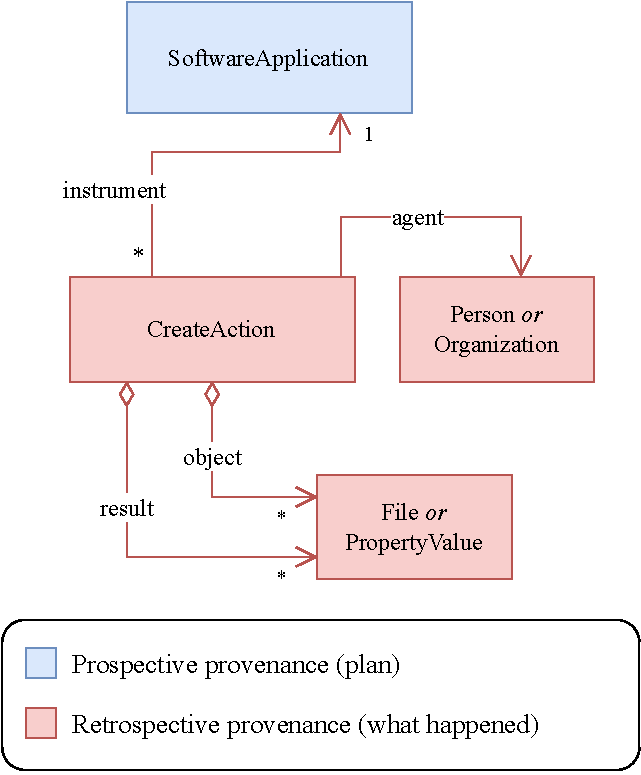
\includegraphics[width=26em]{wrroc-figure1.drawio.pdf}
%DIF >  figure-process-rc-uml
%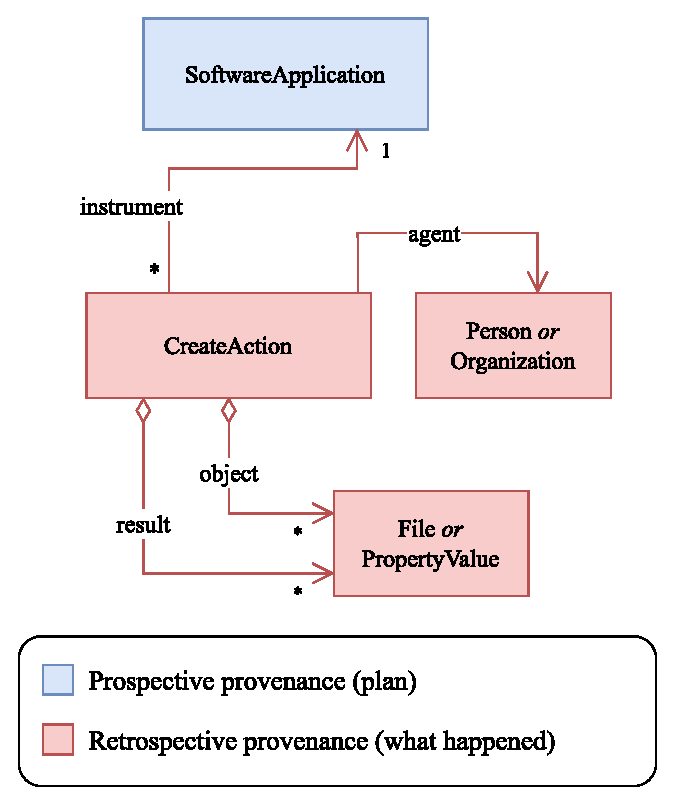
\includegraphics[width=26em]{Fig1.eps}
\caption{{\bf UML class diagram for Process Run Crate.}
The central \DIFdelbeginFL \DIFdelFL{entity }\DIFdelendFL \DIFaddbeginFL \DIFaddFL{class }\DIFaddendFL is the \DIFdelbeginFL \emph{\DIFdelFL{CreateAction}}%DIFAUXCMD
\DIFdelendFL \DIFaddbeginFL \termsorg{CreateAction}\DIFaddendFL , which represents the execution of an application.
It \DIFdelbeginFL \DIFdelFL{relates with }\DIFdelendFL \DIFaddbeginFL \DIFaddFL{links to }\DIFaddendFL the application itself via \DIFdelbeginFL \emph{\DIFdelFL{instrument}}%DIFAUXCMD
\DIFdelendFL \DIFaddbeginFL \termsorg{instrument}\DIFaddendFL , \DIFdelbeginFL \DIFdelFL{with }\DIFdelendFL \DIFaddbeginFL \DIFaddFL{to }\DIFaddendFL the entity that executed it via \DIFdelbeginFL \emph{\DIFdelFL{agent}} %DIFAUXCMD
\DIFdelendFL \DIFaddbeginFL \termsorg{agent}\DIFaddFL{, }\DIFaddendFL and \DIFdelbeginFL \DIFdelFL{with }\DIFdelendFL \DIFaddbeginFL \DIFaddFL{to }\DIFaddendFL its inputs and outputs via \DIFdelbeginFL \emph{\DIFdelFL{object}}
%DIFAUXCMD
\DIFdelendFL \DIFaddbeginFL \termsorg{object}
\DIFaddendFL and \DIFdelbeginFL \emph{\DIFdelFL{result}}%DIFAUXCMD
\DIFdelendFL \DIFaddbeginFL \termsorg{result}\DIFaddendFL , respectively.
\DIFdelbeginFL \emph{\DIFdelFL{File}} %DIFAUXCMD
\DIFdelFL{is an RO-Crate alias for Schema}\DIFdelendFL \DIFaddbeginFL \DIFaddFL{In this and following figures, classes and properties are shown with prefixes to indicate their origin}\DIFaddendFL . \DIFdelbeginFL \DIFdelFL{org's }\emph{\DIFdelFL{MediaObject}}%DIFAUXCMD
\DIFdelFL{.
}\DIFdelendFL %DIF > , note however that the WRROC and RO-Crate JSON-LD contexts map them without needing prefixes. %DG: They do use context, so no prefix is needed...
%DIF > \emph{File} is a mapping in the RO-Crate context to Schema.org's \termsorg{MediaObject}. %SL: we don't mention File anymore
Some inputs (and, less commonly, outputs) \DIFdelbeginFL \DIFdelFL{, however, }\DIFdelendFL are not stored as files or directories, but passed to the application (e.g., via a command line interface) as values of various types (e.g., a number or string). In this case, the profile recommends a representation via \DIFdelbeginFL \emph{\DIFdelFL{PropertyValue}}%DIFAUXCMD
\DIFdelendFL \DIFaddbeginFL \termsorg{PropertyValue}\DIFaddendFL .
For simplicity, we left out the rest of the RO-Crate structure (e.g. the root \DIFdelbeginFL \emph{\DIFdelFL{Dataset}}%DIFAUXCMD
\DIFdelendFL \DIFaddbeginFL \termsorg{Dataset}\DIFaddendFL )\DIFaddbeginFL \DIFaddFL{, and attributes (e.g. }\termsorg{startTime}\DIFaddFL{, }\termsorg{endTime}\DIFaddFL{, }\termsorg{description}\DIFaddFL{, }\termsorg{actionStatus}\DIFaddFL{)}\DIFaddendFL .
In this UML class notation\DIFaddbeginFL \DIFaddFL{, }\DIFaddendFL diamond $\Diamond$ arrows indicate aggregation and regular arrows indicate references, $*$ indicates \DIFdelbeginFL \DIFdelFL{multiple instances}\DIFdelendFL \DIFaddbeginFL \DIFaddFL{zero or more occurrences}\DIFaddendFL , $1$ means single \DIFdelbeginFL \DIFdelFL{instance}\DIFdelendFL \DIFaddbeginFL \DIFaddFL{occurrence}\DIFaddendFL .  
%DIF > Prefix and namespace is \emph{s:} \url{https://schema.org/} %already defined in the table above
}
\label{fig:process_crate_er}
\end{figure}


As an example,
suppose a user \DIFdelbegin \DIFdel{called }\DIFdelend \DIFaddbegin \DIFadd{named }\DIFaddend John Doe runs the \DIFdelbegin \texttt{\DIFdel{head}} %DIFAUXCMD
\DIFdel{UNIX command }\DIFdelend \DIFaddbegin \DIFadd{UNIX command }\texttt{\DIFadd{head}} \DIFaddend to extract the first ten lines of an input file named \texttt{lines.txt}, storing the result in another file called \texttt{selection.txt}.
John then runs the \texttt{sort}
\DIFaddbegin \DIFadd{UNIX }\DIFaddend command on \texttt{selection.txt}, storing the sorted output in a new file named \texttt{sorted\_selection.txt}.
\DIFaddbegin 

\DIFaddend Fig~\ref{fig:head_sort} contains a diagram of the two actions and their relationships to the other \DIFdelbegin \DIFdel{entities involved }\DIFdelend \DIFaddbegin \DIFadd{involved entities}\DIFaddend .
Note how the actions are connected by the fact that the output of ``Run Head'' is also the input of ``Run Sort'': they form an ``implicit workflow'', whose steps have been executed manually rather than by a software tool.

\begin{figure}[!ht]
%DIF < \includegraphics[width=29em]{image2.png}
%DIF < 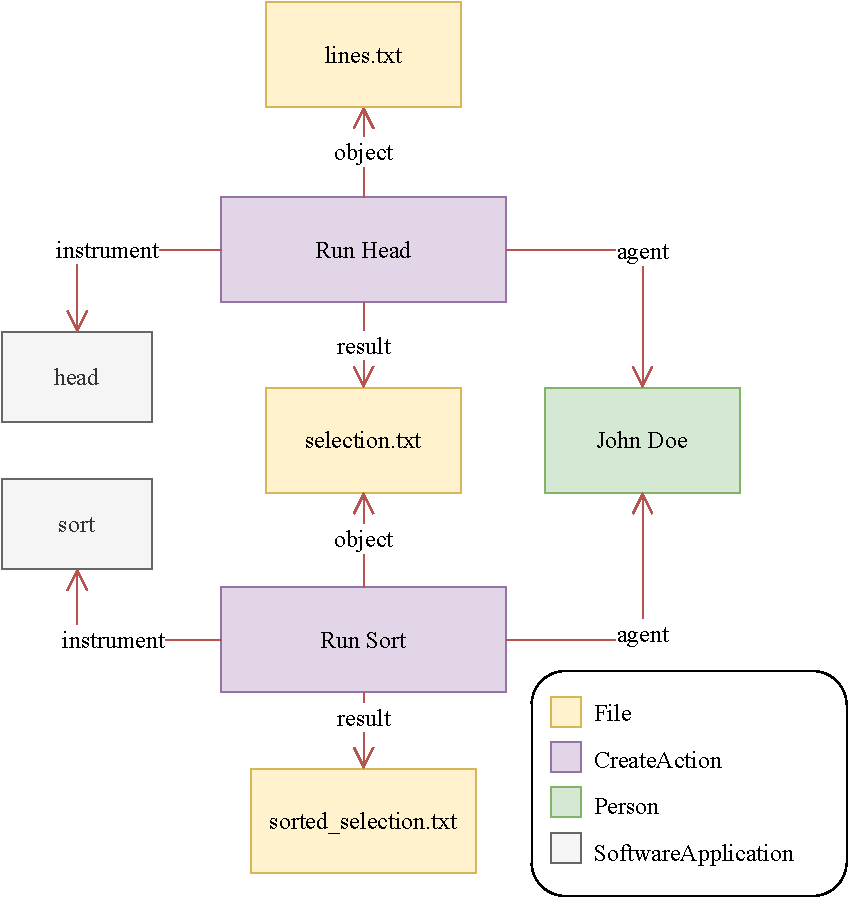
\includegraphics[width=29em]{wrroc-figure-example.drawio.pdf}
%DIF >  figure-example.eps
%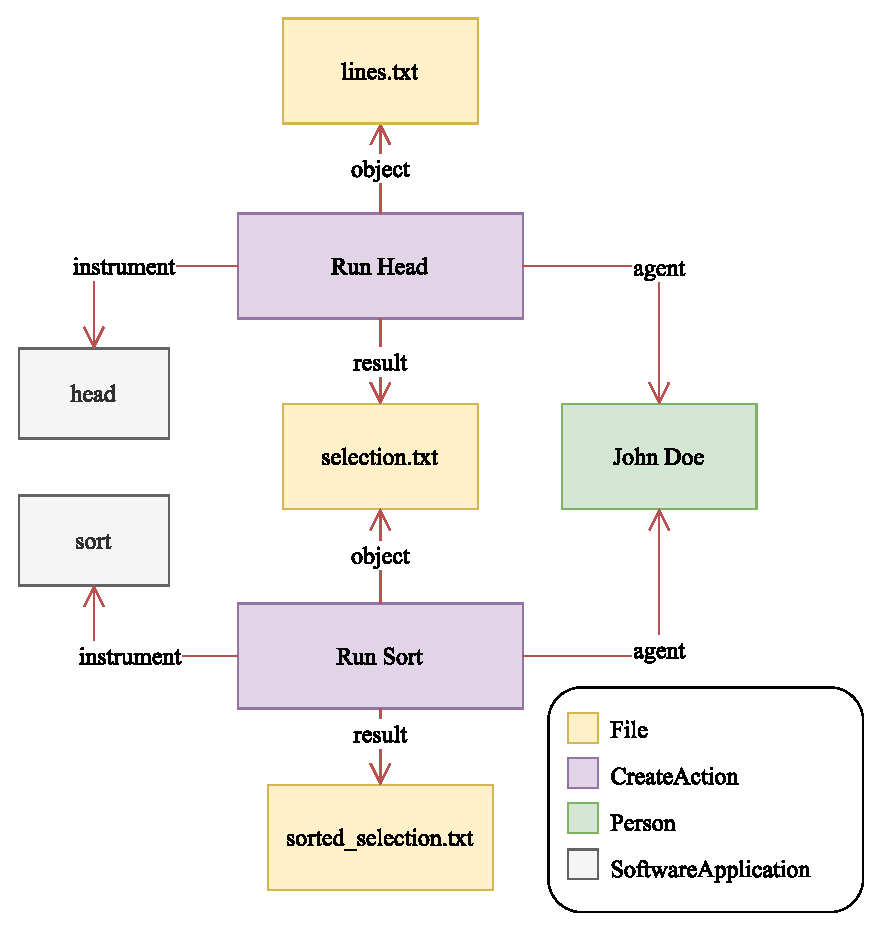
\includegraphics[width=29em]{Fig2.eps}
\caption{{\bf Diagram of a simple workflow} where the \texttt{head} and \texttt{sort} programs were run manually by a user.
The executions of the individual software programs are connected by the fact that the file output by \texttt{head} was used as input for \texttt{sort}, documenting the computational flow in an implicit way.
Such executions can be represented with Process Run Crate.
%DIF > Prefix and namespace: \emph{s:} \url{https://schema.org/}
}
\label{fig:head_sort}
\end{figure}


Process Run Crate extends the RO-Crate guidelines on representing software used to create files with additional requirements and conventions.
This arrangement is typical of the RO-Crate approach, where the base specification provides general recommendations to allow for high flexibility, while profiles -- being more concerned with the representation of specific domains and machine actionability -- provide more detailed and structured definitions.
Nevertheless, in order to be broadly applicable, profiles also need to avoid the specification of too many strict requirements, trying to strike a good trade-off between flexibility and actionability.
\DIFdelbegin \DIFdel{One of the implications of this approach is that consumers need to code defensively, avoiding unwarranted assumptions -- e.g. by verifying that a value exists for an optional property before trying to retrieve it and use it.
}\DIFdelend %DIF > One of the implications of this approach is that consumers need to code defensively, avoiding unwarranted assumptions -- e.g. by verifying that a value exists for an optional property before trying to retrieve it and use it.


\subsection{Workflow Run Crate}\label{workflow-run-crate}

The Workflow Run Crate profile\DIFdelbegin \DIFdel{\mbox{%DIFAUXCMD
\cite{WRROC 2023b} }\hskip0pt%DIFAUXCMD
}\DIFdelend \DIFaddbegin \DIFadd{~\mbox{%DIFAUXCMD
\cite{WRROC 2024b} }\hskip0pt%DIFAUXCMD
}\DIFaddend combines the Process Run Crate and WorkflowHub's Workflow RO-Crate\DIFaddbegin \DIFadd{~}\DIFaddend \cite{Bacall 2022} profiles to describe the execution of \DIFdelbegin \DIFdel{``proper'' }\DIFdelend computational workflows managed by a WMS.
Such workflows are typically written in a \DIFdelbegin \DIFdel{special-purpose }\DIFdelend \DIFaddbegin \DIFadd{domain-specific }\DIFaddend language, such as CWL or Snakemake
\cite{Koster 2012}, and run by one or more WMS (e.g., StreamFlow\DIFaddbegin \DIFadd{~}\DIFaddend \cite{Colonnelli 2021}, Galaxy~\cite{Galaxy 2022}).
\DIFaddbegin \DIFadd{Fig~\ref{fig:workflow_crate_er} illustrates the classes used in this profile together with their relationships.
%DIF > 
}\DIFaddend As in Process Run Crate, the execution is described by a \DIFdelbegin \emph{\DIFdel{CreateAction}}
%DIFAUXCMD
\DIFdelend \DIFaddbegin \termsorg{CreateAction}
\DIFaddend that links to the application via \DIFdelbegin \emph{\DIFdel{instrument}}%DIFAUXCMD
\DIFdelend \DIFaddbegin \termsorg{instrument}\DIFaddend , but in this case the application must be a workflow, as prescribed by Workflow RO-Crate.
More specifically, Workflow RO-Crate states that the RO-Crate must contain a main workflow typed as \emph{File} \DIFdelbegin \DIFdel{, }\emph{\DIFdel{SoftwareSourceCode}}
%DIFAUXCMD
\DIFdel{and }\emph{\DIFdel{ComputationalWorkflow}}%DIFAUXCMD
\DIFdelend \DIFaddbegin \DIFadd{(an RO-Crate mapping to }\termsorg{MediaObject}\DIFadd{), }\termsorg{SoftwareSourceCode}
\DIFadd{and }\termbioschemas{ComputationalWorkflow}\DIFaddend .
The execution of the individual workflow steps, instead, is not represented: that is left to the more detailed Provenance Run Crate profile (described in the next section).

The Workflow Run \DIFdelbegin \DIFdel{RO-Crate }\DIFdelend \DIFaddbegin \DIFadd{Crate }\DIFaddend profile also contains recommendations on how to represent the workflow's input and output parameters, based on the \DIFdelbegin \DIFdel{aforementioned Bioschemas ~\mbox{%DIFAUXCMD
\cite{Gray 2017} }\hskip0pt%DIFAUXCMD
}\DIFdelend \DIFaddbegin \DIFadd{Bioschemas }\DIFaddend ComputationalWorkflow profile.
All these elements are represented via the \DIFdelbegin \emph{\DIFdel{FormalParameter}} %DIFAUXCMD
\DIFdel{entity }\DIFdelend \DIFaddbegin \termbioschemas{FormalParameter} \DIFadd{class }\DIFaddend and are referenced from the main workflow via the \DIFdelbegin \emph{\DIFdel{input}} %DIFAUXCMD
\DIFdel{and
}\emph{\DIFdel{output}} %DIFAUXCMD
\DIFdelend \DIFaddbegin \termbsp{input} \DIFadd{and
}\termbsp{output} \DIFaddend properties.
While the \DIFdelbegin \DIFdel{entities referenced from
}\emph{\DIFdel{object}} %DIFAUXCMD
\DIFdel{and }\emph{\DIFdel{result}} %DIFAUXCMD
\DIFdel{in the }\emph{\DIFdel{CreateAction}} %DIFAUXCMD
\DIFdelend \DIFaddbegin \DIFadd{classes referenced from
}\termsorg{object} \DIFadd{and }\termsorg{result} \DIFadd{in the }\termsorg{CreateAction} \DIFaddend represent data entities and argument values that were actually used in the workflow execution, the ones referenced from \DIFdelbegin \emph{\DIFdel{input}} %DIFAUXCMD
\DIFdel{and
}\emph{\DIFdel{output}} %DIFAUXCMD
\DIFdelend \DIFaddbegin \termbsp{input} \DIFadd{and
}\termbsp{output} \DIFaddend correspond to formal parameters, which acquire a value when the workflow is run (see Fig\DIFdelbegin \DIFdel{.}\DIFdelend ~\ref{fig:workflow_crate_er}).
In the profile, the relationship between an actual value and the corresponding formal parameter is expressed through the \DIFdelbegin \emph{\DIFdel{exampleOfWork}} %DIFAUXCMD
\DIFdel{property-- the downloadable file is a realisation of the formal parameter definition}\DIFdelend \DIFaddbegin \termsorg{exampleOfWork} \DIFadd{property}\DIFaddend .
For instance, in the following JSON-LD snippet a formal parameter (\texttt{\#annotations}) is illustrated together with a corresponding \texttt{final-annotations.tsv} file:
\DIFdelbegin %DIFDELCMD < 

%DIFDELCMD < %%%
\DIFdelend %DIF > 
\begin{verbatim}
{
    "@id": "#annotations",
    "@type": "FormalParameter",
    "additionalType": "File",
    "encodingFormat": "text/tab-separated-values",
    "valueRequired": "True",
    "name": "annotations"
},
{
    "@id": "final-annotations.tsv",
    "@type": "File",
    "contentSize": "14784",
    "exampleOfWork": {"@id": "#annotations"}
}
\end{verbatim}

\DIFdelbegin \DIFdel{The derivation of Workflow Run Crate from Workflow RO-Crate makes RO-Crates that conform to this profile compatible with the WorkflowHub workflow registry by also conforming to its Workflow RO-Crate profile.
Thus, users of a WMS that implements this profile (or Provenance Run Crate, which inherits it) are able to register their workflows in WorkflowHub -- together with an execution trace -- by simply running them and uploading the resulting RO-Crates.
Additionally, the inheritance mechanism allows to reuse the specifications already developed for Workflow RO-Crate, which form part of the guidelines on representing the prospective provenance.
}\DIFdelend %DIF > % This paragraph now moved to  Discussion
%DIF > The derivation of Workflow Run Crate from Workflow RO-Crate makes RO-Crates that conform to this profile compatible with the WorkflowHub workflow registry by also conforming to its Workflow RO-Crate profile.
%DIF > Thus, users of a WMS that implements this profile (or Provenance Run Crate, which inherits it) are able to register their workflows in WorkflowHub -- together with an execution trace -- by simply running them and uploading the resulting RO-Crates.
%DIF > Additionally, the inheritance mechanism allows to reuse the specifications already developed for Workflow RO-Crate, which form part of the guidelines on representing the prospective provenance.

\DIFdelbegin \DIFdel{Fig~\ref{fig:workflow_crate_er} shows the entities used in Workflow Run Crate together with their relationships.
}%DIFDELCMD < 

%DIFDELCMD < \begin{figure}[!h]
%DIFDELCMD < %%%
%DIF < 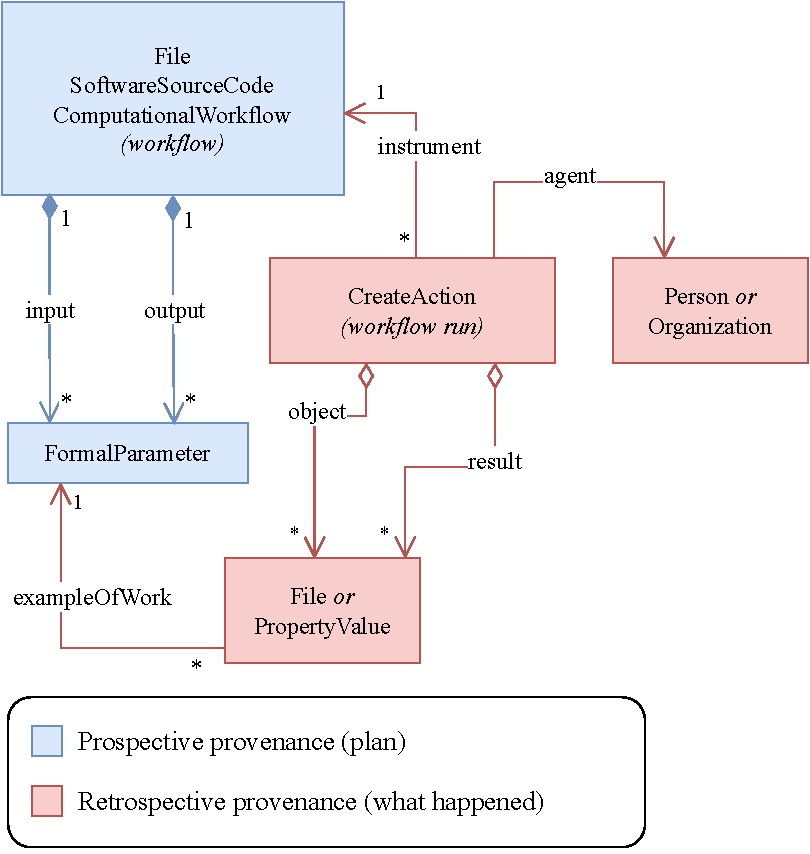
\includegraphics[width=26em]{wrroc-figure2.drawio.pdf}
\DIFdelendFL \DIFaddbeginFL \begin{figure}[!htb]
%DIF >  figure-workflow-rc-uml
\DIFaddendFL %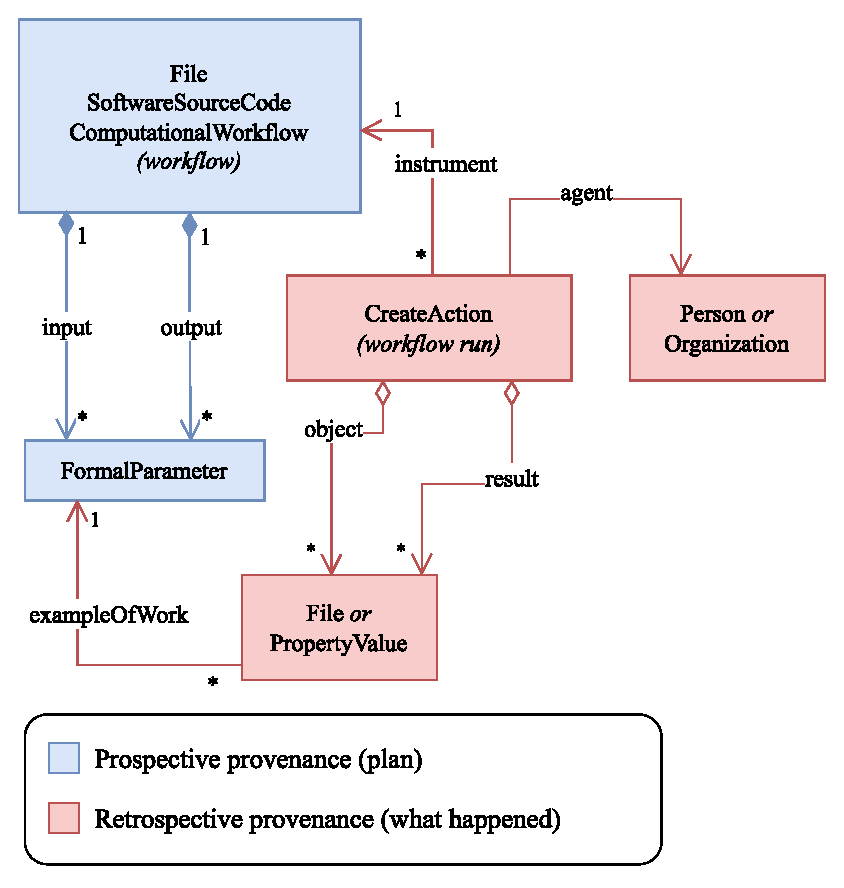
\includegraphics[width=26em]{Fig3.eps}
\caption{{\bf UML class diagram for Workflow Run Crate.}
The main differences with Process Run Crate are the representation of formal parameters and the fact that the \DIFdelbeginFL \DIFdelFL{application }\DIFdelendFL \DIFaddbeginFL \DIFaddFL{workflow }\DIFaddendFL is expected to be an entity with types \DIFaddbeginFL \termsorg{MediaObject} \DIFaddFL{(}\DIFaddendFL \emph{File} \DIFaddbeginFL \DIFaddFL{in RO-Crate JSON-LD)}\DIFaddendFL , \DIFdelbeginFL \emph{\DIFdelFL{SoftwareSourceCode}} %DIFAUXCMD
\DIFdelendFL \DIFaddbeginFL \termsorg{SoftwareSourceCode} \DIFaddendFL and \DIFdelbeginFL \emph{\DIFdelFL{ComputationalWorkflow}}%DIFAUXCMD
\DIFdelendFL \DIFaddbeginFL \termbioschemas{ComputationalWorkflow}\DIFaddendFL .
Effectively, the \DIFdelbeginFL \DIFdelFL{entity }\DIFdelendFL \DIFaddbeginFL \DIFaddFL{workflow }\DIFaddendFL belongs to all three types, and its properties are the union of the properties of the individual types.
\DIFaddbeginFL \DIFaddFL{In this profile, the execution history (retrospective provenance) is augmented by a (prospective) workflow definition, giving a high-level overview of the workflow and its input and output parameter definitions (}\termbioschemas{FormalParameter}\DIFaddFL{). }\DIFaddendFL The \DIFaddbeginFL \DIFaddFL{inner structure of the workflow is not represented in this profile.
In the provenance part, individual files (}\termsorg{MediaObject}\DIFaddFL{) or arguments (}\termsorg{PropertyValue}\DIFaddFL{) are then connected to the parameters they realise. Most workflow systems can consume and produce multiple files, and this mechanism helps to declare each file's role in the workflow execution.
The }\DIFaddendFL filled diamond $\blacklozenge$ indicates composition, empty diamond $\Diamond$ aggregation, and other arrows relations.
%DIF > Prefixes and namespaces are 
%DIF > \emph{s:} \url{https://schema.org/}\hspace{1ex}
%DIF > \emph{bioschemas:} \url{https://bioschemas.org/}\hspace{1ex}
%DIF > \emph{bsp:} \url{https://bioschemas.org/properties/}
%DIF > DG: altrady added in the table before figs, I think it's not needed to add them again
}
\label{fig:workflow_crate_er}
\end{figure}


\subsection{Provenance Run Crate}\label{provenance-run-crate}

The Provenance Run Crate profile\DIFdelbegin \DIFdel{\mbox{%DIFAUXCMD
\cite{WRROC 2023c} }\hskip0pt%DIFAUXCMD
}\DIFdelend \DIFaddbegin \DIFadd{~\mbox{%DIFAUXCMD
\cite{WRROC 2024c} }\hskip0pt%DIFAUXCMD
}\DIFaddend extends Workflow Run Crate by adding new concepts to describe the internal details of a workflow run, including individual tool executions, intermediate outputs and related parameters.
Individual tool executions are represented by additional \DIFdelbegin \emph{\DIFdel{CreateAction}} %DIFAUXCMD
\DIFdelend \DIFaddbegin \termsorg{CreateAction} \DIFaddend instances that refer to the tool itself via \DIFdelbegin \emph{\DIFdel{instrument}} %DIFAUXCMD
\DIFdelend \DIFaddbegin \termsorg{instrument} \DIFaddend -- analogously to its use in Process Run Crate.
The workflow is required to refer to the tools it orchestrates through the \DIFdelbegin \emph{\DIFdel{hasPart}} %DIFAUXCMD
\DIFdelend \DIFaddbegin \termsorg{hasPart} \DIFaddend property, as suggested in the Bioschemas ComputationalWorkflow profile, though in the latter it is only a recommendation.

To represent the logical steps defined by the workflow, this profile uses \DIFdelbegin \emph{\DIFdel{HowToStep}} %DIFAUXCMD
\DIFdel{i.e., ``}\DIFdelend \DIFaddbegin \termsorg{HowToStep} \DIFadd{-- i.e., “}\DIFaddend A step in the instructions for how to achieve a result\DIFdelbegin \DIFdel{'' (}%DIFDELCMD < \url{https://schema.org/HowToStep}%%%
\DIFdel{)}\DIFdelend \DIFaddbegin \DIFadd{”~\mbox{%DIFAUXCMD
\cite{howtostep-def}}\hskip0pt%DIFAUXCMD
}\DIFaddend .
Steps point to the corresponding tools via the \DIFdelbegin \emph{\DIFdel{workExample}} %DIFAUXCMD
\DIFdelend \DIFaddbegin \termsorg{workExample} \DIFaddend property and are referenced from the workflow via the \DIFdelbegin \emph{\DIFdel{step}} %DIFAUXCMD
\DIFdelend \DIFaddbegin \termsorg{step} \DIFaddend property; the execution of a step is represented by a \DIFdelbegin \emph{\DIFdel{ControlAction}} %DIFAUXCMD
\DIFdelend \DIFaddbegin \termsorg{ControlAction} \DIFaddend pointing to the
\DIFdelbegin \emph{\DIFdel{HowToStep}} %DIFAUXCMD
\DIFdel{via }\emph{\DIFdel{instrument}} %DIFAUXCMD
\DIFdelend \DIFaddbegin \termsorg{HowToStep} \DIFadd{via }\termsorg{instrument} \DIFaddend and to the \DIFdelbegin \emph{\DIFdel{CreateAction}}
%DIFAUXCMD
\DIFdel{instance(s) }\DIFdelend \DIFaddbegin \termsorg{CreateAction}
\DIFadd{entities }\DIFaddend that represent the corresponding tool execution(s) via
\DIFdelbegin \emph{\DIFdel{object}}%DIFAUXCMD
\DIFdelend \DIFaddbegin \termsorg{object}\DIFaddend .
Note that a step execution does not coincide with a tool execution: an example where this distinction is apparent is when a step maps to multiple executions of the same tool over a list of inputs (e.g. the ``scattering'' feature in CWL).

An RO-Crate following this profile can also represent the execution of the WMS itself (e.g., cwltool) via
\DIFdelbegin \emph{\DIFdel{OrganizeAction}}%DIFAUXCMD
\DIFdelend \DIFaddbegin \termsorg{OrganizeAction}\DIFaddend , pointing to a representation of the WMS via
\DIFdelbegin \emph{\DIFdel{instrument}}%DIFAUXCMD
\DIFdelend \DIFaddbegin \termsorg{instrument}\DIFaddend , to the steps via \DIFdelbegin \emph{\DIFdel{object}} %DIFAUXCMD
\DIFdelend \DIFaddbegin \termsorg{object} \DIFaddend and to the workflow run via \DIFdelbegin \emph{\DIFdel{result}}%DIFAUXCMD
\DIFdel{.
The }\emph{\DIFdel{object}} %DIFAUXCMD
\DIFdelend \DIFaddbegin \termsorg{result}\DIFadd{.
The }\termsorg{object} \DIFaddend attribute of the
\DIFdelbegin \emph{\DIFdel{OrganizeAction}} %DIFAUXCMD
\DIFdelend \DIFaddbegin \termsorg{OrganizeAction} \DIFaddend can additionally point to a configuration file containing a description of the settings that affected the behaviour of the WMS during the execution.
\DIFdelbegin %DIFDELCMD < 

%DIFDELCMD < %%%
\DIFdelend %DIF > 
Fig~\ref{fig:provenance_crate_er} \DIFdelbegin \DIFdel{shows the various entities }\DIFdelend \DIFaddbegin \DIFadd{illustrates the various classes }\DIFaddend involved in the representation of a workflow run via Provenance Run Crate together with their relationships.

\DIFdelbegin %DIFDELCMD < \begin{figure}[!h]
%DIFDELCMD < %%%
%DIF < \includegraphics[width=21em]{image4.png}
%DIF < 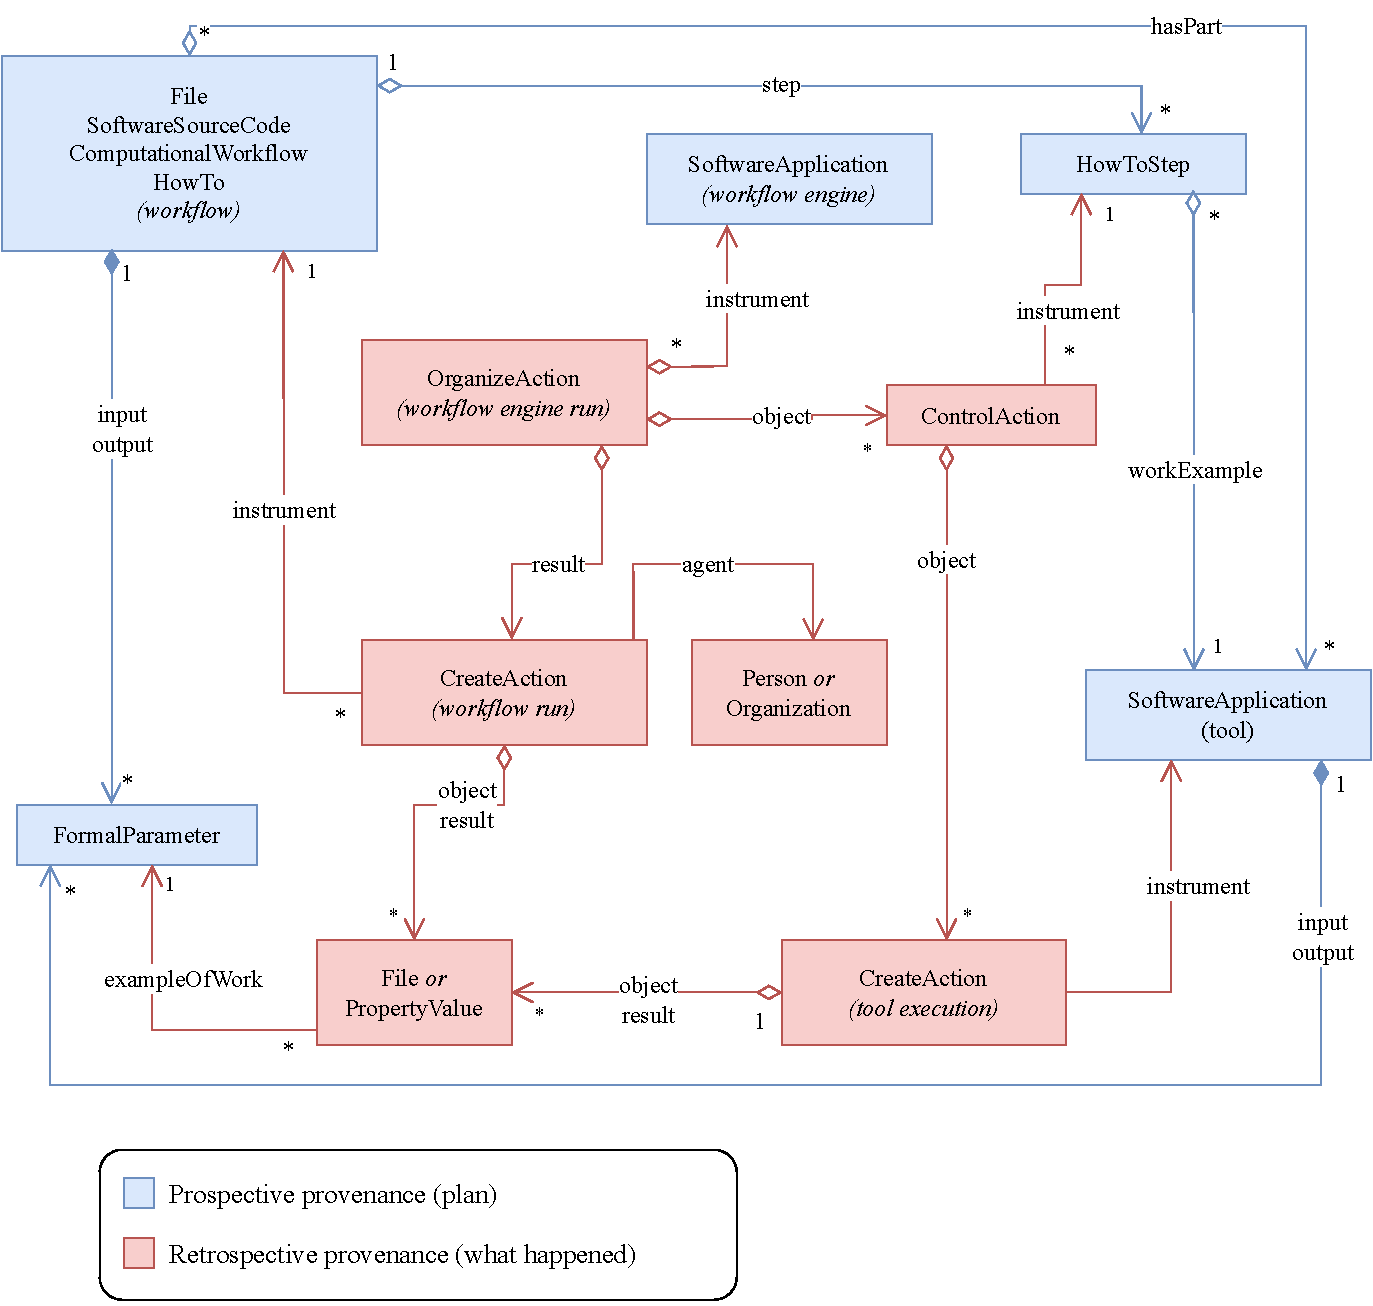
\includegraphics[width=\textwidth]{wrroc-figure3.drawio.pdf}
\DIFdelendFL \DIFaddbeginFL \begin{figure}[!htb]
%DIF > figure-provenance-rc-uml
\DIFaddendFL %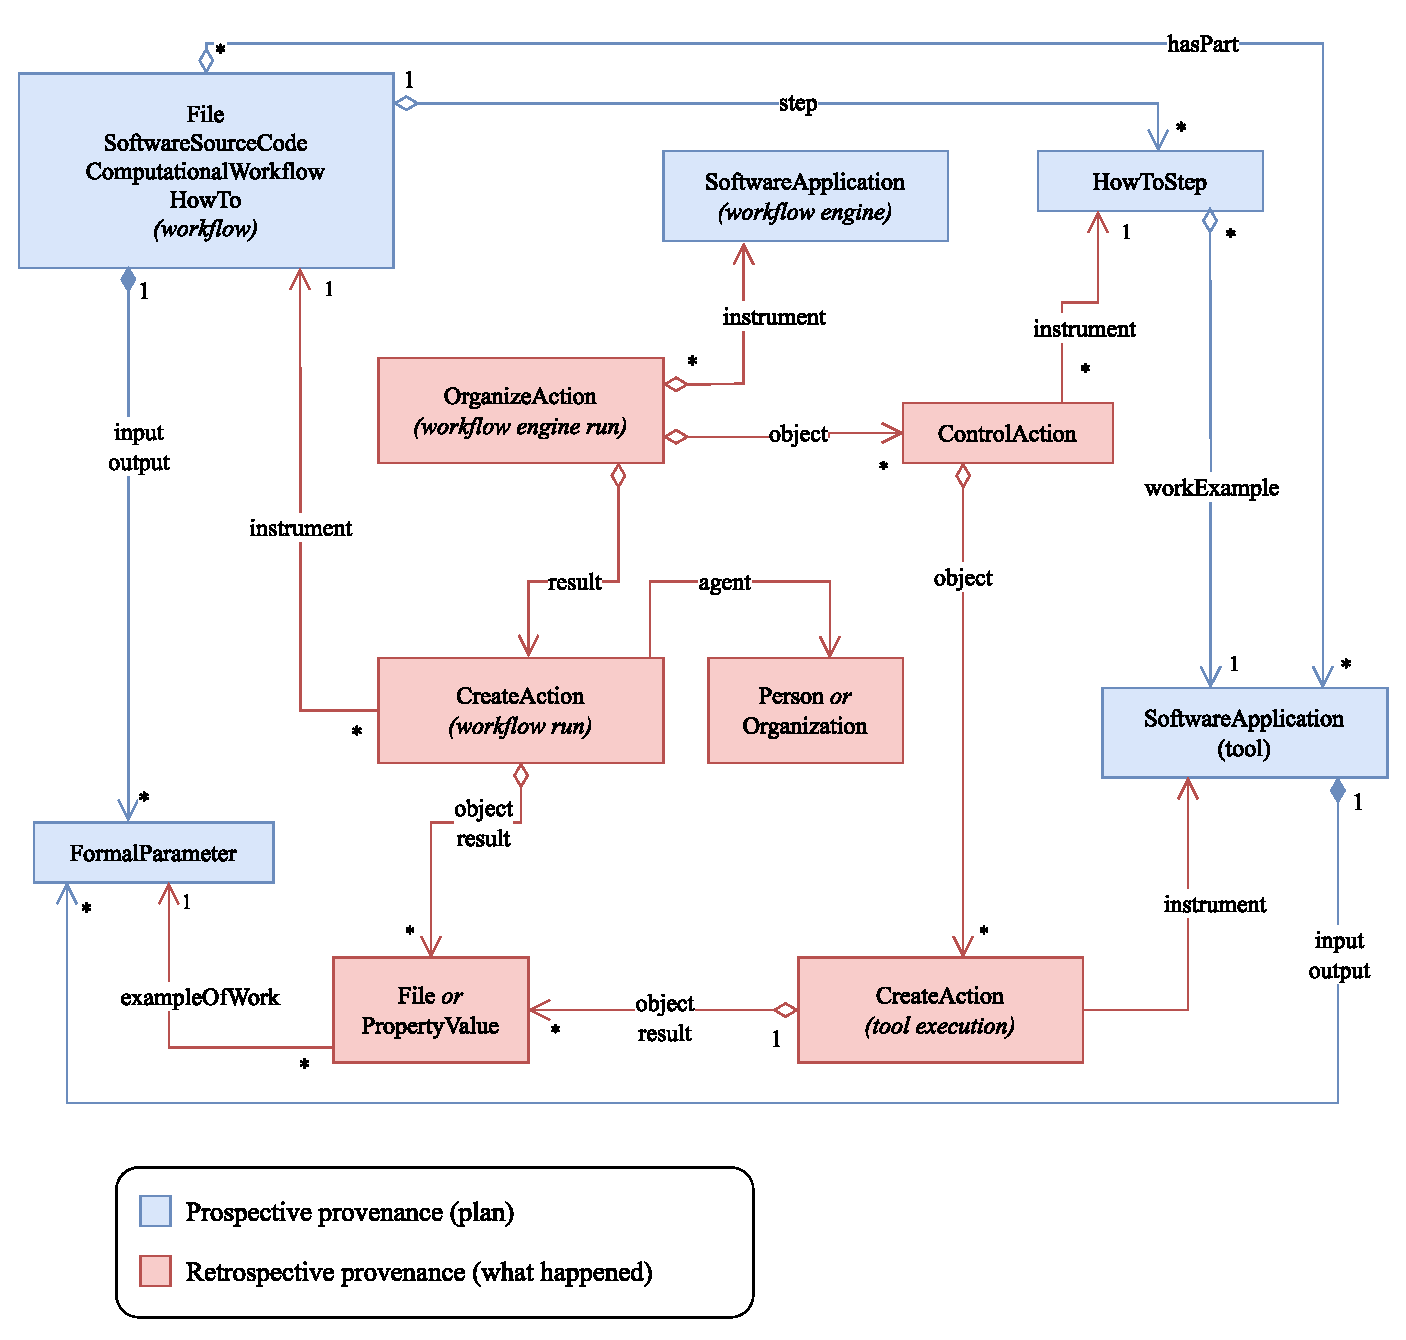
\includegraphics[width=\textwidth]{Fig4.eps}
\caption{{\bf UML class diagram for Provenance Run Crate.}
In addition to the workflow run, this profile represents the execution of individual steps and their related tools.
\DIFaddbeginFL \DIFaddFL{The prospective side (the execution plan) is shown by the workflow listing a series of }\termsorg{HowToStep}\DIFaddFL{s, each linking to the }\termsorg{SoftwareApplication} \DIFaddFL{that is to be executed. The }\termbsp{input} \DIFaddFL{and }\termbsp{output} \DIFaddFL{parameters for each tool are described in a similar way to the overall workflow parameter in Fig~\ref{fig:workflow_crate_er}.
The retrospective provenance side of this profile includes each tool execution as an additional }\termsorg{CreateAction} \DIFaddFL{with similar mapping to the realised parameters as }\termsorg{MediaObject} \DIFaddFL{or }\termsorg{PropertyValue}\DIFaddFL{, allowing intermediate values to be included in the RO-Crate even if they are not workflow outputs.
The workflow execution is described the same as in the Workflow Run Crate profile with an overall }\termsorg{CreateAction} \DIFaddFL{(the workflow outputs will typically also appear as outputs from inner tool executions). An additional }\termsorg{OrganizeAction} \DIFaddFL{represents the workflow engine execution, which orchestrated the steps from the workflow plan through corresponding }\termsorg{ControlAction}\DIFaddFL{s that spawned the tool's execution (}\termsorg{CreateAction}\DIFaddFL{). It is possible that a single workflow step had multiple such executions (e.g. array iterations). Not shown in figure: }\termsorg{actionStatus} \DIFaddFL{and }\termsorg{error} \DIFaddFL{to indicate step/workflow execution status.
The filled diamond $\blacklozenge$ indicates composition, empty diamond $\Diamond$ aggregation, and other arrows relations.
%DIF > Prefixes and namespaces are 
%DIF > \emph{s:} \url{https://schema.org/}\hspace{1ex}
%DIF > \emph{bioschemas:} \url{https://bioschemas.org/}\hspace{1ex}
%DIF > \emph{bsp:} \url{https://bioschemas.org/properties/}
}\DIFaddendFL }
\label{fig:provenance_crate_er}
\end{figure}

\DIFdelbegin \DIFdel{This profile also includes specifications on }\DIFdelend \DIFaddbegin \DIFadd{Additionally, this profile specifies }\DIFaddend how to describe connections between parameters\DIFdelbegin \DIFdel{.
Parameter connections }\DIFdelend \DIFaddbegin \DIFadd{,
through }\textit{\DIFadd{parameter connections}} \DIFaddend -- a fundamental feature of computational workflows\DIFdelbegin \DIFdel{-- describe}\DIFdelend \DIFaddbegin \DIFadd{.
Specifically, parameter connections describe: }\DIFaddend (i) how tools \DIFdelbegin \DIFdel{take }\DIFdelend \DIFaddbegin \DIFadd{consume }\DIFaddend as input the intermediate outputs generated by other tools\DIFaddbegin \DIFadd{; }\DIFaddend and (ii) how workflow-level parameters are mapped to tool-level parameters.
\DIFdelbegin \DIFdel{For instance}\DIFdelend \DIFaddbegin \DIFadd{As an example}\DIFaddend , consider again the workflow depicted in Fig\DIFdelbegin \DIFdel{. }\DIFdelend ~\ref{fig:head_sort},
and suppose it is implemented in a workflow language such as CWL\DIFdelbegin \DIFdel{. The }\DIFdelend \DIFaddbegin \DIFadd{: the }\DIFaddend workflow-level input (a text file) is \DIFdelbegin \DIFdel{connected }\DIFdelend \DIFaddbegin \DIFadd{linked through a parameter connection }\DIFaddend to the input of the \DIFdelbegin \DIFdel{``head'' }\DIFdelend \DIFaddbegin \texttt{\DIFadd{head}} \DIFaddend tool wrapper, and \DIFdelbegin \DIFdel{the output of the latter is connected }\DIFdelend \DIFaddbegin \DIFadd{then a second parameter connection links this tool's output }\DIFaddend to the input of the \DIFdelbegin \DIFdel{``sort'' }\DIFdelend \DIFaddbegin \texttt{\DIFadd{sort}} \DIFaddend tool wrapper.
\DIFdelbegin %DIFDELCMD < 

%DIFDELCMD < %%%
\DIFdelend %DIF > 
A representation of parameter connections is particularly useful for traceability, since it \DIFdelbegin \DIFdel{allows }\DIFdelend \DIFaddbegin \DIFadd{provides the means }\DIFaddend to document the inputs and tools on which workflow outputs depend.
Since the current RO-Crate context has no suitable terms for the description of such relationships,
we added appropriate ones to the aforementioned \DIFdelbegin \DIFdel{``workflow-run'' context extension (the }%DIFDELCMD < \url{https://w3id.org/ro/terms/workflow-run\#} %%%
\DIFdel{namespace):
a }\emph{\DIFdel{ParameterConnection}} %DIFAUXCMD
\DIFdel{type with
}\emph{\DIFdel{sourceParameter}} %DIFAUXCMD
\DIFdel{and }\emph{\DIFdel{targetParameter}} %DIFAUXCMD
\DIFdelend \DIFaddbegin \DIFadd{dedicated term set~\mbox{%DIFAUXCMD
\cite{wrroc-terms}}\hskip0pt%DIFAUXCMD
:
a }\termwfrun{ParameterConnection} \DIFadd{type with
}\termwfrun{sourceParameter} \DIFadd{and }\termwfrun{targetParameter} \DIFaddend attributes that respectively map to the source and target formal parameters, and a
\DIFdelbegin \emph{\DIFdel{connection}} %DIFAUXCMD
\DIFdelend \DIFaddbegin \termwfrun{connection} \DIFaddend property to link from the relevant step or workflow to the \DIFdelbegin \emph{\DIFdel{ParameterConnection}} %DIFAUXCMD
\DIFdelend \DIFaddbegin \termwfrun{ParameterConnection} \DIFaddend instances.

\DIFdelbegin \DIFdel{This profile }\DIFdelend \DIFaddbegin \DIFadd{In our set of profiles, Provenance Run Crate }\DIFaddend is the most detailed \DIFdelbegin \DIFdel{of the three, }\DIFdelend \DIFaddbegin \DIFadd{one }\DIFaddend and offers the highest level of granularity\DIFdelbegin \DIFdel{. Fig.~\ref{fig:profile_venn}shows the relationship between the specifications of the profiles as a Venn diagram. }\DIFdelend \DIFaddbegin \DIFadd{; its specification is a superset of Workflow Run RO-Crate, which in turn is a superset of Process Run Crate. This relationship between the three profiles is illustrated in Fig~\ref{fig:profile_venn}, as a Venn diagram.
Theoretically, all computational provenance information could be represented through the Provenance Run Crate profile alone (possibly relaxing some requirements), since it inherits from the other ones. In practice, though, this choice would require the use of the most complex model even for simple use cases. Having three separate profiles provides a way to represent information at different levels of granularity, while keeping all RO-Crates generated with them interoperable. This approach gives a straightforward path to supporting the representation of computational provenance in simpler use cases such as with simple command executions, i.e. the Process Run Crate. Additionally, the approach lowers the accessibility barrier for implementation in WMSs, as developers may choose to initially implement only the more basic support in their WMS, with reduced effort and complexity, and gradually scale to more detailed representations. This encourages the adoption of WRROC across the diverse landscape of use cases and WMSs.
}\DIFaddend 

\DIFdelbegin %DIFDELCMD < \begin{figure}[!h]
%DIFDELCMD < %%%
%DIF <   \includegraphics[width=21em]{venn.png}
  %DIF < 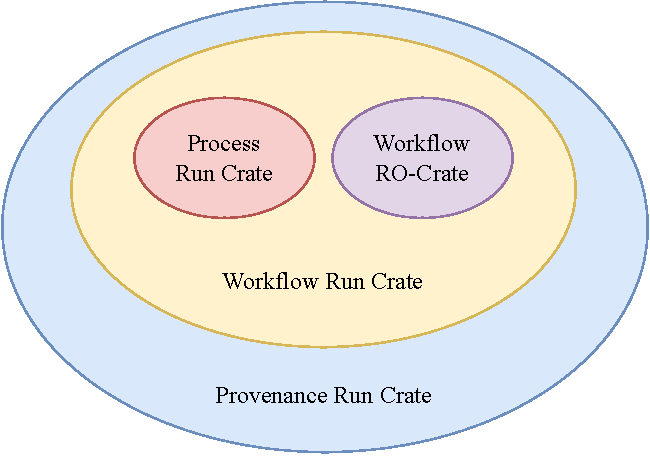
\includegraphics[width=26em]{wrroc-venn.drawio.pdf}
  \DIFdelendFL \DIFaddbeginFL \begin{figure}[htb]
  %DIF >  figure-venn.eps
  \DIFaddendFL %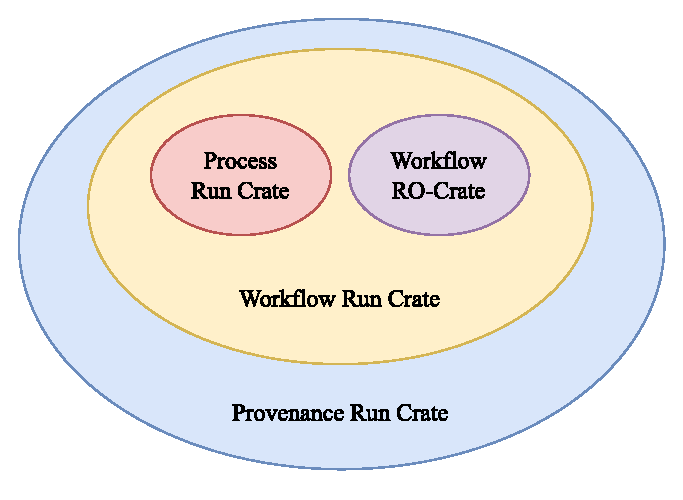
\includegraphics[width=26em]{Fig5.eps}
  \caption{{\bf Venn diagram of the specifications for the various RO-Crate profiles.}
  \DIFaddbeginFL \DIFaddFL{Process Run Crate specifies how to describe the fundamental classes involved in a computational run, and thus is the basis for all profiles in the WRROC collection.
  }\DIFaddendFL Workflow Run Crate inherits the specifications of both Process Run Crate and Workflow RO-Crate. Provenance Run Crate, in turn, inherits the specifications of Workflow Run Crate \DIFaddbeginFL \DIFaddFL{(and in a sense includes multiple Process Runs for each step execution, but within a single Crate)}\DIFaddendFL .
  }
  \label{fig:profile_venn}
  \end{figure}


\DIFaddbegin \subsection{\DIFadd{Profile formats}}\label{profile-formats}

\DIFadd{The WRROC profiles are available both in human-readable (HTML) and in machine-readable format (RO-Crate). The human-readable profiles are at:
%DIF > 
}\begin{itemize}
    \item \url{https://w3id.org/ro/wfrun/process/0.5}
    \item \url{https://w3id.org/ro/wfrun/workflow/0.5}
    \item \url{https://w3id.org/ro/wfrun/provenance/0.5}
\end{itemize}
%DIF > 
\DIFadd{And the corresponding machine-readable ones at:
%DIF > 
}\begin{itemize}
    \item \url{https://doi.org/10.5281/zenodo.12158562}
    \item \url{https://doi.org/10.5281/zenodo.12159311}
    \item \url{https://doi.org/10.5281/zenodo.12160782}
\end{itemize}
%DIF > 
\DIFadd{The RO-Crate metadata files for the machine readable profiles can be retrieved using the same URLs as the human-readable ones, but with JSON-LD content negotiation: this is done by setting }\texttt{\DIFadd{"Accept:application/ld+json"}} \DIFadd{in the HTTP header.
}

\DIFadd{The new terms we defined to represent concepts that could not be expressed with existing Schema.org ones are at:
%DIF > 
}\begin{itemize}
    \item \url{https://w3id.org/ro/terms/workflow-run}
\end{itemize}
%DIF > 
\DIFadd{These terms are available in multiple formats with content negotiation, as explained at the above link.
}

\DIFaddend %%
\section{Implementations}\label{implementations}

Support for the Workflow Run RO-Crate profiles presented in this work has been implemented in a number of systems, showing support from the community and demonstrating their usability in practice.
We describe seven of these implementations (one in a conversion tool and six in WMS) in the following sections.
\DIFaddbegin \DIFadd{Table~\ref{implementation_summary_table} provides an overview of the implementations, along with the respective profile implemented, and links to the implementation itself and to an example RO-Crate.
%DIF > 
}\DIFaddend These tools have been developed in parallel by different teams, and independently from each other.
RO-Crate has a strong ecosystem of tools\DIFaddbegin \DIFadd{~}\DIFaddend \cite{Soiland-Reyes 2022a}, and \DIFdelbegin \DIFdel{these }\DIFdelend \DIFaddbegin \DIFadd{the WRROC }\DIFaddend implementations have either re-used these or added their own approach to the standards.


\subsection{Runcrate}\label{runcrate}

Runcrate\DIFdelbegin \DIFdel{(}%DIFDELCMD < \url{https://github.com/ResearchObject/runcrate}%%%
\DIFdel{) }\DIFdelend \DIFaddbegin \DIFadd{~}\DIFaddend \cite{runcrate} is a Workflow Run RO-Crate toolkit which also serves as a reference implementation of the proposed profiles.
It consists of a Python package with a command line interface, providing a straightforward path to integration in Python software and other workflows.
The runcrate toolkit includes functionality to convert CWLProv ROs to RO-Crates conforming to the Provenance Run Crate profile (\DIFdelbegin \emph{\DIFdel{runcrate convert}}%DIFAUXCMD
\DIFdelend \DIFaddbegin \texttt{\DIFadd{runcrate convert}}\DIFaddend ), effectively providing an indirect implementation of the format for cwltool.
Indeed, the CWLProv model provided a basis for the Provenance Run Crate profile, and the implementation of a conversion tool in runcrate at times drove the improvement and extension of the profile as new requirements or gaps in the old designs emerged.
Runcrate converts both the retrospective provenance part of the CWLProv RO (the RDF graph of the workflow's execution) and the prospective provenance part (the CWL files, including the workflow itself).
Both parts are thus converted into a single, \DIFdelbegin \DIFdel{workflow language-agnostic }\DIFdelend \DIFaddbegin \DIFadd{workflow-language-agnostic }\DIFaddend metadata resource.

Another functionality offered by the runcrate package is \DIFdelbegin \emph{\DIFdel{runcrate report}} %DIFAUXCMD
\DIFdelend \DIFaddbegin \texttt{\DIFadd{runcrate report}}\DIFadd{, }\DIFaddend which reports on the various executions described in an input RO-Crate, listing their starting and ending times, the values of the various parameters, etc.
Runcrate report demonstrates how the provenance profiles presented in this work enable comparison of runs interoperably across different workflow languages or different implementations of the same language.
This functionality has also been used as a lightweight validator for the various implementations.

\DIFdelbegin \DIFdel{We also added a }\emph{\DIFdel{run}} %DIFAUXCMD
\DIFdelend \DIFaddbegin \DIFadd{Runcrate also includes a }\texttt{\DIFadd{run}} \DIFaddend subcommand to re-execute the computation described by an input Workflow Run Crate or Provenance Run Crate where CWL \DIFdelbegin \DIFdel{was }\DIFdelend \DIFaddbegin \DIFadd{is }\DIFaddend used as a workflow language.
It works by mapping the RO-Crate description of input parameters and their values (the workflow's
\DIFdelbegin \emph{\DIFdel{input}} %DIFAUXCMD
\DIFdelend \DIFaddbegin \termbsp{input} \DIFaddend and the action's \DIFdelbegin \emph{\DIFdel{object}}%DIFAUXCMD
\DIFdelend \DIFaddbegin \termsorg{object}\DIFaddend ) to the format expected by CWL, which is then used to relaunch the workflow on the input data.
This functionality shows the machine-actionability of the profiles to support reproducibility, and was used to successfully re-execute the digital pathology annotation workflow described in \DIFdelbegin \DIFdel{section \ref{provenance-run-crate-for-digital-pathology}.
}%DIFDELCMD < 

%DIFDELCMD < %%%
\DIFdelend \DIFaddbegin \DIFadd{Section~\ref{provenance-run-crate-for-digital-pathology}.
%DIF > 
}\DIFaddend Of course, achieving a full re-execution in the general case may not always be possible: reproducibility is supported by the profiles, but also benefits from \DIFdelbegin \DIFdel{the }\DIFdelend \DIFaddbegin \DIFadd{specific }\DIFaddend characteristics of the workflow language (which should provide a clear formalism to map input items to their corresponding parameter slots) and \DIFdelbegin \DIFdel{from cooperation on the part of the }\DIFdelend \DIFaddbegin \DIFadd{of the specific }\DIFaddend workflow's \DIFdelbegin \DIFdel{author, who can help considerably by containerizing the }\DIFdelend \DIFaddbegin \DIFadd{implementation, which can be made considerably easier to reproduce by containerising the computational }\DIFaddend environment required by each step \DIFdelbegin \DIFdel{and providing the relevant annotations }\DIFdelend (if allowed by the workflow language).


\subsection{Galaxy}\label{galaxy}

The Galaxy project~\cite{Galaxy 2022} provides a WMS with data management functionalities as a multi-user platform, aiming to make computational biology more accessible to research scientists that do not have computer programming or systems administration experience.
Galaxy's most prominent features include: a collection of 7500+ integrated tools\DIFdelbegin \DIFdel{(}%DIFDELCMD < \url{https://galaxyproject.org/toolshed/}%%%
\DIFdel{)}\DIFdelend \DIFaddbegin \DIFadd{~\mbox{%DIFAUXCMD
\cite{Blankenberg 2014}}\hskip0pt%DIFAUXCMD
}\DIFaddend ;
a web interface that allows the \DIFdelbegin \DIFdel{execution and definition }\DIFdelend \DIFaddbegin \DIFadd{definition and execution }\DIFaddend of workflows using the integrated tools; a network of dedicated (public) Galaxy instances.

The export of workflow execution provenance data as Workflow Run Crates \DIFdelbegin \DIFdel{has been added in Galaxy 's 23.0 release.
This feature provides }\DIFdelend \DIFaddbegin \DIFadd{was added to Galaxy in version 23~\mbox{%DIFAUXCMD
\cite{Galaxy 2023} }\hskip0pt%DIFAUXCMD
providing }\DIFaddend a more interoperable alternative to the basic export of Galaxy workflow
\emph{invocations}\DIFaddbegin \DIFadd{. A WRROC export from Galaxy includes}\DIFaddend : the workflow definition; a set of serialisations of the invocation-related metadata in Galaxy native, \DIFdelbegin \DIFdel{json-formatted }\DIFdelend \DIFaddbegin \DIFadd{JSON-formatted }\DIFaddend files;
and the input and output data files.
This \DIFaddbegin \DIFadd{result }\DIFaddend is achieved by\DIFdelbegin \DIFdel{extracting provenance }\DIFdelend \DIFaddbegin \DIFadd{:
}\begin{inlineenum}
\item \DIFadd{extracting provenance data }\DIFaddend from Galaxy entities related to the workflow run, along with \DIFdelbegin \DIFdel{associated metadata, }\DIFdelend \DIFaddbegin \DIFadd{their associated metadata;
}\item \DIFaddend converting them to RO-Crate metadata using the ro-crate-py library~\cite{ro-crate-py};
\DIFdelbegin \DIFdel{by }\DIFdelend \DIFaddbegin \item \DIFaddend describing all files contained in the basic invocation export within the \DIFdelbegin \DIFdel{RO-crate }\DIFdelend \DIFaddbegin \DIFadd{RO-Crate }\DIFaddend metadata; and
\DIFdelbegin \DIFdel{finally by }\DIFdelend \DIFaddbegin \item \DIFaddend making the Workflow Run Crate available for export to the user through Galaxy's web interface and API\DIFaddbegin \DIFadd{~}\DIFaddend \cite{De Geest 2022b}.
\DIFdelbegin %DIFDELCMD < 

%DIFDELCMD < %%%
\DIFdelend \DIFaddbegin \end{inlineenum}
\DIFaddend We extract the prospective provenance contained in Galaxy's YAML-based gxformat2
\DIFdelbegin \DIFdel{(}%DIFDELCMD < \url{https://galaxyproject.github.io/gxformat2/v19_09.html}%%%
\DIFdel{) }\DIFdelend \DIFaddbegin \DIFadd{\mbox{%DIFAUXCMD
\cite{gxformat2} }\hskip0pt%DIFAUXCMD
}\DIFaddend workflow definition, which includes details of the analysis pipeline such as the graph of \DIFaddbegin \DIFadd{the }\DIFaddend tools that need to be executed \DIFdelbegin \DIFdel{, }\DIFdelend and metadata about the data types required.
The retrospective provenance -- i.e., the details of the executed workflow\DIFaddbegin \DIFadd{, }\DIFaddend such as the inputs, outputs, \DIFaddbegin \DIFadd{and }\DIFaddend parameter values used -- is extracted from Galaxy's data model\DIFdelbegin \DIFdel{(}%DIFDELCMD < \url{https://docs.galaxyproject.org/en/master/lib/galaxy.model.html}%%%
\DIFdel{),
}\DIFdelend \DIFaddbegin \DIFadd{,
%DIF > (\url{https://docs.galaxyproject.org/en/master/lib/galaxy.model.html})
}\DIFaddend which is not directly accessible to users in the context of a public Galaxy server.
All of this provenance information is then mapped to RO-Crate metadata, including some Galaxy-specific data entities such as dataset collections.
An exemplary \DIFdelbegin \DIFdel{exported Galaxy }\DIFdelend Workflow Run Crate \DIFaddbegin \DIFadd{exported from Galaxy, through its }\emph{\DIFadd{Workflow Invocations}} \DIFadd{list, }\DIFaddend is available on Zenodo~\cite{De Geest 2023}.

%DIF >  The following procedure description is useful in case reviewers want to try obtaining a WRROC from a Galaxy instance.
In practice, a user would take the following steps to obtain a Workflow Run Crate from a Galaxy instance:
\DIFdelbegin \DIFdel{(1) }\DIFdelend \DIFaddbegin \begin{inlineenum}
\item \DIFaddend create or download a Galaxy workflow definition (e.g.: from WorkflowHub) and import it in a Galaxy instance, or create a workflow through the Galaxy GUI directly;
\DIFdelbegin \DIFdel{(2) }\DIFdelend \DIFaddbegin \item \DIFaddend execute the workflow, providing the required inputs;
\DIFdelbegin \DIFdel{(3) }\DIFdelend \DIFaddbegin \item \DIFaddend after the workflow has run successfully, the corresponding RO-Crate will be available for export from the Workflow Invocations list.
\DIFaddbegin \end{inlineenum}
\DIFaddend 


\subsection{COMPSs}\label{compss}

COMPSs~\cite{Lordan 2014} is a task-based programming model that allows users to transform a sequential application into a parallel one by simply annotating some of its methods, thus \DIFdelbegin \DIFdel{making it efficient to exploit the resourcesavailable (either distributed or in a cluster)}\DIFdelend \DIFaddbegin \DIFadd{facilitating scaling applications to increasing amounts of computing resources}\DIFaddend .
When a COMPSs application is executed, a corresponding workflow describing the application's tasks and their data dependencies is dynamically generated and used by the COMPSs runtime to orchestrate the execution of the application in the infrastructure.
As a WMS, COMPSs stands out for its many advanced features that enable applications to achieve fine-grained high efficiency in HPC systems, such as the ability to exploit underlying parallelisation frameworks (\DIFdelbegin \DIFdel{i.e.~MPI, OpenMP}\DIFdelend \DIFaddbegin \DIFadd{e.g.~MPI~\mbox{%DIFAUXCMD
\cite{Gabriel 2004}}\hskip0pt%DIFAUXCMD
, OpenMP~\mbox{%DIFAUXCMD
\cite{Dagum 1998}}\hskip0pt%DIFAUXCMD
}\DIFaddend ), compilers (e.g.~NUMBA\DIFaddbegin \DIFadd{~\mbox{%DIFAUXCMD
\cite{Lam 2015}}\hskip0pt%DIFAUXCMD
}\DIFaddend ), failure management, task grouping, and more.  \DIFdelbegin %DIFDELCMD < 

%DIFDELCMD < %%%
\DIFdel{Provenance }\DIFdelend \DIFaddbegin \DIFadd{Also, provenance }\DIFaddend recording for COMPSs workflows has been explored in previous work~\cite{Sirvent 2022}, where the Workflow RO-Crate profile was \DIFdelbegin \DIFdel{adopted in the implementation of a very lightweight approach to document provenance while avoiding the introduction of }\DIFdelend \DIFaddbegin \DIFadd{used to capture structured descriptive metadata about the executed workflow, without introducing }\DIFaddend any significant run time performance overheads.
\DIFdelbegin \DIFdel{However, because of the }\DIFdelend \DIFaddbegin 

\DIFadd{In this work, COMPSs has been further improved by implementing the generation of provenance
information conformant to the Workflow Run Crate profile, thus also capturing
details about the actual execution of the workflow.
%DIF > 
The }\DIFaddend dynamic nature of COMPSs workflows \DIFdelbegin \DIFdel{, the Workflow Run Crate profile is better suited to represent them, since workflows are }\DIFdelend \DIFaddbegin \DIFadd{poses some challenges to capturing
provenance, which were met thanks to the instruments
provided by the WRROC model.
%DIF > 
For instance, a COMPSs workflow is }\DIFaddend created when the application is executed and, thus, a prior static workflow definition does not exist before that moment.
Due to this \DIFdelbegin \DIFdel{limitation}\DIFdelend \DIFaddbegin \DIFadd{design}\DIFaddend , the workflow entity in the metadata file references the entry point application run by COMPSs \DIFdelbegin \DIFdel{, and }\DIFdelend \DIFaddbegin \DIFadd{-- instead of, for instance, a dedicated workflow definition file as one might find with other WMSs. Also, }\DIFaddend formal parameters are not \DIFdelbegin \DIFdel{listed }\DIFdelend \DIFaddbegin \DIFadd{included in the prospective provenance }\DIFaddend (note that \DIFdelbegin \DIFdel{listing }\DIFdelend \DIFaddbegin \DIFadd{specifying }\DIFaddend them is not required by the profile) because inputs and outputs (both for each task and the whole workflow) are determined at runtime.
\DIFdelbegin \DIFdel{COMPSs is able to export provenance data with a post-processing operation that can be triggered at any moment after the application has finished.
The }\DIFdelend \DIFaddbegin \DIFadd{However, the }\DIFaddend RO-Crate generation \DIFdelbegin \DIFdel{post-process uses }\DIFdelend \DIFaddbegin \DIFadd{by COMPSs leverages the }\DIFaddend information recorded by the runtime to \DIFdelbegin \DIFdel{detect and }\DIFdelend automatically add metadata of \DIFdelbegin \DIFdel{any }\DIFdelend \DIFaddbegin \DIFadd{all }\DIFaddend input or output data assets used \DIFaddbegin \DIFadd{or produced }\DIFaddend by the workflow.

\DIFdelbegin \DIFdel{Implementing }\DIFdelend \DIFaddbegin \DIFadd{Because of the supercomputing environments where COMPSs is used, the integration of }\DIFaddend Workflow Run Crate support \DIFdelbegin \DIFdel{in COMPSs required }\DIFdelend \DIFaddbegin \DIFadd{required paying }\DIFaddend particular attention to the generation of a unique \DIFdelbegin \DIFdel{id for the }\emph{\DIFdel{CreateAction}} %DIFAUXCMD
\DIFdelend \DIFaddbegin \DIFadd{ID for the }\termsorg{CreateAction} \DIFaddend representing the workflow run\DIFdelbegin \DIFdel{, combining }\DIFdelend \DIFaddbegin \DIFadd{. Our implementation uses UUIDs for distributed environments, while it adds a combination of }\DIFaddend hostname and queuing system job \DIFdelbegin \DIFdel{id }\DIFdelend \DIFaddbegin \DIFadd{ID }\DIFaddend for supercomputer executions\DIFdelbegin \DIFdel{(as extra information added), and just using generated UUIDs for distributed environments, to add }\DIFdelend \DIFaddbegin \DIFadd{, to provide }\DIFaddend as much information as \DIFdelbegin \DIFdel{available }\DIFdelend \DIFaddbegin \DIFadd{possible }\DIFaddend from the run while \DIFdelbegin \DIFdel{ensuring the id is unique}\DIFdelend \DIFaddbegin \DIFadd{preserving ID uniqueness}\DIFaddend .
In the \DIFdelbegin \emph{\DIFdel{CreateAction}}%DIFAUXCMD
\DIFdel{, the }\emph{\DIFdel{description}} %DIFAUXCMD
\DIFdelend \DIFaddbegin \termsorg{CreateAction}\DIFadd{, the }\termsorg{description} \DIFaddend term includes system information, as well as relevant environment variables that provide details on the execution environment (e.g., node list, CPUs per node).
Finally, the \DIFdelbegin \emph{\DIFdel{subjectOf}} %DIFAUXCMD
\DIFdelend \DIFaddbegin \termsorg{subjectOf} \DIFaddend property of the \DIFdelbegin \emph{\DIFdel{CreateAction}} %DIFAUXCMD
\DIFdelend \DIFaddbegin \termsorg{CreateAction} \DIFaddend references the system’s monitoring tool (when available),
where authorised users can see detailed profiling of the corresponding job execution, as provided by the MareNostrum IV supercomputer\DIFdelbegin \DIFdel{(}%DIFDELCMD < \url{https://bsc.es/supportkc/docs/MareNostrum4/intro/}%%%
\DIFdel{)}\DIFdelend \DIFaddbegin \DIFadd{~\mbox{%DIFAUXCMD
\cite{marenostrum4-docs}}\hskip0pt%DIFAUXCMD
}\DIFaddend .

To showcase the COMPSs adoption of the Workflow Run Crate profile, we provide as an example the execution of the BackTrackBB~\cite{Poiata 2016}
application in the MareNostrum IV supercomputer.
BackTrackBB targets the detection and location of seismic sources using the statistical coherence of the wave field recorded by seismic networks and antennas.
The resulting RO-Crate~\cite{Poiata 2023} \DIFaddbegin \DIFadd{captures the provenance of the execution results and }\DIFaddend complies with the Workflow Run Crate profile\DIFdelbegin \DIFdel{, and }\DIFdelend \DIFaddbegin \DIFadd{. It }\DIFaddend includes the application source files, a diagram of the workflow's graph, application profiling and input and output files.

The implementation of provenance recording \DIFdelbegin \DIFdel{following }\DIFdelend \DIFaddbegin \DIFadd{using }\DIFaddend Workflow Run Crate has been fully integrated in the COMPSs runtime \DIFdelbegin \DIFdel{, }\DIFdelend and is available \DIFdelbegin \DIFdel{since }\DIFdelend \DIFaddbegin \DIFadd{as of }\DIFaddend release 3.2\DIFdelbegin \DIFdel{\mbox{%DIFAUXCMD
\cite{Ejarque 2023} }\hskip0pt%DIFAUXCMD
(}%DIFDELCMD < \url{https://github.com/bsc-wdc/compss/tree/3.2}%%%
\DIFdel{)}\DIFdelend \DIFaddbegin \DIFadd{~\mbox{%DIFAUXCMD
\cite{Ejarque 2023}}\hskip0pt%DIFAUXCMD
}\DIFaddend .


\subsection{StreamFlow}\label{streamflow}

The StreamFlow framework~\cite{Colonnelli 2021} \DIFdelbegin \DIFdel{(}%DIFDELCMD < \url{https://github.com/alpha-unito/streamflow}%%%
\DIFdel{) }\DIFdelend is a container-native WMS \DIFdelbegin \DIFdel{based on the CWL standard}\DIFdelend \DIFaddbegin \DIFadd{for the execution of workflows defined in CWL}\DIFaddend .
It has been designed around two primary principles: first, it allows the execution of tasks in multi-container environments, supporting the concurrent execution of communicating tasks in a multi-agent ecosystem; second, it relaxes the requirement of a single shared data space, allowing for hybrid workflow executions on top of multi-cloud, hybrid cloud/HPC, and federated infrastructures.
StreamFlow orchestrates hybrid workflows by combining a \emph{workflow description} (e.g., a CWL workflow description and a set of input values) with one or more \emph{deployment descriptions} -- i.e.
representations of the execution environments in terms of infrastructure-as-code (e.g., Docker Compose files\DIFaddbegin \DIFadd{~}\DIFaddend \cite{Reis 2022}, HPC batch scripts, and Helm charts\DIFaddbegin \DIFadd{~}\DIFaddend \cite{Zerouali 2023}).
A \texttt{streamflow.yml} file -- the entry point of each StreamFlow execution -- binds each workflow step with the set of most suitable execution environments.
At execution time, StreamFlow automatically takes care of all the secondary aspects, like scheduling, checkpointing, fault tolerance, and data movements.

StreamFlow \DIFdelbegin \DIFdel{stores }\DIFdelend \DIFaddbegin \DIFadd{collects }\DIFaddend prospective and retrospective provenance data in a \DIFdelbegin \DIFdel{proprietary format into a persistent }\DIFdelend \DIFaddbegin \DIFadd{custom format and persists it into a }\DIFaddend pluggable database (using sqlite3 as the default choice).
After a CWL workflow execution completes, users can generate an RO-Crate through the \texttt{streamflow prov\DIFdelbegin \DIFdel{<workflow\_name>}\DIFdelend }
command, which extracts the provenance data stored in the database for one or more workflow executions and converts it to an RO-Crate archive that is fully compliant with the Provenance Run Crate Profile, including the details of each task run by the WMS.
Support for the format has been integrated into the main development branch and will be included in release 0.2.0\DIFaddbegin \DIFadd{~}\DIFaddend \cite{Colonnelli 2023b}.

From the StreamFlow point of view, the main limitation in the actual version of the Provenance Run Crate standard is the lack of support for distributed provenance \DIFdelbegin \DIFdel{, }\DIFdelend \DIFaddbegin \DIFadd{-- }\DIFaddend i.e., a standard way to describe the set of locations involved in a workflow execution and their topology. As a temporary solution,
the StreamFlow configuration and a description of the hybrid execution environment are preserved by directly including the \texttt{streamflow.yml} file into the generated archive.
However, this product-specific solution prevents a wider adoption from other WMS and forces agnostic frameworks (e.g., WorkflowHub) to provide ad-hoc plugins to interpret the StreamFlow format.
Since the support for hybrid and cross-facility workflows is gaining traction in the WMS ecosystem, we envision support for distributed provenance as a feature for future versions of Workflow Run RO-Crate.

\subsection{WfExS-backend}\label{wfexs}

WfExS-backend\DIFdelbegin \DIFdel{(}%DIFDELCMD < \url{https://github.com/inab/WfExS-backend}%%%
\DIFdel{) }\DIFdelend \DIFaddbegin \DIFadd{~\mbox{%DIFAUXCMD
\cite{Fernandez 2024a} }\hskip0pt%DIFAUXCMD
}\DIFaddend is a FAIR workflow execution orchestrator that aims to address some of the difficulties found in analysis reproducibility and analysis of sensitive data in a secure manner.
WfExS-backend requires that the software used by workflow steps is available in publicly \DIFdelbegin \DIFdel{available }\DIFdelend \DIFaddbegin \DIFadd{accessible }\DIFaddend software containers for reproducibility.
Actual workflow execution is delegated to one of the supported workflow engines \DIFdelbegin \DIFdel{which matches with the workflow, right now either Nextflow}\DIFdelend \DIFaddbegin \DIFadd{-- currently either Nextflow~\mbox{%DIFAUXCMD
\cite{Di Tommaso 2017} }\hskip0pt%DIFAUXCMD
}\DIFaddend or cwltool.
The orchestrator prepares and stages all the elements needed to run the workflow -- i.e. all the files of the workflow itself, the specific version of the workflow engine, the required software containers and the inputs.
All these elements are \DIFdelbegin \DIFdel{referred }\DIFdelend \DIFaddbegin \DIFadd{referenced }\DIFaddend through resolvable identifiers, ideally public, permanent ones.
\DIFdelbegin \DIFdel{Due to this }\DIFdelend \DIFaddbegin \DIFadd{Thanks to this approach}\DIFaddend , the orchestrator can consume workflows \DIFdelbegin \DIFdel{which are originally available in different kinds of locations, like }\DIFdelend \DIFaddbegin \DIFadd{from various types of sources, such as }\DIFaddend git repositories, Software Heritage, or even RO-Crates from WorkflowHub.
\DIFdelbegin %DIFDELCMD < 

%DIFDELCMD < %%%
\DIFdelend %DIF > 
WfExS-backend development milestones \DIFdelbegin \DIFdel{aim }\DIFdelend \DIFaddbegin \DIFadd{have aimed }\DIFaddend to reach FAIR workflow execution through the generation and consumption of RO-Crates following the \DIFdelbegin \DIFdel{latest }\DIFdelend Workflow Run Crate \DIFdelbegin \DIFdel{profiles, which have }\DIFdelend \DIFaddbegin \DIFadd{profile, which has }\DIFaddend proven to be a mechanism suitable to semantically describe digital objects in a way that simplifies embedding \DIFdelbegin \DIFdel{key details involved in }\DIFdelend \DIFaddbegin \DIFadd{details crucial to }\DIFaddend analysis reproducibility and replicability.

\DIFdelbegin \DIFdel{The orchestrator }\DIFdelend \DIFaddbegin \DIFadd{When the orchestrator prepares a workflow for execution it }\DIFaddend records details relevant to the prospective provenance\DIFdelbegin \DIFdel{when a workflow is prepared for execution}\DIFdelend , such as the public URLs used to fetch input data and workflows, content digestion fingerprints (typically sha256 checksums) and metadata derived from workflow files, container images and input files.
Most of this \DIFdelbegin \DIFdel{metadata is represented }\DIFdelend \DIFaddbegin \DIFadd{captured metadata is later included }\DIFaddend in the generated RO-Crates. WfExS-backend has explicit commands to generate and publish both prospective and retrospective provenance RO-Crates based on a given existing staged execution scenario.
These RO-Crates can selectively include copies of used elements as payloads.
Workflows can be executed more than once in the same staged directory, with all the executions sharing the same inputs.
\DIFdelbegin \DIFdel{Thus}\DIFdelend \DIFaddbegin \DIFadd{In this case}\DIFaddend , run details from all the executions are represented in the retrospective provenance RO-Crate. Support for \DIFdelbegin \DIFdel{Workflow Run RO-Crate is available since }\DIFdelend \DIFaddbegin \DIFadd{the consumption of Workflow Run RO-Crates to reproduce the operations they document is available as of }\DIFaddend WfExS-backend version \DIFdelbegin \DIFdel{0.10.1 \mbox{%DIFAUXCMD
\cite{Fernandez 2023a}}\hskip0pt%DIFAUXCMD
.
Future developments }\DIFdelend \DIFaddbegin \DIFadd{1.0.0a0~\mbox{%DIFAUXCMD
\cite{Fernandez 2024a}}\hskip0pt%DIFAUXCMD
.
%DIF > 
We have created examples of Workflow Run Crates generated by WfExS-backend to capture provenance information from the execution of a Nextflow workflow~\mbox{%DIFAUXCMD
\cite{Bouyssie 2023} }\hskip0pt%DIFAUXCMD
and a CWL workflow~\mbox{%DIFAUXCMD
\cite{Amstutz 2023}}\hskip0pt%DIFAUXCMD
; these crates are both available on Zenodo~\mbox{%DIFAUXCMD
\cite{Fernandez 2024b, Fernandez 2024c}}\hskip0pt%DIFAUXCMD
.
%DIF > 
Future developments to WfExS-backend }\DIFaddend will also add support for embedding \DIFaddbegin \DIFadd{in the RO-Crates the }\DIFaddend URLs of output results that have been deposited into a suitable repository (like Zenodo DOIs, for instance)\DIFdelbegin \DIFdel{as well as consuming previously produced RO-Crates}\DIFdelend .

\DIFdelbegin \DIFdel{An example of Workflow Run Crate generated by WfExS-backend from a Nextflow workflow run \mbox{%DIFAUXCMD
\cite{Bouyssie 2023} }\hskip0pt%DIFAUXCMD
is available from Zenodo \mbox{%DIFAUXCMD
\cite{Fernandez 2023b}}\hskip0pt%DIFAUXCMD
.
}%DIFDELCMD < 

%DIFDELCMD < %%%
\DIFdelend \subsection{Sapporo}\label{sapporo}

Sapporo~\cite{Suetake 2022a} is an implementation of the Workflow Execution Service (WES) API specification\DIFdelbegin \DIFdel{(}%DIFDELCMD < \url{https://www.ga4gh.org/product/workflow-execution-service-wes/}%%%
\DIFdel{).
}\DIFdelend \DIFaddbegin \DIFadd{~\mbox{%DIFAUXCMD
\cite{Rehm 2021}}\hskip0pt%DIFAUXCMD
.
%DIF > (\url{https://www.ga4gh.org/product/workflow-execution-service-wes/}).
}\DIFaddend WES is a standard proposed by the Global Alliance for Genomics and Health (GA4GH) for cloud-based data analysis platforms that receive requests to execute workflows.
Sapporo supports the execution of several workflow engines, including cwltool\DIFaddbegin \DIFadd{~}\DIFaddend \cite{Amstutz 2023}, Toil\DIFaddbegin \DIFadd{~}\DIFaddend \cite{Vivian 2017}, and StreamFlow\DIFaddbegin \DIFadd{~}\DIFaddend \cite{Colonnelli 2021}.
Sapporo includes features specifically tailored to bioinformatics applications, including the calculation of feature statistics from specific types of outputs generated by workflow runs.
For example, the system calculates the mapping rate of DNA sequence alignments from BAM format files.
To describe the feature values, Sapporo uses the Workflow Run Crate profile extended with additional terms to represent these biological features\DIFdelbegin \DIFdel{(}%DIFDELCMD < \url{https://github.com/ResearchObject/ro-terms/tree/master/sapporo}%%%
\DIFdel{)}\DIFdelend \DIFaddbegin \DIFadd{~\mbox{%DIFAUXCMD
\cite{sapporo-terms}}\hskip0pt%DIFAUXCMD
}\DIFaddend .

Further, the Tonkaz companion command line software has integrated functionality to compare Run Crates generated by Sapporo to measure the reproducibility of the workflow outputs~\cite{Suetake 2023}.
Developers can use this unique feature to build a CI/CD platform for their workflows to ensure that changes to the product do not produce an unexpected result.
Workflow users can also use this feature to verify the results from the same workflow deployed in different environments.

While Sapporo supports Workflow Run Crate, since WES is a WMS wrapper, it does not parse the provided workflow definition files. 
Instead, it embeds the information in the files passed by the WES request to record the provenance of execution rather than using the actual workflow parameters meant for the wrapped WMS.
Therefore, the current implementation of Sapporo does not capture the connections between the inputs/outputs depicted in the workflow and the actual files used/generated during the run.
\DIFdelbegin \DIFdel{Thus, the }\DIFdelend \DIFaddbegin \DIFadd{The }\DIFaddend profile generated by Sapporo has fields representing input and output files, but they are not linked to formal parameters.

Sapporo supports export to Workflow Run Crate \DIFdelbegin \DIFdel{since }\DIFdelend \DIFaddbegin \DIFadd{as of }\DIFaddend release 1.5.1\DIFaddbegin \DIFadd{~}\DIFaddend \cite{Suetake 2023b}. An example of \DIFaddbegin \DIFadd{a Workflow Run }\DIFaddend RO-Crate generated by Sapporo is available on Zenodo\DIFaddbegin \DIFadd{~}\DIFaddend \cite{Ohta 2023}.

\subsection{Autosubmit}\label{autosubmit}

Autosubmit~\cite{Manubens-Gil 2016} is an open source\DIFaddbegin \DIFadd{, }\DIFaddend lightweight workflow manager and meta-scheduler \DIFdelbegin \DIFdel{created in 2011 for use in climate research to configure and run scientific experiments }\DIFdelend \DIFaddbegin \DIFadd{tailored to configuring and running scientific experiments in climate research}\DIFaddend . It supports scheduling jobs via SSH to Slurm~\cite{Yoo 2003}, PBS~\cite{Feng 2007} and other remote batch servers used in HPC.

\DIFdelbegin \DIFdel{The }\DIFdelend %DIF > The ``archive'' feature was added in Autosubmit 3.1.0, released in 2015 (\url{https://earth.bsc.es/gitlab/es/autosubmit/-/tags/v3.1.0}).
\DIFaddbegin \DIFadd{Autosubmit's }\DIFaddend ``archive'' feature \DIFdelbegin \DIFdel{was added in Autosubmit 3.1.0, released in 2015 (}%DIFDELCMD < \url{https://earth.bsc.es/gitlab/es/autosubmit/-/tags/v3.1.0}%%%
\DIFdel{).
This feature }\DIFdelend archives the experiment directory and all its contents into a ZIP file, which can be used later to access the provenance data or to execute the Autosubmit experiment again.
Even though the data in the ZIP file includes prospective provenance and retrospective provenance, it \DIFdelbegin \DIFdel{contains no structure, and users have }\DIFdelend \DIFaddbegin \DIFadd{is not structured, and a simple examination yields }\DIFaddend no way to \DIFdelbegin \DIFdel{tell which is which from just looking at the ZIP file and its contents}\DIFdelend \DIFaddbegin \DIFadd{distinguish the provenance types}\DIFaddend .

Recent releases of Autosubmit 4 \DIFdelbegin \DIFdel{include an }\DIFdelend \DIFaddbegin \DIFadd{have added features to increase user flexibility.  An }\DIFaddend updated YAML configuration management system \DIFaddbegin \DIFadd{has been implemented }\DIFaddend that allows users to combine multiple YAML files into a single unified configuration file.
\DIFdelbegin \DIFdel{While this gave users flexibility, it also increased the complexity to track the configuration changes and to relate these to the provenance data.
Another feature added in Autosubmit 4 is the }\DIFdelend \DIFaddbegin \DIFadd{Also, the }\DIFaddend option to use only the experiment manager features of Autosubmit \DIFaddbegin \DIFadd{has been added}\DIFaddend , delegating the workflow execution to a different backend workflow engine \DIFdelbegin \DIFdel{, }\DIFdelend \DIFaddbegin \DIFadd{-- }\DIFaddend like ecFlow~\cite{Bahra 2011}, Cylc~\cite{Oliver 2019}, or a CWL runner.
\DIFaddbegin \DIFadd{While these features provide some much appreciated flexibility, they have increased the complexity involved in reliably tracking the experiment configuration and other metadata for provenance documentation purposes.
}\DIFaddend 

In order to give users a more structured way to archive provenance, which includes the complete experiment configuration\DIFdelbegin \DIFdel{and }\DIFdelend \DIFaddbegin \DIFadd{, }\DIFaddend the parameters used to generate \DIFdelbegin \DIFdel{the unified experiment configuration, and also to allow interoperability }\DIFdelend \DIFaddbegin \DIFadd{it, and is also interoperable }\DIFaddend between workflow managers, the archive feature \DIFdelbegin \DIFdel{received a new flag }\DIFdelend \DIFaddbegin \DIFadd{was enhanced with a new option }\DIFaddend in Autosubmit 4.0.100\DIFdelbegin \DIFdel{\mbox{%DIFAUXCMD
\cite{Beltran 2023} }\hskip0pt%DIFAUXCMD
to generate }\DIFdelend \DIFaddbegin \DIFadd{~\mbox{%DIFAUXCMD
\cite{Beltran 2023} }\hskip0pt%DIFAUXCMD
to enable the generation of provenance data in }\DIFaddend Workflow Run RO-Crates.
\DIFdelbegin %DIFDELCMD < 

%DIFDELCMD < %%%
\DIFdelend %DIF > 
The prospective provenance data \DIFaddbegin \DIFadd{for the crate }\DIFaddend is extracted from the Autosubmit experiment configuration.
This \DIFaddbegin \DIFadd{data }\DIFaddend includes the multiple YAML files, \DIFdelbegin \DIFdel{and }\DIFdelend the unified YAML configuration, as well as the parameters used to preprocess each file -- preprocessing replaces placeholders in script templates with values from the experiment configuration.
The retrospective provenance data is included with the RO-Crate archive and includes logs and other traces produced by the experiment workflow.
Both prospective and retrospective provenance data are included in the final RO-Crate\DIFdelbegin \DIFdel{JSON-LD metadata file. Autosubmit uses }\DIFdelend \DIFaddbegin \DIFadd{, which is compliant with }\DIFaddend the Workflow Run \DIFdelbegin \DIFdel{RO-Crate profile.
}%DIFDELCMD < 

%DIFDELCMD < %%%
\DIFdel{As one of the most recent implementations, much of the code added in Autosubmit 4 for RO-Crates was adapted from existing implementations like COMPSs and StreamFlow.
ro-crate-py~\mbox{%DIFAUXCMD
\cite{ro-crate-py} }\hskip0pt%DIFAUXCMD
was used for }\DIFdelend \DIFaddbegin \DIFadd{Crate profile.
%DIF > 
At a practical level, }\DIFaddend the \DIFdelbegin \DIFdel{heavy lifting work of creating }\DIFdelend \DIFaddbegin \DIFadd{implementation was able to leverage the }\texttt{\DIFadd{ro-crate-py}} \DIFadd{library for many of the details pertaining to the creation of }\DIFaddend the RO-Crate archive in Python, and adding information for the JSON-LD metadata.

\DIFdelbegin \DIFdel{The }\DIFdelend \DIFaddbegin \DIFadd{One of the }\DIFaddend main challenges for \DIFdelbegin \DIFdel{adopting RO-Crate in Autosubmit were }\DIFdelend \DIFaddbegin \DIFadd{implementing WRROC support in Autosubmit was }\DIFaddend incorporating Autosubmit's \DIFdelbegin \DIFdel{``Project'' feature, and the lack of validation tools and of documentation and examples on how to use the standard with }\emph{\DIFdel{coarse-grained}} %DIFAUXCMD
\DIFdel{workflow management systems (as described in~\mbox{%DIFAUXCMD
\cite{Goble 2020}}\hskip0pt%DIFAUXCMD
) that do not track inputs and outputs, which is the case of Autosubmit -- as well as the Cylc and ecFlow workflow engines.
}%DIFDELCMD < 

%DIFDELCMD < %%%
\DIFdelend \DIFaddbegin \emph{\DIFadd{Project}} \DIFadd{feature.
%DIF > 
}\DIFaddend A Project in Autosubmit is an abstract concept that \DIFdelbegin \DIFdel{has a type and a location, and }\DIFdelend \DIFaddbegin \DIFadd{references a code repository and }\DIFaddend is used to \DIFdelbegin \DIFdel{separate }\DIFdelend \DIFaddbegin \DIFadd{define }\DIFaddend experiment configuration and \DIFdelbegin \DIFdel{template scripts }\DIFdelend \DIFaddbegin \DIFadd{contains template scripts defining workflow tasks }\DIFaddend and other auxiliary files\DIFdelbegin \DIFdel{The type can be Git, Subversion, or Local.
For each type the location represents the URL of a code repository, or a directory on a workstation or HPC file system used to copy the Project and its template scripts (written in Shell, R, or Python) and any other files (input data for a model, extra configuration files, binaries, etc.).
The workflows in Autosubmit have tasks with dependencies to other tasks, and each of these tasks execute one of these template scripts}\DIFdelend .
%DIF > 
%DIF > The type can be Git, Subversion, or Local.
%DIF > For each type the location represents the URL of a code repository, or a directory on a workstation or HPC file system used to copy the Project and its template scripts (written in Shell, R, or Python) and any other files (input data for a model, extra configuration files, binaries, etc.).
%DIF > Workflows in Autosubmit have tasks with dependencies to other tasks, and each of these tasks execute one of these template scripts.
%DIF > 
\DIFaddbegin \DIFadd{The project has a type that defines the }\emph{\DIFadd{type}} \DIFadd{of the repository (e.g., git) and a }\emph{\DIFadd{location}} \DIFadd{that is the URL to retrieve it.
}\DIFaddend The RO-Crate file generated by Autosubmit includes \DIFdelbegin \DIFdel{only }\DIFdelend the project type and location, \DIFdelbegin \DIFdel{and not }\DIFdelend \DIFaddbegin \DIFadd{but it does not include }\DIFaddend the complete Project \DIFaddbegin \DIFadd{and so it is lacking configuration details and scripts}\DIFaddend .
Therefore, users \DIFdelbegin \DIFdel{have the provenance }\DIFdelend \DIFaddbegin \DIFadd{receive provenance data }\DIFaddend of the Project, but only those with the \DIFdelbegin \DIFdel{correct permissions }\DIFdelend \DIFaddbegin \DIFadd{appropriate privileges }\DIFaddend can access its constituent resources (many applications run with Autosubmit can not be publicly shared without consent).
\DIFdelbegin %DIFDELCMD < 

%DIFDELCMD < %%%
\DIFdel{Validation tools for RO-Crate archives are still under development, and while there is a community-based review process to help and guide new implementations, a tool that others can use as code is written will contribute to a more agile development.
}%DIFDELCMD < 

%DIFDELCMD < %%%
\DIFdel{After working }\DIFdelend %DIF > 
\DIFaddbegin \DIFadd{After consulting }\DIFaddend with the RO-Crate community \DIFdelbegin \DIFdel{on these issues}\DIFdelend \DIFaddbegin \DIFadd{regarding the specific Autosubmit requirements}\DIFaddend , the Autosubmit team adopted a mixed approach where Autosubmit initialises the JSON-LD metadata from its configuration and local trace files, and the user is responsible for providing a partial JSON-LD metadata object in the Autosubmit YAML configuration.
\DIFdelbegin \DIFdel{A pull request was created to ro-crate-py to }\DIFdelend \DIFaddbegin \texttt{\DIFadd{ro-crate-py}} \DIFadd{was extended to }\DIFaddend allow the RO-Crate JSON-LD metadata to be patched by these partial JSON-LD metadata objects.
This way, users are able to provide the \DIFdelbegin \DIFdel{missing information }\DIFdelend \DIFaddbegin \DIFadd{information that is missing }\DIFaddend from the Autosubmit configuration model, \DIFdelbegin \DIFdel{like }\DIFdelend \DIFaddbegin \DIFadd{but is required by WRROC -- e.g., }\DIFaddend licence, authors, inputs, outputs, formal parameters, \DIFdelbegin \DIFdel{and more.
And by modifying }\DIFdelend \DIFaddbegin \DIFadd{etc.
}

\DIFadd{Future implementations of WRROC support should be facilitated by the new
functionality added to }\DIFaddend ro-crate-py \DIFdelbegin \DIFdel{, future implementers of }\DIFdelend \DIFaddbegin \DIFadd{to support the user-mediated metadata
integration approach.
%DIF > And by modifying ro-crate-py, future implementers of RO-Crate that have a similar workflow configuration as Autosubmit should be able to re-use it, while also using COMPSs, StreamFlow, Autosubmit, and other implementations as reference.
%DIF > 
On the other hand, the integration of WRROC support would have been facilitated by an automated validation tool for }\DIFaddend RO-Crate \DIFdelbegin \DIFdel{that have a similar workflow configuration as Autosubmit should be able to re-use it, while also using COMPSs, StreamFlow, Autosubmit , and other implementations as reference.  }\DIFdelend \DIFaddbegin \DIFadd{archives, and by documentation and examples on how to use the profiles with }\emph{\DIFadd{coarse-grained}} \DIFadd{workflow management systems (as defined in~\mbox{%DIFAUXCMD
\cite{Goble 2020}}\hskip0pt%DIFAUXCMD
) that do not track inputs and outputs, which is the case of Autosubmit -- as well as the Cylc and ecFlow workflow engines.  The feedback generated by this use case was welcomed by the WRROC community and work to address these issues is either planned on under way at the time of writing.
}\DIFaddend 

\DIFdelbegin \DIFdel{A }\DIFdelend \DIFaddbegin \DIFadd{To demonstrate Autosubmit's new WRROC-based functionality to generate structured provenance data, a }\DIFaddend workflow was created using an example Autosubmit Project \DIFdelbegin \DIFdel{~\mbox{%DIFAUXCMD
\cite{Kinoshita 2023} }\hskip0pt%DIFAUXCMD
}\DIFdelend designed using UFZ's mHM (mesoscale Hydrological Model)\DIFaddbegin \DIFadd{~}\DIFaddend \cite{Samaniego 2010,Kumar 2013}\DIFdelbegin \DIFdel{. This workflow was used to validate the RO-Crate produced by Autosubmit. This validation was performed by the Workflow Run RO-Crate community in a public GitHub repository (}%DIFDELCMD < \url{https://github.com/ResearchObject/workflow-run-crate/}%%%
\DIFdel{) and also using the aforementioned Runcrate}\DIFdelend \DIFaddbegin \DIFadd{, and it was executed with Autosubmit. The resulting Workflow Run Crate is available from Zenodo~\mbox{%DIFAUXCMD
\cite{Kinoshita 2023}}\hskip0pt%DIFAUXCMD
}\DIFaddend .

\DIFdelbegin \subsection{\DIFdel{Summary of implementations}}
%DIFAUXCMD
\addtocounter{subsection}{-1}%DIFAUXCMD
%DIFDELCMD < 

%DIFDELCMD < %%%
\DIFdel{Table \ref{implementation_summary_table} shows an overview of the different implementations presented in this section.
}%DIFDELCMD < 

%DIFDELCMD < \begin{table}[!ht]
%DIFDELCMD <   %%%
\DIFdelendFL \DIFaddbeginFL \begin{table}[htb]
  \DIFaddendFL \begin{adjustwidth}{-1.4cm}{0in} % Comment out/remove adjustwidth environment if table fits in text column.
  \centering
  \caption{
  {\bf Workflow Run Crate implementations}}
  \begin{tabular}{l|l|l|l}
  \hline
  {\bf Impl.} & {\bf Profile} & {\bf Version URL/DOI} &
  {\bf Example}\\
  \thickhline
  runcrate & Provenance & \footnotesize \cite{runcrate}  & \footnotesize \cite{run-pathology} \\
  Galaxy & Workflow & \footnotesize \cite{Galaxy 2023} & \footnotesize \cite{De Geest 2023} \\
  COMPSs & Workflow & \footnotesize \cite{Ejarque 2023} & \footnotesize \cite{Poiata 2023} \\
  Streamflow & Provenance & \footnotesize \cite{Colonnelli 2023b} & \footnotesize \cite{Colonnelli 2023} \\
  WfExS & Workflow & \footnotesize \DIFdelbeginFL \DIFdelFL{\mbox{%DIFAUXCMD
\cite{Fernandez 2023a} }\hskip0pt%DIFAUXCMD
}\DIFdelendFL \DIFaddbeginFL \DIFaddFL{\mbox{%DIFAUXCMD
\cite{Fernandez 2024a} }\hskip0pt%DIFAUXCMD
}\DIFaddendFL & \footnotesize \DIFdelbeginFL \DIFdelFL{\mbox{%DIFAUXCMD
\cite{Fernandez 2023b} }\hskip0pt%DIFAUXCMD
}\DIFdelendFL \DIFaddbeginFL \DIFaddFL{\mbox{%DIFAUXCMD
\cite{Fernandez 2024b} }\hskip0pt%DIFAUXCMD
}\DIFaddendFL \\
  Sapporo & Workflow & \footnotesize \cite{Suetake 2023b} & \footnotesize \cite{Ohta 2023} \\
  Autosubmit & Workflow & \footnotesize \cite{Beltran 2023} & \footnotesize \cite{Kinoshita 2023} \\
  \end{tabular}
  \begin{flushleft} 
    Summary of each WRROC implementation, together with the \DIFdelbeginFL \DIFdelFL{profiles }\DIFdelendFL \DIFaddbeginFL \DIFaddFL{profile }\DIFaddendFL it implements, the \DIFdelbeginFL \DIFdelFL{latest software citation }\DIFdelendFL \DIFaddbeginFL \DIFaddFL{software version that makes it available }\DIFaddendFL and an example \DIFdelbeginFL \DIFdelFL{crate of its application}\DIFdelendFL \DIFaddbeginFL \DIFaddFL{RO-Crate}\DIFaddendFL . Runcrate is a toolkit that converts CWLProv ROs to Provenance Run Crates, while the others are \DIFdelbeginFL \DIFdelFL{WMS}\DIFdelendFL \DIFaddbeginFL \DIFaddFL{workflow management systems}\DIFaddendFL .
  \end{flushleft}
  \label{implementation_summary_table}
  \end{adjustwidth}
\end{table}


%% 
\section{Exemplary \DIFdelbegin \DIFdel{Use Cases}\DIFdelend \DIFaddbegin \DIFadd{use cases}\DIFaddend }\label{exemplary-use-cases}

We illustrate Workflow Run RO-Crate on two exemplary use cases\DIFdelbegin \DIFdel{, which }\DIFdelend \DIFaddbegin \DIFadd{. These }\DIFaddend are similar in terms of application domain\DIFdelbegin \DIFdel{-- machine learning-aided tumour detection in }\DIFdelend \DIFaddbegin \DIFadd{, as they both relate to the application of machine learning techniques for the analysis of }\DIFaddend human prostate images \DIFdelbegin \DIFdel{-- but }\DIFdelend \DIFaddbegin \DIFadd{for the purpose of supporting cancer tissue detection. However, the use cases are }\DIFaddend quite different in the way computations are executed and provenance is represented: in the first, the analysis is conducted by means of a CWL workflow and the outcome is represented with Provenance Run Crate; in the second, \DIFdelbegin \DIFdel{a combination of }\DIFdelend Process Run Crate \DIFdelbegin \DIFdel{and CPM RO-Crate is used }\DIFdelend \DIFaddbegin \DIFadd{is used in combination with a complementary model }\DIFaddend to represent a \DIFdelbegin \DIFdel{sequence of computations linked to their corresponding CPM provenance information}\DIFdelend \DIFaddbegin \DIFadd{provenance chain that can extend beyond the computational analysis}\DIFaddend .


\subsection{Provenance Run Crate for \DIFdelbegin \DIFdel{Digital Pathology}\DIFdelend \DIFaddbegin \DIFadd{digital pathology}\DIFaddend }\label{provenance-run-crate-for-digital-pathology}

\DIFdelbegin \DIFdel{We }\DIFdelend \DIFaddbegin \DIFadd{In this section, we }\DIFaddend present a use case that demonstrates the effectiveness of \DIFdelbegin \DIFdel{our most detailed profile }\DIFdelend \DIFaddbegin \DIFadd{the }\DIFaddend Provenance Run Crate \DIFdelbegin \DIFdel{at recording }\DIFdelend \DIFaddbegin \DIFadd{profile at capturing }\DIFaddend provenance data in the context of digital pathology.
More specifically, we demonstrate the generation of RO-Crates to save provenance data associated with the computational annotation of magnified prostate tissue areas and cancer subregions using deep learning models~\cite{Del Rio 2022}.
The image annotation process is implemented in a CWL workflow consisting of three steps, each executing inference on an image using a deep learning model: \DIFaddbegin \begin{inlineenum}
\item \DIFaddend inference of a low-resolution tissue mask to select areas for further processing;
\DIFaddbegin \item \DIFaddend high-resolution tissue inference \DIFdelbegin \DIFdel{on areas identified in the previous step }\DIFdelend to refine borders;
\DIFaddbegin \item \DIFaddend high-resolution cancer \DIFdelbegin \DIFdel{identification on areas identified in the first step.
}\DIFdelend \DIFaddbegin \DIFadd{tissue identification.
}\end{inlineenum}
\DIFaddend The two tissue inference steps run the same tool, but set different values for the parameter that controls the magnification level\DIFaddbegin \DIFadd{, and the second runs on a subset of the image area}\DIFaddend .
The workflow is integrated in the CRS4 Digital Pathology Platform\DIFdelbegin \DIFdel{(}%DIFDELCMD < \url{https://github.com/crs4/DigitalPathologyPlatform}%%%
\DIFdel{)}\DIFdelend \DIFaddbegin \DIFadd{~\mbox{%DIFAUXCMD
\cite{digital-pathology-platform}}\hskip0pt%DIFAUXCMD
}\DIFaddend , a web-based platform to support clinical studies involving the examination and/or the annotation of digital pathology images.

To assess the interoperability of WRROC, we recorded the provenance of the \DIFaddbegin \DIFadd{execution of the }\DIFaddend same exemplary workflow \DIFdelbegin \DIFdel{in two different execution platforms}\DIFdelend \DIFaddbegin \DIFadd{on two different WMSs}\DIFaddend .
In the first case, \DIFdelbegin \DIFdel{the workflow was executed with the StreamFlow WMS, for which the Provenance Run Crate implementation is discussed in Section \ref{streamflow}.
In the second case, }\DIFdelend we executed the CWL workflow with cwltool and converted the resulting CWLProv RO to a Provenance Run Crate with the runcrate tool (Section\DIFaddbegin \DIFadd{~}\DIFaddend \ref{runcrate}).
\DIFdelbegin %DIFDELCMD < 

%DIFDELCMD < %%%
\DIFdelend \DIFaddbegin \DIFadd{In the second case, the workflow was executed with the StreamFlow WMS (Section~\ref{streamflow}).
%DIF > 
}\DIFaddend The RO-Crates obtained in the two cases~\DIFdelbegin \DIFdel{\mbox{%DIFAUXCMD
\cite{Colonnelli 2023, run-pathology}
}\hskip0pt%DIFAUXCMD
}\DIFdelend \DIFaddbegin \DIFadd{\mbox{%DIFAUXCMD
\cite{run-pathology, Colonnelli 2023}
}\hskip0pt%DIFAUXCMD
}\DIFaddend are very similar to each other, differing only in a few details\DIFdelbegin \DIFdel{: for instance, ~\mbox{%DIFAUXCMD
\cite{Colonnelli 2023} }\hskip0pt%DIFAUXCMD
includes the StreamFlow configuration file }\DIFdelend \DIFaddbegin \DIFadd{. For instance, Streamflow includes its configuration file in the crate }\DIFaddend and has separate files for the workflow and the two tools, while
\DIFdelbegin \DIFdel{\mbox{%DIFAUXCMD
\cite{run-pathology} }\hskip0pt%DIFAUXCMD
has }\DIFdelend \DIFaddbegin \DIFadd{cwltool with runcrate results in }\DIFaddend the workflow and the tools \DIFaddbegin \DIFadd{being }\DIFaddend stored in a single file (CWL's ``packed'' format).
Apart from these minor differences, the description of the computation is essentially the same\DIFdelbegin \DIFdel{.
}\DIFdelend \DIFaddbegin \DIFadd{, so the RO-Crates are fully interoperable.
%DIF > 
}\DIFaddend Four actions are represented: the workflow itself, the two executions of the tissue extraction tool and the execution of the tumour classification tool.
Each action is linked to the corresponding workflow or tool via the
\DIFdelbegin \emph{\DIFdel{instrument}} %DIFAUXCMD
\DIFdelend \DIFaddbegin \termsorg{instrument} \DIFaddend property, and reports its starting and ending time. For each action, input and output slots are referenced by the workflow, while the corresponding values are referenced by the action itself.
The data \DIFdelbegin \DIFdel{entities and }\emph{\DIFdel{PropertyValue}} %DIFAUXCMD
\DIFdel{instances }\DIFdelend \DIFaddbegin \DIFadd{and }\termsorg{PropertyValue} \DIFadd{entities }\DIFaddend corresponding to the input and output values link to the corresponding parameter slots via the \DIFdelbegin \emph{\DIFdel{exampleOfWork}} %DIFAUXCMD
\DIFdelend \DIFaddbegin \termsorg{exampleOfWork} \DIFaddend property, providing information on the values taken by the parameters \DIFdelbegin \DIFdel{.
The listing below (Fig~\ref{lst:ml_pipeline_streamflow_report} ) }\DIFdelend \DIFaddbegin \DIFadd{during execution.
Listing~\ref{lst:ml_pipeline_streamflow_report} }\DIFaddend shows the output of the
\texttt{runcrate report} command for the StreamFlow RO-Crate. 
For each action (workflow or tool run), \DIFdelbegin \DIFdel{the tool }\DIFdelend \DIFaddbegin \DIFadd{runcrate }\DIFaddend reports the associated instrument (workflow or tool), the starting and ending time and the list of inputs and outputs, with \DIFdelbegin \DIFdel{arrows pointing }\DIFdelend \DIFaddbegin \DIFadd{pointers }\DIFaddend from the formal parameter to the corresponding actual value taken during the execution of the action.

\DIFdelbegin %DIFDELCMD < \begin{figure}
%DIFDELCMD < \begin{adjustwidth}{-0.5cm}{0in}
%DIFDELCMD < \begin{footnotesize}
%DIFDELCMD < \begin{verbatim}
%DIFDELCMD < %%%
\DIFdelendFL %DIF >  to set preferred float position (as in "ht" option for the figure environment) assign
%DIF >  the option to the float option argument, as in "float=ht"
\DIFaddbeginFL \begin{lstlisting}[float,basicstyle=\scriptsize\ttfamily,caption={Output of the \texttt{runcrate report} command executed on the Provenance Run Crate generated by StreamFlow in the digital pathology inference use case (Section~\ref{provenance-run-crate-for-digital-pathology}). This informal listing of relevant RO-Crate entities describes each step of the execution. Note that inputs and outputs are of different types (not shown): e.g., \texttt{tissue\_low>0.9} is a string parameter, \texttt{6b15de\dots} is a filename, and \texttt{\#af0253\dots} is a collection.},label={lst:ml_pipeline_streamflow_report}]
\DIFaddendFL action: #30a65cba-1b75-47dc-ad47-1d33819cf156
  instrument: predictions.cwl (['SoftwareSourceCode', 
         'ComputationalWorkflow', 'HowTo', 'File'])
  started: 2023-05-09T05:10:53.937305+00:00
  ended: 2023-05-09T05:11:07.521396+00:00
  inputs:
    #af0253d688f3409a2c6d24bf6b35df7c4e271292 <- predictions.cwl#slide
    tissue_low <- predictions.cwl#tissue-low-label
    9 <- predictions.cwl#tissue-low-level
    tissue_low>0.9 <- predictions.cwl#tissue-high-filter
    tissue_high <- predictions.cwl#tissue-high-label
    4 <- predictions.cwl#tissue-high-level
    tissue_low>0.99 <- predictions.cwl#tumor-filter
    tumor <- predictions.cwl#tumor-label
    1 <- predictions.cwl#tumor-level
  outputs:
    06133ec5f8973ec3cc5281e5df56421c3228c221 <- predictions.cwl#tissue
    4fd6110ee3c544182027f82ffe84b5ae7db5fb81 <- predictions.cwl#tumor
action: #457c80d0-75e8-46d6-bada-b3fe82ea0ef1
  step: predictions.cwl#extract-tissue-low
  instrument: extract_tissue.cwl (['SoftwareApplication', 'File'])
  started: 2023-05-09T05:10:55.236742+00:00
  ended: 2023-05-09T05:10:55.910025+00:00
  inputs:
    tissue_low <- extract_tissue.cwl#label
    9 <- extract_tissue.cwl#level
    #af0253d688f3409a2c6d24bf6b35df7c4e271292 <- extract_tissue.cwl#src
  outputs:
    6b15de40dd0ee3234062d0f261c77575a60de0f2 <- extract_tissue.cwl#tissue
action: #d09a8355-1a14-4ea4-b00b-122e010e5cc9
  step: predictions.cwl#extract-tissue-high
  instrument: extract_tissue.cwl (['SoftwareApplication', 'File'])
  started: 2023-05-09T05:10:58.417760+00:00
  ended: 2023-05-09T05:11:03.153912+00:00
  inputs:
    tissue_low>0.9 <- extract_tissue.cwl#filter
    6b15de40dd0ee3234062d0f261c77575a60de0f2 <- extract_tissue.cwl#filter_slide
    tissue_high <- extract_tissue.cwl#label
    4 <- extract_tissue.cwl#level
    #af0253d688f3409a2c6d24bf6b35df7c4e271292 <- extract_tissue.cwl#src
  outputs:
    06133ec5f8973ec3cc5281e5df56421c3228c221 <- extract_tissue.cwl#tissue
action: #ae2163a8-1a2a-4d78-9c81-caad76a72e47
  step: predictions.cwl#classify-tumor
  instrument: classify_tumor.cwl (['SoftwareApplication', 'File'])
  started: 2023-05-09T05:10:58.420654+00:00
  ended: 2023-05-09T05:11:06.708344+00:00
  inputs:
    tissue_low>0.99 <- classify_tumor.cwl#filter
    6b15de40dd0ee3234062d0f261c77575a60de0f2 <- classify_tumor.cwl#filter_slide
    tumor <- classify_tumor.cwl#label
    1 <- classify_tumor.cwl#level
    #af0253d688f3409a2c6d24bf6b35df7c4e271292 <- classify_tumor.cwl#src
  outputs:
    4fd6110ee3c544182027f82ffe84b5ae7db5fb81 <- classify_tumor.cwl#tumor
\DIFdelbeginFL 


{%DIFAUXCMD

\texttt{\DIFdelFL{runcrate report}} %DIFAUXCMD
\DIFdelFL{command line output. This informal listing of relevant RO-Crate entities describe each step execution. Note that inputs and outputs are of different types (not shown), e.g. }\texttt{\DIFdelFL{tissue\_low>0.9}} %DIFAUXCMD
\DIFdelFL{is a string parameter, }\texttt{\DIFdelFL{6b15de\ldots}} %DIFAUXCMD
\DIFdelFL{is a filename, and }\texttt{\DIFdelFL{\#af0253\ldots}} %DIFAUXCMD
\DIFdelFL{is a collection.}}
%DIFAUXCMD


\DIFdelendFL \DIFaddbeginFL \end{lstlisting}
\DIFaddendFL 


\DIFdelbeginFL %DIFDELCMD < \end{adjustwidth}
%DIFDELCMD < \end{figure}
%DIFDELCMD < 

%DIFDELCMD < %%%
\DIFdel{The }\emph{\DIFdel{exampleOfWork}} %DIFAUXCMD
\DIFdelend \DIFaddbegin \DIFadd{The }\termsorg{exampleOfWork} \DIFaddend link between input / output values and parameter slots is used by \texttt{runcrate run} to reconstruct the CWL input \DIFdelbegin \DIFdel{parameters document }\DIFdelend \DIFaddbegin \DIFadd{parameter mapping }\DIFaddend needed to rerun the computation.
The \DIFdelbegin \emph{\DIFdel{alternateName}} %DIFAUXCMD
\DIFdelend \DIFaddbegin \termsorg{alternateName} \DIFaddend property (a Schema.org property applicable to all entities), which records the original name of data entities (at the time the computation was run), is also crucial for reproducibility in this case: both StreamFlow and CWLProv, to avoid clashes, record input and output files and directories using their SHA1
checksum as their names. 
However, \DIFaddbegin \DIFadd{for }\DIFaddend this particular workflow \DIFaddbegin \DIFadd{file names are important: it }\DIFaddend expects the input \DIFdelbegin \DIFdel{dataset }\DIFdelend \DIFaddbegin \DIFadd{image data }\DIFaddend to be in the MIRAX\DIFdelbegin \DIFdel{(}%DIFDELCMD < \url{https://openslide.org/formats/mirax/}%%%
\DIFdel{) }\DIFdelend \DIFaddbegin \DIFadd{~\mbox{%DIFAUXCMD
\cite{mirax-format} }\hskip0pt%DIFAUXCMD
}\DIFaddend format, where the ``main'' \DIFaddbegin \DIFadd{dataset }\DIFaddend file taken as an input parameter by the processing application must be accompanied by a directory \DIFaddbegin \DIFadd{of additional data files, }\DIFaddend in the same location \DIFaddbegin \DIFadd{and }\DIFaddend with the same name\DIFaddbegin \DIFadd{, }\DIFaddend apart from the extension.
The runcrate tool uses the \DIFdelbegin \emph{\DIFdel{alternateName}} %DIFAUXCMD
\DIFdelend \DIFaddbegin \termsorg{alternateName} \DIFaddend to rename the input dataset as required, so that the expected pattern can be picked up by the workflow during the re-execution.
This use case was the main motivation to include a recommendation to use \DIFdelbegin \emph{\DIFdel{alternateName}} %DIFAUXCMD
\DIFdelend \DIFaddbegin \termsorg{alternateName} \DIFaddend with the above semantics in Process Run Crate.

Thanks to the fact that both RO-Crates were generated following the best practices to support reproducibility mentioned in the profiles, we were able to \DIFaddbegin \DIFadd{automatically }\DIFaddend re-execute both computations with the runcrate tool.
This was also made possible by the fact that the CWL workflow included information on which container images to use for each tool.
Overall, this shows how reproducibility is a hard-to-achieve goal that can only be supported, but not ensured, by the profiles, since it also depends on factors like the characteristics of the computation, the choice of workflow language and whether best practices such as containerisation are followed.

This use case highlighted the need to add specifications on how to represent multi-file datasets\DIFdelbegin \DIFdel{\mbox{%DIFAUXCMD
\cite[section Representing multi-file objects]{WRROC 2023a}}\hskip0pt%DIFAUXCMD
. In the MIRAX format, in fact, the ``main'' file must be accompanied by a directory in the same location containing additional files with a specific structure}\DIFdelend \DIFaddbegin \DIFadd{~\mbox{%DIFAUXCMD
\cite[section ``Representing multi-file objects"]{WRROC 2024a}}\hskip0pt%DIFAUXCMD
, driven by the need to handle the aforementioned MIRAX image format}\DIFaddend .
To represent \DIFdelbegin \DIFdel{this}\DIFdelend \DIFaddbegin \DIFadd{these}\DIFaddend , we added specifications to the Process Run Crate profile on describing \DIFdelbegin \DIFdel{``composite'' }\DIFdelend \DIFaddbegin \DIFadd{“composite” }\DIFaddend datasets consisting of multiple files and directories to be treated as a single unit -- as opposed to more conventional input or output parameters consisting of a single file. The profile specifies that such datasets should be represented by a \DIFdelbegin \emph{\DIFdel{Collection}} %DIFAUXCMD
\DIFdel{entity }\DIFdelend \DIFaddbegin \termsorg{Collection} \DIFadd{class }\DIFaddend linking to individual files and directories via the \DIFdelbegin \emph{\DIFdel{hasPart}} %DIFAUXCMD
\DIFdelend \DIFaddbegin \termsorg{hasPart} \DIFaddend property, and referencing the main part (if any) via the \DIFdelbegin \emph{\DIFdel{mainEntity}} %DIFAUXCMD
\DIFdelend \DIFaddbegin \termsorg{mainEntity} \DIFaddend property. Note that, by adding this specification to Process Run Crate, we also made it available to Workflow Run Crate and Provenance Run Crate. In the output of the runcrate report tool the additional files are not shown, since the formal parameter points to the \DIFdelbegin \emph{\DIFdel{Collection}} %DIFAUXCMD
\DIFdel{entity }\DIFdelend \DIFaddbegin \termsorg{Collection} \DIFadd{class }\DIFaddend that describes the whole dataset.

\DIFaddbegin \DIFadd{This use case also demonstrates the usage of parameter connections (described in Section~\ref{provenance-run-crate}). The RO-Crate resulting from the workflow run contains a representation of all connections between workflow-level parameters (the overall input and output parameters) and tool-level parameters. This allows crate consumers to programmatically find which tool is affected by a workflow-level parameter, thus providing insight on how the workflow works internally (the main feature of the Provenance Run Crate profile). For instance, the }\texttt{\DIFadd{tissue-high-level}} \DIFadd{workflow parameter is connected to the }\texttt{\DIFadd{level}} \DIFadd{parameter of the }\texttt{\DIFadd{extract\_tissue.cwl}} \DIFadd{tool by the }\texttt{\DIFadd{extract-tissue-high}} \DIFadd{step. This parameter regulates the resolution level (pyramidal images are organised into multiple levels of resolution) at which the image is processed in the high-resolution tissue extraction phase. A similar connection is present for the tissue extraction at low resolution. Since }\termwfrun{ParameterConnection}\DIFadd{s are referenced from the relevant }\termsorg{HowToStep}\DIFadd{, the crate consumer can easily determine the resolution level used for both image processing phases from the retrospective provenance.
}

\DIFaddend \subsection{Process Run Crate and CPM RO-Crate for cancer detection}\label{process-run-crate-and-cpm-ro-crate-for-cancer-detection}

This section presents an RO-Crate created to describe an execution of a computational pipeline that trains AI models to detect the presence of carcinoma cells in high-resolution digital images of magnified human prostate tissue.
\DIFdelbegin \DIFdel{The }\DIFdelend %DIF > 
\DIFaddbegin \DIFadd{This }\DIFaddend RO-Crate makes use of Process Run Crate and CPM RO-Crate\DIFdelbegin \DIFdel{(}%DIFDELCMD < \url{https://w3id.org/cpm/ro-crate}%%%
\DIFdel{)}\DIFdelend \DIFaddbegin \DIFadd{~\mbox{%DIFAUXCMD
\cite{cpm-ro-crate}}\hskip0pt%DIFAUXCMD
}\DIFaddend , an RO-Crate profile that supports the representation of entities described according to the Common Provenance Model (CPM)\DIFdelbegin \DIFdel{\mbox{%DIFAUXCMD
\cite{Wittner 2022,Wittner 2023b}}\hskip0pt%DIFAUXCMD
.
The CPM, an }\DIFdelend \DIFaddbegin \DIFadd{~\mbox{%DIFAUXCMD
\cite{Wittner 2022,Wittner 2023b, Wittner 2024}}\hskip0pt%DIFAUXCMD
.
}

\DIFadd{The CPM is a recently developed }\DIFaddend extension of the W3C PROV model\DIFdelbegin \DIFdel{\mbox{%DIFAUXCMD
\cite{Moreau 2013} }\hskip0pt%DIFAUXCMD
is a recently developed provenance model that }\DIFdelend \DIFaddbegin \DIFadd{~\mbox{%DIFAUXCMD
\cite{Moreau 2013}}\hskip0pt%DIFAUXCMD
. It }\DIFaddend enables the representation of distributed provenance\DIFdelbegin \DIFdel{. 
Distributed provenance }\DIFdelend \DIFaddbegin \DIFadd{,
which }\DIFaddend is created when an object involved in the research process \DIFdelbegin \DIFdel{, }\DIFdelend \DIFaddbegin \DIFadd{-- }\DIFaddend either digital or physical (e.g., biological material) \DIFdelbegin \DIFdel{, }\DIFdelend \DIFaddbegin \DIFadd{-- }\DIFaddend is exchanged between organisations, so that each organisation can document only a portion of the object’s life cycle.
\DIFdelbegin \DIFdel{Individual provenance components are generated, stored, and managed individually by each organisation, and are }\DIFdelend \DIFaddbegin \DIFadd{Using CPM, each involed organisation can document its portion of the life cycle by generating, storing, and managing individual provenance components, which are then }\DIFaddend linked together in a chain \DIFaddbegin \DIFadd{that spans multiple organizations}\DIFaddend .
The CPM prescribes how to represent such provenance, and how to enable its traversal and processing using a common algorithm, independently from the type of object being described. In addition, the CPM defines a notion of meta-provenance, which contains metadata about the history of individual provenance components.
\DIFaddbegin 

\DIFaddend CPM RO-Crate supports the identification of CPM-based provenance and meta-provenance files within an RO-Crate, \DIFdelbegin \DIFdel{allowing to pack }\DIFdelend \DIFaddbegin \DIFadd{so that }\DIFaddend data, metadata, and CPM-based provenance information \DIFaddbegin \DIFadd{can be packed }\DIFaddend together.
An RO-Crate generated according to the CPM-RO-Crate profile embeds parts of the distributed provenance, which may be linked to the provenance of precursors and successors of the packed data.
The CPM-RO-Crate profile synergises well with Process Run Crate, since the former can add references to CPM-based provenance descriptions of computational executions described with the latter, integrating them in the distributed provenance. Since CPM-based provenance and meta-provenance files are typically themselves produced by computations, Process Run Crate allows to represent these along with the main computations that produce the datasets being exchanged, providing the full picture in a cohesive ensemble.

The \DIFaddbegin \DIFadd{use case }\DIFaddend pipeline consists of three main computational steps:
\DIFaddbegin \begin{inlineenum}
\item \DIFaddend a preprocessing step that splits input images into small patches and divides them into a training and a testing set;
\DIFaddbegin \item \DIFaddend a training step that trains the model to recognise the presence of carcinoma cells in the images;
\DIFaddbegin \item \DIFaddend an evaluation step that measures the accuracy of the trained model on the testing set.
\DIFaddbegin \end{inlineenum}
\DIFaddend In addition to \DIFdelbegin \DIFdel{the }\DIFdelend \DIFaddbegin \DIFadd{these }\DIFaddend pipeline steps, the RO-Crate describes additional computations related to the generation of the CPM provenance and meta-provenance files.
All computations are described according to the Process Run Crate profile, while the CPM files are referenced according to the CPM RO-Crate profile. 
%(section \nameref{synergy-with-the-cpm-ro-crate-profile}).
Also represented via Process Run Crate are: the input dataset; the results of the pipeline execution; the scripts that implement the pipeline; the log files generated by the scripts; a script that converts the logs into the CPM files.
This \DIFaddbegin \DIFadd{approach }\DIFaddend allowed us to describe all \DIFdelbegin \DIFdel{involved }\DIFdelend elements as a single \DIFdelbegin \DIFdel{aggregate, with entities and their relationships represented according to the }\DIFdelend \DIFaddbegin \DIFadd{RO-Crate, which
is available on Zenodo~\mbox{%DIFAUXCMD
\cite{Wittner 2023a}}\hskip0pt%DIFAUXCMD
.
}

\DIFadd{Listing~\ref{lst:model_training_pipeline_report} presents the }\texttt{\DIFadd{runcrate report}} \DIFadd{output for the }\DIFaddend RO-Crate\DIFdelbegin \DIFdel{model. The RO-Crate discussed here is available from Zenodo~\mbox{%DIFAUXCMD
\cite{Wittner 2023a}}\hskip0pt%DIFAUXCMD
. }\DIFdelend \DIFaddbegin \DIFadd{,
including action inputs and outputs while omitting other details. The listing shows the connections between the actions, forming an ``implicit workflow'' as discussed in Section~\ref{process-run-crate}. For instance, the }\texttt{\DIFadd{prov\_train.log}} \DIFadd{file is both an output of the training action (}\texttt{\DIFadd{\#train\_script:ROCRATE-PUB-\ldots}}\DIFadd{) and an input of the CPM provenance generation action for the training phase (}\texttt{\DIFadd{\#train\_script:6efa9a06-\ldots:CPM-provgen}}\DIFadd{), highlighting the interdependency between the steps.
}\DIFaddend 

\DIFaddbegin \DIFmodbegin
\begin{lstlisting}[float,basicstyle=\scriptsize\ttfamily,caption={Excerpt of the output of the \texttt{runcrate report} command for the AI model training Process Run Crate; only inputs and outputs of the actions are shown. The listing shows the connections between the pipeline actions through the entities they produce or consume -- e.g., \texttt{cam16\_mrxs.h5} is output of the conversion script \texttt{convert\_script:ff67\ldots} and input for the training script \texttt{train\_script:ROCRATE\ldots}},label={lst:model_training_pipeline_report},alsolanguage=DIFcode]
%DIF > action: #convert_script:ff67ce65-736f-46d5-9fec-10953cad8695
%DIF >   inputs:
%DIF >     wsi/test/
%DIF >     wsi/train/
%DIF >     prov_converter_config.json
%DIF >   outputs:
%DIF >     cam16_mrxs.h5
%DIF >     prov_preprocess.log

%DIF > action: #test_script:ROCRATE-PUB-1438b57a750ce887d4433d9e
%DIF >   inputs:
%DIF >     prov_test_config.json
%DIF >     cam16_mrxs.h5
%DIF >   outputs:
%DIF >     predictions.h5
%DIF >     prov_test.log

%DIF > action: #test_script:d3cfd9cf-6851-43c6-bee9-c8dc18f22368:CPM-provgen
%DIF >   inputs:
%DIF >     prov_test.log
%DIF >   outputs:
%DIF >     prov_test.provn
%DIF >     prov_test.provn.log
%DIF >     prov_test.png

%DIF > action: #train_script:ROCRATE-PUB-1438b57a750ce887d4433d9e
%DIF >   inputs:
%DIF >     prov_train_config.json
%DIF >     cam16_mrxs.h5
%DIF >   outputs:
%DIF >     prov_train.log
%DIF >     model/weights/auc_01.ckpt.index
%DIF >     model/weights/auc_01.ckpt.data-00000-of-00001
%DIF >     model/weights/auc_02.ckpt.index
%DIF >     model/weights/auc_02.ckpt.data-00000-of-00001
%DIF >     model/weights/best_loss.ckpt.index
%DIF >     model/weights/best_loss.ckpt.data-00000-of-00001
%DIF >     model/weights/auc_03.ckpt.index
%DIF >     model/weights/auc_03.ckpt.data-00000-of-00001

%DIF > action: #train_script:6efa9a06-b8e9-4cfc-88c7-e9d35e5263c3:CPM-provgen
%DIF >   inputs:
%DIF >     prov_train.log
%DIF >   outputs:
%DIF >     prov_train.provn
%DIF >     prov_train.png
%DIF >     prov_train.provn.log

%DIF > action: #convert_script:9d030b68-70d8-4526-82fe-160d9cfe4806:CPM-provgen
%DIF >   inputs:
%DIF >     prov_preprocess.log
%DIF >   outputs:
%DIF >     prov_preprocess.provn
%DIF >     prov_preprocess.png
%DIF >     prov_preprocess.provn.log

%DIF > action: #meta_provn_script:86bae258-4c51-4215-854b-32cb49f239ab:CPM-provgen
%DIF >   inputs:
%DIF >     prov_train.provn.log
%DIF >     prov_test.provn.log
%DIF >     prov_preprocess.provn.log
%DIF >   outputs:
%DIF >     meta_provenance.provn
%DIF >     meta_provenance.png
%DIF >     meta_provenance.provn.log
\end{lstlisting}
\DIFmodend

%DIF >  The example RO-Crate does not acually contain links to precursors
\DIFaddend The CPM files complement the RO-Crate with \DIFdelbegin \DIFdel{internal }\DIFdelend details about the pipeline execution \DIFaddbegin \DIFadd{process}\DIFaddend , such as how the input dataset was split into training and testing sets, or detailed information about each training iteration of the AI model.
For instance, \DIFdelbegin \DIFdel{it }\DIFdelend \DIFaddbegin \DIFadd{the RO-Crate }\DIFaddend contains a representation of a checkpoint of the AI model after the second training iteration\DIFdelbegin \DIFdel{.
The }\DIFdelend \DIFaddbegin \DIFadd{, with the }\DIFaddend corresponding entity's attributes \DIFdelbegin \DIFdel{contain }\DIFdelend \DIFaddbegin \DIFadd{containing }\DIFaddend paths to the respective model stored as a file.
The entity is related to the respective training iteration activity, which contains the iteration parameters represented as an attribute list.
In addition, the CPM generally provides means to link the input dataset provenance to the provenance of its precursors -- human prostate tissues and biological samples the tissues were derived from; this is not included in the example because we used a publicly available input database for which provenance of the precursors was not available.
%DIF > DG: I omitted this because it goes to talk about CPM instead of the profiles described in the paper.
%DIF > SL: readded this as discussed at the meeting, it's needed to explain why a feature of the model is missing from the example
However, the linking mechanism for provenance precursors is exactly the same as between the bundles for the AI pipeline parts.
While the RO-Crate is focused on the execution of the pipeline, the provenance included in the CPM files intends to be interlinked with provenance of the precursors or successors, providing means to traverse the whole provenance chain.
For the described digital pathology pipeline, the precursors would be:
\DIFdelbegin \DIFdel{(1) }\DIFdelend \DIFaddbegin \begin{inlineenum}
\item \DIFaddend a biological sample acquired from a patient;
\DIFdelbegin \DIFdel{(2) }\DIFdelend \DIFaddbegin \item \DIFaddend slices of the sample processed and put on glass slides;
\DIFdelbegin \DIFdel{(3) }\DIFdelend \DIFaddbegin \item \DIFaddend the images created as a result of scanning the slides using a microscope.
\DIFaddbegin \end{inlineenum}
\DIFaddend As a result, combining the CPM and RO-Crate enables the lookup of research artefacts related to the computation across heterogeneous organisations using the underlying provenance chain.


%
\section{Discussion}\label{discussion}


The RO-Crate profiles presented \DIFdelbegin \DIFdel{here }\DIFdelend \DIFaddbegin \DIFadd{in this work }\DIFaddend provide a unified data model to describe the prospective and retrospective provenance of the execution of a computational workflow, together with contextual metadata about the workflow itself and its associated entities (inputs, outputs, code, etc.).
The profiles are flexible, allowing \DIFaddbegin \DIFadd{one }\DIFaddend to tailor the \DIFaddbegin \DIFadd{provenance }\DIFaddend description to a broad variety of use cases, agnostic \DIFdelbegin \DIFdel{with respect }\DIFdelend to the WMS used\DIFaddbegin \DIFadd{, }\DIFaddend and allow describing provenance traces at different levels of granularity.
\DIFdelbegin \DIFdel{This facilitates developing implementations by multiple workflow systems(often with heterogeneous assumptions and requirements) -- six of which have already been developed and are }\DIFdelend \DIFaddbegin \DIFadd{These characteristics facilitate implementing support in workflow systems. Six WMS have already integrated support for a WRROC profile, as }\DIFaddend described in Section\DIFdelbegin \DIFdel{\ref{implementations} -- allowing to perform comparisons between runs across }\DIFdelend \DIFaddbegin \DIFadd{~\ref{implementations}. These new RO-Crate profiles enable interoperability between implementations, which has been demonstrated through the comparison of workflow executions on }\DIFaddend heterogeneous systems.
\DIFdelbegin \DIFdel{For instance}\DIFdelend \DIFaddbegin 

\DIFadd{Choosing to base our approach on the RO-Crate model has led to a number of
benefits. The collected provenance data can be treated with standard RDF tools. As an example}\DIFaddend , the following SPARQL\DIFdelbegin \DIFdel{(}%DIFDELCMD < \url{https://www.w3.org/TR/sparql11-overview/}%%%
\DIFdel{) }\DIFdelend \DIFaddbegin \DIFadd{~\mbox{%DIFAUXCMD
\cite{sparql11-overview} }\hskip0pt%DIFAUXCMD
}\DIFaddend query returns all actions in a Workflow Run RO-Crate, together with their instruments and their starting and ending times\DIFdelbegin \DIFdel{:
}%DIFDELCMD < 

%DIFDELCMD < %%%
\DIFdelend \DIFaddbegin \DIFadd{, independently of the original workflow type or the WMS that executed the workflow:
%DIF > 
}\DIFaddend \DIFmodbegin
\begin{DIFverbatim}[alsolanguage=DIFcode]
%DIF < PREFIX schema: <http://schema.org/>
%DIF > PREFIX schema: <https://schema.org/>
SELECT ?action ?instrument ?start ?end
WHERE {
  ?action a schema:CreateAction .
  ?action schema:instrument ?instrument .
  OPTIONAL { ?action schema:startTime ?start } .
  OPTIONAL { ?action schema:endTime ?end }
}
\end{DIFverbatim}
\DIFmodend
\DIFdelbegin %DIFDELCMD < 

%DIFDELCMD < %%%
\DIFdel{Additionally}\DIFdelend %DIF > 
\DIFaddbegin \DIFadd{Further}\DIFaddend , having workflow runs and plans described according to the RO-Crate model allows capturing the context of the workflow itself (e.g.~authors, related publications, other workflows, etc.)\DIFdelbegin \DIFdel{rather than }\DIFdelend \DIFaddbegin \DIFadd{, in addition to }\DIFaddend the trace alone.
\DIFdelbegin \DIFdel{Being based on RO-Crate, the profiles and their implementations are part of a growing ecosystem of tools and services maintained by the RO-Crate community (}%DIFDELCMD < \url{https://www.researchobject.org/ro-crate/in-use/}%%%
\DIFdel{).
}%DIFDELCMD < 

%DIFDELCMD < %%%
\DIFdelend %DIF > Being based on RO-Crate, the profiles and their implementations are part of a growing ecosystem of tools and services maintained by the RO-Crate community (\url{https://www.researchobject.org/ro-crate/in-use/}).
%DIF > 
Another advantage of RO-Crate is that the files corresponding to the data entities (inputs, outputs, code, etc.) do not necessarily have to be stored together with the metadata file: for instance, they can be remote and referred to via an http(s) URI. This \DIFaddbegin \DIFadd{aspect }\DIFaddend is mostly relevant in situations where the file is very large or cannot be shared publicly\DIFdelbegin \DIFdel{: the data entity's identifier can be a URI that is accessible only through }\DIFdelend \DIFaddbegin \DIFadd{, since a URI can reference a resource to which access is limited (e.g., accessible only after }\DIFaddend authentication, or \DIFdelbegin \DIFdel{resolvable only within the boundariesof the generating organisation.}\DIFdelend \DIFaddbegin \DIFadd{from specific network boundaries, etc.).
}\DIFaddend 

The \DIFdelbegin \DIFdel{derivation of Workflow Run Crate from Workflow }\DIFdelend \DIFaddbegin \DIFadd{WRROC profiles are extensions of the base }\DIFaddend RO-Crate \DIFdelbegin \DIFdel{and, in turn, of Provenance Run Crate from Workflow Run Crate makes RO-Crates that conform to these profiles compatible with the WorkflowHub workflow registry, allowing workflow runs to be registered and easily found and shared with other researchers. Additionally, the inheritance mechanism allows reusing the specifications already developed for Workflow }\DIFdelend \DIFaddbegin \DIFadd{specification that specialise it for the use case of workflow execution provenance representation. The additional terms, constraints and recommendations introduced by the profiles allow users to represent classes and relationships involved in a workflow execution in a precise and detailed way, so that consumers of the }\DIFaddend RO-Crate \DIFdelbegin \DIFdel{, which form part of the guidelines on representing the prospective provenance }\DIFdelend \DIFaddbegin \DIFadd{can programmatically retrieve the relevant information according to predefined patterns and act upon it. This is a crucial advantage over using the base RO-Crate specification, which was not designed to answer the competency questions defined for capturing the provenance of workflow executions.
}\DIFaddend 

The \DIFdelbegin \DIFdel{Workflows Community Summit \mbox{%DIFAUXCMD
\cite{Ferreira 2023} }\hskip0pt%DIFAUXCMD
}\DIFdelend \DIFaddbegin \DIFadd{ability to build FAIR into Workflow Management Systems was }\DIFaddend identified as one of the current open challenges in the Scientific Workflows domain \DIFdelbegin \DIFdel{the ability to build FAIR into Workflow Management Systems}\DIFdelend \DIFaddbegin \DIFadd{at
the Workflows Community Summit~\mbox{%DIFAUXCMD
\cite{Ferreira 2023}}\hskip0pt%DIFAUXCMD
}\DIFaddend , with the objective of achieving FAIR Computational Workflows. The profiles introduced in this article \DIFdelbegin \DIFdel{are able to }\DIFdelend help tackle this \DIFaddbegin \DIFadd{challenge }\DIFaddend by introducing interoperable metadata among WMSs that captures the provenance of their corresponding workflow executions.
%DIF > 
\DIFaddbegin \DIFadd{The derivation of Workflow Run Crate, and in turn Provenance Run Crate, from Workflow RO-Crate makes the digital objects that conform to these new profiles compatible with the WorkflowHub workflow registry~\mbox{%DIFAUXCMD
\cite{Goble 2021}}\hskip0pt%DIFAUXCMD
. This design entails that Workflow Run RO-Crates directly reference the workflow with which the provenance was generated, and it allows workflow runs to be registered on WorkflowHub and easily found and shared with other researchers. Additionally, the inheritance mechanism allows reusing the specifications already developed for Workflow RO-Crate, which form part of the guidelines on representing the prospective provenance.
}\DIFaddend 

The Workflow Run RO-Crate profiles, the associated tooling, the implementations and the examples are developed \DIFdelbegin \DIFdel{by a community that runs regular virtual meetings (every two weeks at the }\DIFdelend \DIFaddbegin \DIFadd{and supported by the open WRROC Community.
At the }\DIFaddend time of writing\DIFdelbegin \DIFdel{) and coordinates on Slack and the RO-Crate mailing list.
The WRROC community }\DIFdelend \DIFaddbegin \DIFadd{, the Community numbers nearly 40 members and }\DIFaddend brings together members of the RO-Crate community~\cite{Soiland-Reyes 2022a}, WMS users and developers, \DIFdelbegin \DIFdel{Workflow }\DIFdelend \DIFaddbegin \DIFadd{workflow }\DIFaddend users and developers, GA4GH~\cite{Rehm 2021} Cloud developers and provenance model authors, and is open to anyone who is interested in the representation of workflow \DIFaddbegin \DIFadd{execution }\DIFaddend provenance.
The inclusion of WMS developers and workflow users \DIFdelbegin \DIFdel{was }\DIFdelend \DIFaddbegin \DIFadd{has been }\DIFaddend key to keeping the specifications flexible, easy to implement and grounded on real use cases, while the diversity of the stakeholders \DIFdelbegin \DIFdel{allowed to keep }\DIFdelend \DIFaddbegin \DIFadd{has included }\DIFaddend a plurality of viewpoints while driving the model's development forward\DIFdelbegin \DIFdel{.
}%DIFDELCMD < 

%DIFDELCMD < %%%
\DIFdel{One of the main benefits of this development process is that the profiles are already in use, with seven implementations (six WMS and one conversion tool) already available }\DIFdelend \DIFaddbegin \DIFadd{, resulting in profiles that are already being used (}\DIFaddend as described in \DIFdelbegin \DIFdel{section \ref{implementations}.
}\DIFdelend \DIFaddbegin \DIFadd{Section~\ref{implementations}).
%DIF >   The six WMS implementations described in this work show the uptake and practicality of our approach.
}\DIFaddend 

In the following subsections, we provide an evaluation of the metadata coverage of runcrate and we discuss \DIFaddbegin \DIFadd{how }\DIFaddend WRROC relates to standards such as W3C \DIFdelbegin \DIFdel{PROV }\DIFdelend \DIFaddbegin \DIFadd{PROV-O }\DIFaddend and to other community projects.


\subsection{Evaluation of metadata coverage using runcrate convert}

\DIFdelbegin \DIFdel{In order to assess the metadata coverage of runcrate, we performed a qualitative analysis of the tool's }\emph{\DIFdel{convert}} %DIFAUXCMD
\DIFdel{mode, in which we evaluated how the generated RO-Crates preserve the }\DIFdelend \DIFaddbegin \DIFadd{Since CWLProv was a starting point in the development of WRROC (Section~\ref{runcrate}), as a baseline validation we chose to verify that the }\DIFaddend metadata contained in \DIFdelbegin \DIFdel{the CWLProv ROs from which they are derived.
For this analysis, we followed the same approach as for an earlier evaluation of CWLProv~\mbox{%DIFAUXCMD
\cite{De Wit 2022}}\hskip0pt%DIFAUXCMD
. In that work , we identified and analysed three levels of representation:
firstly, in RDF; secondly, in a structured, but CWL-specific document;
and finally, in an unstructured, human readable format.
From this earlier analysis }\DIFdelend \DIFaddbegin \DIFadd{CWLProv ROs is preserved in the RO-Crates produced by their conversion through runcrate's }\emph{\DIFadd{convert}} \DIFadd{command. In previous work we had conducted a qualitative analysis of metadata coverage in CWLProv (version 0.6.0), based on concrete examples of ROs associated with a realistic bioinformatics workflow~\mbox{%DIFAUXCMD
\cite{De Wit 2022}}\hskip0pt%DIFAUXCMD
;
in this work we repeated this analysis for WRROC, and compared the WRROC RDF representation (in }\texttt{\DIFadd{ro-crate-metadata.json}}\DIFadd{) with the CWLProv RDF provenance graph.
To summarise, the analysis focuses on the comparison of the degree of representation by the two models of six provenance data
types defined in~\mbox{%DIFAUXCMD
\cite{De Wit 2022}}\hskip0pt%DIFAUXCMD
, which we recall here for clarity.
}\begin{enumerate}[label={\bfseries T\arabic*.}]
  \item {\bf \DIFadd{Scientific context}}\DIFadd{: the choices which were made in the design of the workflow and parameter values.
  }\item {\bf \DIFadd{Data}}\DIFadd{: input and output data.
  }\item {\bf \DIFadd{Software}}\DIFadd{: the tools directly orchestrated by the workflow}\DIFaddend , \DIFdelbegin \DIFdel{we concluded that the CWLProv RDF representation of the workflow runs lacked many provenance metadata that was included inCWL-specific documents, such as the packed workflow and input parameter file.
  For example, the CWLProv RDF only contained the name of each workflowstep, without including the link to the underlying CommandLineTool or nested Workflow that was executed; information that could be extracted from
the packed workflow.
}\DIFdelend \DIFaddbegin \DIFadd{and their dependencies.
  }\item {\bf \DIFadd{Workflow}}\DIFadd{: the workflow and tool descriptions, but not the software they control.
  }\item {\bf \DIFadd{Computational environment}}\DIFadd{: metadata about the system on which the workflow was executed, comprising both software and hardware.
  }\item {\bf \DIFadd{Execution details}}\DIFadd{: additional information about the workflow execution itself.
}\end{enumerate}
\DIFadd{Each type is in turn articulated in a set of data subtypes, forming a hierarchy
of elements that should be represented in
workflow provenance data to satisfy a range of use cases spanning from
supporting workflow development to supporting a service based on the
execution of the workflow, with several other use cases in between.  For a full
motivation and description of the criteria the reader may refer to the original work~\mbox{%DIFAUXCMD
\cite{De Wit 2022}}\hskip0pt%DIFAUXCMD
.
}\DIFaddend 

\DIFdelbegin \DIFdel{In our analysis of runcrate, we compared the CWLProv RDF provenance graph with }\DIFdelend \DIFaddbegin \DIFadd{Our analysis shows that, overall, most of the information contained in the CWLProv RDF is transferred to }\DIFaddend the RO-Crate metadata\DIFdelbegin \DIFdel{file}\DIFdelend .
The results \DIFdelbegin \DIFdel{of the analysis }\DIFdelend are summarised in Table\DIFdelbegin \DIFdel{\ref{analysis_table}.
The three dots (\ldots) in the WRROC column indicate that  the concept is supported in an RO-Crate using existing schema.org vocabulary (e.g. }%DIFDELCMD < \url{https://schema.org/softwareHelp}%%%
\DIFdel{)but is not required or recommended by the WRROC profiles.
Overall, most of the information contained in CWLProv RDF is transferred to the RO-Crate metadata.
In addition, the }\DIFdelend \DIFaddbegin \DIFadd{~\ref{analysis_table};
for completeness, we also report the (non-RDF) representation of provenance metadata in CWL-specific documents (}\texttt{\DIFadd{packed.cwl}} \DIFadd{and }\texttt{\DIFadd{primary-job.json}}\DIFadd{), which are included in both CWLProv ROs and RO-Crates generated by runcrate.
%DIF > 
We observe that out of the total 20 provenance data subtypes that are part of the analysis, WRROC represented 13 (65\%) of them (9 fully, 4 partially), while CWLProv RDF captured 8 (3 fully, 5 partially).  The }\DIFaddend representation of some \DIFaddbegin \DIFadd{entire }\DIFaddend categories of metadata has improved \DIFdelbegin \DIFdel{, }\DIFdelend \DIFaddbegin \DIFadd{-- }\DIFaddend notably Workflow parameters (WF2), which were insufficiently described in CWLProv RDF\DIFaddbegin \DIFadd{, }\DIFaddend but defined with type and format in RO-Crate.
Moreover, the \DIFdelbegin \DIFdel{format of input files (D2), which was partially represented in CWLProvRDF, is fully represented in }\DIFdelend \DIFaddbegin \DIFadd{Workflow Run }\DIFaddend RO-Crate \DIFaddbegin \DIFadd{RDF contains a representation of tools orchestrated by the workflow (T3), as well as a much more extensive description of the workflow itself (T4) compared to CWLProv}\DIFaddend .

In conclusion, our analysis shows that runcrate preserves most provenance metadata previously shown to be relevant in realistic RO use case scenarios.
\DIFdelbegin \DIFdel{The full }\DIFdelend \DIFaddbegin \DIFadd{More detailed }\DIFaddend results of the analysis can be found in\DIFdelbegin \DIFdel{\mbox{%DIFAUXCMD
\cite{de Wit 2023}}\hskip0pt%DIFAUXCMD
. }\DIFdelend \DIFaddbegin \DIFadd{~\mbox{%DIFAUXCMD
\cite{de Wit 2024}}\hskip0pt%DIFAUXCMD
. %DIF > It is worth highlighting the gaps and potential benefits observed for Workflow Run RO-Crates. Several areas have been flagged by this study as important aspects of workflow metadata, such as Data Access (D3), Software Documentation (SW2) and Workflow Requirements (WF3). Many such aspects require human annotation and cannot be provided by workflow engines alone, although they may be propagated from workflow and tool definitions.
}\DIFaddend 


% Place tables after the first paragraph in which they are cited.
\DIFdelbegin %DIFDELCMD < \begin{table}[!ht]
%DIFDELCMD < \begin{adjustwidth}{-1.4cm}{0in} %%%
\DIFdelendFL \DIFaddbeginFL \begin{table}[ht]
\begin{adjustwidth}{-5cm}{0in} \DIFaddendFL % Comment out/remove adjustwidth environment if table fits in text column.
\centering
\caption{
{\bf Summarised results of our qualitative analysis of \DIFaddbeginFL \DIFaddFL{Provenance Run Crates generated with }\DIFaddendFL runcrate.}}
\DIFdelbeginFL %DIFDELCMD < \begin{tabular}{r|l|l|c|c|c|c}
%DIFDELCMD < %%%
\DIFdelendFL \DIFaddbeginFL \begin{tabular}{c|r|l|l|c|c}
\DIFaddendFL %\hline
%% TODO: Check ticks are in right places
{\bf \DIFdelbeginFL \DIFdelFL{Type}\DIFdelendFL \DIFaddbeginFL \DIFaddFL{CWL (non-RDF)}\DIFaddendFL } & {\bf \DIFdelbeginFL \DIFdelFL{Subtype}\DIFdelendFL \DIFaddbeginFL \DIFaddFL{Type}\DIFaddendFL } & {\bf \DIFdelbeginFL \DIFdelFL{Name}\DIFdelendFL \DIFaddbeginFL \DIFaddFL{Subtype}\DIFaddendFL }      & {\bf \DIFdelbeginFL \DIFdelFL{CWL}\DIFdelendFL \DIFaddbeginFL \DIFaddFL{Name}\DIFaddendFL } & {\bf CWLProv \DIFaddbeginFL \DIFaddFL{RDF}\DIFaddendFL } & {\bf \DIFdelbeginFL \DIFdelFL{RO-Crate}\DIFdelendFL \DIFaddbeginFL \DIFaddFL{WRROC RDF}\DIFaddendFL }  
\DIFdelbeginFL %DIFDELCMD < & {\bf %%%
\DIFdelFL{WRROC }%DIFDELCMD < }  %%%
\DIFdelendFL \\ \thickhline
\DIFaddbeginFL \DIFaddFL{$\bullet$ }& \DIFaddendFL T1 & SC1 & Workflow design  &   \DIFdelbeginFL \DIFdelFL{$\bullet$ }%DIFDELCMD < &  %%%
\DIFdelendFL $\cdot$ & \DIFaddbeginFL \DIFaddFL{$\bullet$  }\\ 
\DIFaddendFL $\circ$ & \DIFdelbeginFL \DIFdelFL{$\dots$ }%DIFDELCMD < \\ 
%DIFDELCMD < %%%
\DIFdelendFL & SC2 & Entity annotations      &  $\cdot$ &  $\cdot$   \DIFdelbeginFL %DIFDELCMD < &  %%%
\DIFdelendFL \DIFaddbeginFL \\ 
\DIFaddendFL $\cdot$  & \DIFdelbeginFL \DIFdelFL{$\dots$ }%DIFDELCMD < \\ 
%DIFDELCMD < %%%
\DIFdelendFL & SC3 & Workflow execution ann. &  $\cdot$ &  $\cdot$  \DIFdelbeginFL %DIFDELCMD < &  %%%
\DIFdelFL{$\cdot$ }%DIFDELCMD < & %%%
\DIFdelFL{$\dots$ }\DIFdelendFL \\ \hline
\DIFaddbeginFL \DIFaddFL{$\circ$ }& \DIFaddendFL T2 & D1 & Data identification   & \DIFdelbeginFL \DIFdelFL{$\circ$ }%DIFDELCMD < & %%%
\DIFdelendFL $\cdot$ &  $\cdot$ \DIFdelbeginFL %DIFDELCMD < & %%%
\DIFdelFL{$\dots$ }\DIFdelendFL \\
\DIFaddbeginFL \DIFaddFL{$\circ$ }\DIFaddendFL & \DIFaddbeginFL & \DIFaddendFL D2 & File characteristics     & $\circ$ & $\circ$ \DIFdelbeginFL %DIFDELCMD < & %%%
\DIFdelFL{$\bullet$ }%DIFDELCMD < & %%%
\DIFdelFL{$\circ$ }\DIFdelendFL \\
\DIFaddbeginFL \DIFaddFL{$\circ$ }\DIFaddendFL & \DIFaddbeginFL & \DIFaddendFL D3 & Data access              &  \DIFdelbeginFL \DIFdelFL{$\circ$ }%DIFDELCMD < &  %%%
\DIFdelendFL $\cdot$ &  $\cdot$  \DIFdelbeginFL %DIFDELCMD < & %%%
\DIFdelFL{$\dots$ }\DIFdelendFL \\ 
\DIFaddbeginFL \DIFaddFL{$\bullet$ }\DIFaddendFL & \DIFaddbeginFL & \DIFaddendFL D4 & Parameter mapping        & $\bullet$ & $\bullet$ \DIFdelbeginFL %DIFDELCMD < & %%%
\DIFdelFL{$\bullet$ }%DIFDELCMD < & %%%
\DIFdelFL{$\bullet$ }\DIFdelendFL \\ \hline 
\DIFaddbeginFL \DIFaddFL{$\bullet$ }& \DIFaddendFL T3 & SW1 & Software identification &  \DIFdelbeginFL \DIFdelFL{$\circ$ }%DIFDELCMD < &  %%%
\DIFdelendFL $\cdot$ & \DIFdelbeginFL \DIFdelFL{$\circ$ }%DIFDELCMD < & %%%
\DIFdelFL{$\dots$ }\DIFdelendFL \DIFaddbeginFL \DIFaddFL{$\bullet$  }\DIFaddendFL \\ 
\DIFaddbeginFL \DIFaddFL{$\bullet$ }\DIFaddendFL & \DIFaddbeginFL & \DIFaddendFL SW2 & Software documentation  &  $\cdot$ & \DIFdelbeginFL \DIFdelFL{$\cdot$ }%DIFDELCMD < & %%%
\DIFdelFL{$\cdot$ }%DIFDELCMD < & %%%
\DIFdelFL{$\dots$ }\DIFdelendFL \DIFaddbeginFL \DIFaddFL{$\bullet$  }\DIFaddendFL \\  
\DIFaddbeginFL \DIFaddFL{$\bullet$ }\DIFaddendFL & \DIFaddbeginFL & \DIFaddendFL SW3 & Software access         &  $\cdot$ & \DIFdelbeginFL \DIFdelFL{$\cdot$ }%DIFDELCMD < & %%%
\DIFdelFL{$\cdot$ }%DIFDELCMD < & %%%
\DIFdelFL{$\dots$ }\DIFdelendFL \DIFaddbeginFL \DIFaddFL{$\bullet$ }\DIFaddendFL \\ \hline 
\DIFaddbeginFL \DIFaddFL{$\bullet$ }& \DIFaddendFL T4 & WF1 & Workflow software    & \DIFdelbeginFL \DIFdelFL{$\bullet$ }%DIFDELCMD < & %%%
\DIFdelendFL $\circ$ & \DIFdelbeginFL \DIFdelFL{$\circ$ }%DIFDELCMD < & %%%
\DIFdelFL{$\dots$ }\DIFdelendFL \DIFaddbeginFL \DIFaddFL{$\bullet$  }\DIFaddendFL \\ 
\DIFaddbeginFL \DIFaddFL{$\bullet$ }\DIFaddendFL & \DIFaddbeginFL & \DIFaddendFL WF2 & Workflow parameters     & \DIFdelbeginFL \DIFdelFL{$\bullet$ }%DIFDELCMD < & %%%
\DIFdelendFL $\circ$ & $\bullet$  \DIFdelbeginFL %DIFDELCMD < & %%%
\DIFdelFL{$\bullet$ }\DIFdelendFL \\ 
\DIFaddbeginFL \DIFaddFL{$\bullet$ }\DIFaddendFL & \DIFaddbeginFL & \DIFaddendFL WF3 & Workflow requirements   &  \DIFdelbeginFL \DIFdelFL{$\bullet$ }%DIFDELCMD < &  %%%
\DIFdelendFL $\cdot$  &  $\circ$  \DIFdelbeginFL %DIFDELCMD < & %%%
\DIFdelFL{$\circ$ }\DIFdelendFL \\ \hline 
\DIFaddbeginFL \DIFaddFL{$\cdot$ }& \DIFaddendFL T5 & ENV1 & Software environment & $\cdot$ &  $\cdot$  \DIFdelbeginFL %DIFDELCMD < &  %%%
\DIFdelendFL \DIFaddbeginFL \\ 
\DIFaddendFL $\cdot$ & \DIFdelbeginFL \DIFdelFL{$\cdot$ }%DIFDELCMD < \\ 
%DIFDELCMD < %%%
\DIFdelendFL & ENV2 & Hardware environment   & $\cdot$ &  $\cdot$  \DIFdelbeginFL %DIFDELCMD < &  %%%
\DIFdelFL{$\cdot$  }%DIFDELCMD < & %%%
\DIFdelFL{$\cdot$}\DIFdelendFL \\ 
\DIFaddbeginFL \DIFaddFL{$\circ$ }\DIFaddendFL & \DIFaddbeginFL & \DIFaddendFL ENV3 & Container image        & $\circ$ &  $\circ$  \DIFdelbeginFL %DIFDELCMD < &  %%%
\DIFdelFL{$\circ$ }%DIFDELCMD < & %%%
\DIFdelFL{$\bullet$ }\DIFdelendFL \\ \hline 
\DIFaddbeginFL \DIFaddFL{$\cdot$ }& \DIFaddendFL T6 & EX1 & Execution timestamps & \DIFdelbeginFL \DIFdelFL{$\cdot$ }%DIFDELCMD < & %%%
\DIFdelendFL $\bullet$ & $\bullet$ \DIFdelbeginFL %DIFDELCMD < & %%%
\DIFdelFL{$\bullet$ }\DIFdelendFL \\ 
\DIFaddbeginFL \DIFaddFL{$\cdot$ }\DIFaddendFL & \DIFaddbeginFL & \DIFaddendFL EX2 & Consumed resources      &  $\cdot$ & $\cdot$  \DIFdelbeginFL %DIFDELCMD < & %%%
\DIFdelendFL \DIFaddbeginFL \\ 
\DIFaddendFL $\cdot$ & \DIFdelbeginFL \DIFdelFL{$\cdot$  }%DIFDELCMD < \\ 
%DIFDELCMD < %%%
\DIFdelendFL & EX3 & Workflow engine         & \DIFdelbeginFL \DIFdelFL{$\cdot$ }%DIFDELCMD < & %%%
\DIFdelendFL $\circ$ & $\circ$  \DIFdelbeginFL %DIFDELCMD < & %%%
\DIFdelFL{$\circ$  }\DIFdelendFL \\  
\DIFaddbeginFL \DIFaddFL{$\cdot$ }\DIFaddendFL & \DIFaddbeginFL & \DIFaddendFL EX4 & Human agent             & \DIFdelbeginFL \DIFdelFL{$\cdot$ }%DIFDELCMD < & %%%
\DIFdelendFL $\bullet$ & $\bullet$  \DIFdelbeginFL %DIFDELCMD < & %%%
\DIFdelFL{$\bullet$ }\DIFdelendFL \\ \hline
\end{tabular}
\begin{flushleft}
\DIFdelbeginFL \DIFdelFL{We compared RO-Crates with the CWLProv ROs from which they were generated. The analysis was based on a provenance taxonomy reflecting }\DIFdelendFL %DIF >  We compared RO-Crates generated with runcrate 0.5.0 with the CWLProv (v0.6.0) ROs from which they were generated.
%DIF > The analysis was based on a provenance taxonomy reflecting relevant provenance metadata based on realistic use cases for ROs associated with a real-life bioinformatics workflow~\cite{De Wit 2022}.
%DIF > CWL-specific documents are: \texttt{packed.cwl} (the workflow) and \texttt{primary-job.json} (the input parameter file).
%DIF > Since \texttt{packed.cwl} and \texttt{primary-job.json} are also included in RO-Crate, we only considered how the metadata was represented in \texttt{ro-crate-metadata.json}.\\ The categories in the \texttt{Type}, \texttt{Subtype}, and \texttt{Name} columns are explained in~\cite{De Wit 2022}.
%DIF > \\
  \DIFaddbeginFL \DIFaddFL{We converted CWLProv (v0.6.0) ROs to WRROC with runcrate 0.5.0. The table compares the
  degree to which the data subtypes of the provenance data taxonomy
  (identified by the triple (}\texttt{\DIFaddFL{Type}}\DIFaddFL{, }\texttt{\DIFaddFL{Subtype}}\DIFaddFL{, }\texttt{\DIFaddFL{Name}}\DIFaddFL{)) are preserved
  by the CWLProv RDF and the WRROC RDF models; the taxonomy is defined in previous work~\mbox{%DIFAUXCMD
\cite{De Wit 2022}}\hskip0pt%DIFAUXCMD
,
  where }\DIFaddendFL relevant provenance metadata \DIFaddbeginFL \DIFaddFL{are identified }\DIFaddendFL based on realistic
  use cases for ROs associated with a real-life bioinformatics workflow\DIFdelbeginFL \DIFdelFL{\mbox{%DIFAUXCMD
\cite{De Wit 2022}}\hskip0pt%DIFAUXCMD
.
}\DIFdelendFL \DIFaddbeginFL \DIFaddFL{.
%DIF > 
For completeness, the }\emph{\DIFaddFL{CWL (non-RDF)}} \DIFaddFL{column also reports the non-RDF representation of provenance metadata
in }\DIFaddendFL CWL-specific documents\DIFdelbeginFL \DIFdelFL{are}\DIFdelendFL : \texttt{packed.cwl} (the workflow) \DIFdelbeginFL \DIFdelFL{, }\DIFdelendFL \DIFaddbeginFL \DIFaddFL{and }\DIFaddendFL \texttt{primary-job.json} (the \DIFdelbeginFL \DIFdelFL{inputs file), and }\texttt{\DIFdelFL{primary-output.json}} %DIFAUXCMD
\DIFdelFL{(the outputs file).
}\DIFdelendFL \DIFaddbeginFL \DIFaddFL{input parameter file).
%DIF > 
}\DIFaddendFL Since \texttt{packed.cwl} \DIFdelbeginFL \DIFdelFL{is }\DIFdelendFL \DIFaddbeginFL \DIFaddFL{and }\texttt{\DIFaddFL{primary-job.json}} \DIFaddFL{are }\DIFaddendFL also included in RO-Crate, we only considered how the metadata was represented in \texttt{ro-crate-metadata.json}. \\
\DIFdelbeginFL \DIFdelFL{For completeness we also show the theoretical capability of the Provenance Run Crate profile (WRROC column) assuming all its MUST/SHOULD requirements are complete.
The categories in the first three columns are explained in \mbox{%DIFAUXCMD
\cite{De Wit 2022}}\hskip0pt%DIFAUXCMD
.
}%DIFDELCMD < \\
%DIFDELCMD < %%%
\DIFdelendFL \textbf{Legend:} $\bullet$ fully represented  $\;\;\circ$ partially represented   $\;\;\cdot$ missing or unstructured representation 
\DIFdelbeginFL \DIFdelFL{$\;\;\dots$ optional (e.g. schema.org attribute)
}\DIFdelendFL \end{flushleft}
\label{analysis_table}
\end{adjustwidth}
\end{table}

\DIFdelbegin \DIFdel{From this analysis it is worth highlighting the gaps and potential for Workflow Run RO-Crates. Several areas have been flagged by this study as important aspects of workflow metadata, such as Data Access (D3), Software Documentation (SW2) and Workflow Requirements (WF3). Many such aspects require human annotation and cannot be provided by workflow engines alone, although they may be propagated from workflow and tool definitions. Some areas like Consumed Resources (EX2) require additional terms to be defined, and are part of future work.
}%DIFDELCMD < 

%DIFDELCMD < %%%
\DIFdelend \subsection{Workflow Run RO-Crate and the W3C PROV standard}

\DIFdelbegin \DIFdel{Our aim is to be }\DIFdelend \DIFaddbegin \DIFadd{One of our aims for the WRROC profiles is to make them }\DIFaddend compatible with both Schema.org and W3C PROV. Provenance Run Crate is the profile that most closely matches the level of detail provided by CWLProv, which extends W3C PROV. Table\DIFaddbegin \DIFadd{~}\DIFaddend \ref{rocrate_prov_mapping} shows how the main \DIFdelbegin \DIFdel{entities }\DIFdelend \DIFaddbegin \DIFadd{classes }\DIFaddend and relationships represented by Provenance Run Crate map to PROV constructs, using the SKOS vocabulary to indicate the type of relationship between each pair of terms. A machine-readable version of the mapping can be found in the RO-Crate accompanying this article\DIFdelbegin \DIFdel{\mbox{%DIFAUXCMD
\cite{wrroc-crate} }\hskip0pt%DIFAUXCMD
(}%DIFDELCMD < \url{https://w3id.org/ro/doi/10.5281/zenodo.10368989}%%%
\DIFdel{).
%DIF <  TODO: Update to w3id PID
}\DIFdelend \DIFaddbegin \DIFadd{~\mbox{%DIFAUXCMD
\cite{wrroc-crate,wrroc-crate-html}}\hskip0pt%DIFAUXCMD
.
}\DIFaddend 

\DIFdelbegin %DIFDELCMD < \begin{table}[!ht]
%DIFDELCMD <   %%%
\DIFdelendFL \DIFaddbeginFL \begin{table}[h]
  \DIFaddendFL %\begin{adjustwidth}{-2.25in}{0in} % Comment out/remove adjustwidth environment if 
  \begin{adjustwidth}{-1.5cm}{0in}
  \centering
  \caption{
  {\bf Mapping from Workflow Run RO-Crate to equivalent W3C PROV concepts} using SKOS\DIFaddbeginFL \DIFaddFL{~}\DIFaddendFL \cite{Isaac 2009}. For instance, \DIFdelbeginFL \emph{\DIFdelFL{CreateAction}} %DIFAUXCMD
\DIFdelendFL \DIFaddbeginFL \termsorg{CreateAction} \DIFaddendFL has \textbf{broader} match \DIFdelbeginFL \DIFdelFL{PROV's }\emph{\DIFdelFL{Activity}}%DIFAUXCMD
\DIFdelendFL \DIFaddbeginFL \emph{\DIFaddFL{prov:Activity}}\DIFaddendFL , meaning that \DIFdelbeginFL \emph{\DIFdelFL{Activity}} %DIFAUXCMD
\DIFdelendFL \DIFaddbeginFL \emph{\DIFaddFL{prov:Activity}} \DIFaddendFL is more general. \DIFaddbeginFL \DIFaddFL{Prefix }\emph{\DIFaddFL{prov:}} \url{https://www.w3.org/ns/prov\#}\DIFaddFL{.}\DIFaddendFL }
  \DIFdelbeginFL %DIFDELCMD < \begin{tabular}{p{35mm}|p{40mm}|p{40mm}}
%DIFDELCMD <   %%%
\DIFdelendFL \DIFaddbeginFL \begin{tabular}{p{60mm}|p{40mm}|p{40mm}}
  \DIFaddendFL %\hline
%  {\bf W3C PROV} & {\bf RO-Crate} & \textbf{Relationship} \\
  {\bf RO-Crate} & \textbf{Relationship} & {\bf W3C PROV-O} \\
  \thickhline

  \DIFdelbeginFL \emph{\DIFdelFL{Action}} %DIFAUXCMD
\DIFdelendFL \DIFaddbeginFL \termsorg{Action} \DIFaddendFL (superclass of \DIFdelbeginFL \emph{\DIFdelFL{CreateAction}}%DIFAUXCMD
\DIFdelFL{, }\emph{\DIFdelFL{OrganizeAction}}%DIFAUXCMD
\DIFdelendFL \DIFaddbeginFL \termsorg{CreateAction}\DIFaddFL{, }\termsorg{OrganizeAction}\DIFaddendFL ) &
    Has close match
    \begin{small}
      (\DIFdelbeginFL \DIFdelFL{schema}\DIFdelendFL \DIFaddbeginFL \DIFaddFL{Schema}\DIFaddendFL .org Actions may also be potential actions in the future)
    \end{small}
    &
    \emph{\DIFaddbeginFL \DIFaddFL{prov:}\DIFaddendFL Activity}
    \\ \hline
  \DIFdelbeginFL \emph{\DIFdelFL{CreateAction}}%DIFAUXCMD
\DIFdelFL{, }\emph{\DIFdelFL{OrganizeAction}} %DIFAUXCMD
\DIFdelendFL \DIFaddbeginFL \termsorg{CreateAction}\DIFaddFL{, }\termsorg{OrganizeAction} \DIFaddendFL &
    Has broader match &
    \emph{\DIFaddbeginFL \DIFaddFL{prov:}\DIFaddendFL Activity}
    \\ \hline
  \DIFdelbeginFL \emph{\DIFdelFL{Person}} %DIFAUXCMD
\DIFdelendFL \DIFaddbeginFL \termsorg{Person} \DIFaddendFL &
    Has exact match &
    \emph{\DIFaddbeginFL \DIFaddFL{prov:}\DIFaddendFL Person}
    \\ \hline
  \DIFdelbeginFL \emph{\DIFdelFL{Organization}} %DIFAUXCMD
\DIFdelendFL \DIFaddbeginFL \termsorg{Organization} \DIFaddendFL &
    Has exact match &
    \emph{\DIFdelbeginFL \DIFdelFL{OrganizeAction}\DIFdelendFL \DIFaddbeginFL \DIFaddFL{prov:Organization}\DIFaddendFL }
    \\ \hline
  \DIFdelbeginFL \emph{\DIFdelFL{SoftwareApplication}} %DIFAUXCMD
\DIFdelendFL \DIFaddbeginFL \termsorg{SoftwareApplication} \DIFaddendFL &
    Has related match &
    \emph{\DIFaddbeginFL \DIFaddFL{prov:}\DIFaddendFL SoftwareAgent}
    \\ \hline
  \DIFdelbeginFL \emph{\DIFdelFL{ComputationalWorkflow}}%DIFAUXCMD
\DIFdelFL{, }\emph{\DIFdelFL{SoftwareApplication}}%DIFAUXCMD
\DIFdelFL{, }\emph{\DIFdelFL{HowTo}} %DIFAUXCMD
\DIFdelendFL \DIFaddbeginFL \termbioschemas{ComputationalWorkflow}\DIFaddFL{, }\termsorg{SoftwareApplication}\DIFaddFL{, }\termsorg{HowTo} \DIFaddendFL &
    Has broader match &
    \emph{\DIFaddbeginFL \DIFaddFL{prov:}\DIFaddendFL Plan},
    \emph{\DIFaddbeginFL \DIFaddFL{prov:}\DIFaddendFL Entity}
    \\ \hline
  \DIFdelbeginFL \emph{\DIFdelFL{File}}%DIFAUXCMD
\DIFdelFL{, }\emph{\DIFdelFL{Dataset}}%DIFAUXCMD
\DIFdelFL{, }\emph{\DIFdelFL{PropertyValue}} %DIFAUXCMD
\DIFdelendFL \DIFaddbeginFL \termsorg{MediaObject}\DIFaddFL{, }\termsorg{Dataset}\DIFaddFL{, }\termsorg{PropertyValue} \DIFaddendFL &
    Has broader match &
    \emph{\DIFaddbeginFL \DIFaddFL{prov:}\DIFaddendFL Entity}
    \\ \hline
  \DIFdelbeginFL \emph{\DIFdelFL{startTime}} %DIFAUXCMD
\DIFdelFL{on }\emph{\DIFdelFL{CreateAction}} %DIFAUXCMD
\DIFdelendFL \DIFaddbeginFL \termsorg{startTime} \DIFaddFL{on }\termsorg{CreateAction} \DIFaddendFL &
    Has close match &
    \emph{\DIFaddbeginFL \DIFaddFL{prov:}\DIFaddendFL startedAtTime}
    \\ \hline
  \DIFdelbeginFL \emph{\DIFdelFL{endTime}} %DIFAUXCMD
\DIFdelFL{on }\emph{\DIFdelFL{CreateAction}} %DIFAUXCMD
\DIFdelendFL \DIFaddbeginFL \termsorg{endTime} \DIFaddFL{on }\termsorg{CreateAction} \DIFaddendFL &
    Has close match &
    \emph{\DIFaddbeginFL \DIFaddFL{prov:}\DIFaddendFL endedAtTime}
    \\ \hline
  \DIFdelbeginFL \emph{\DIFdelFL{agent}} %DIFAUXCMD
\DIFdelFL{on }\emph{\DIFdelFL{CreateAction}} %DIFAUXCMD
\DIFdelendFL \DIFaddbeginFL \termsorg{agent} \DIFaddFL{on }\termsorg{CreateAction} \DIFaddendFL &
    Has related match &
    \emph{\DIFaddbeginFL \DIFaddFL{prov:}\DIFaddendFL wasStartedBy}, \emph{\DIFaddbeginFL \DIFaddFL{prov:}\DIFaddendFL wasEndedBy}
    \\ \hline
  \DIFdelbeginFL \emph{\DIFdelFL{agent}} %DIFAUXCMD
\DIFdelFL{and }\emph{\DIFdelFL{instrument}} %DIFAUXCMD
\DIFdelFL{on }\emph{\DIFdelFL{CreateAction}} %DIFAUXCMD
\DIFdelendFL \DIFaddbeginFL \termsorg{agent} \DIFaddFL{and }\termsorg{instrument} \DIFaddFL{on }\termsorg{CreateAction} \DIFaddendFL &
    Has broader match &
    \emph{\DIFaddbeginFL \DIFaddFL{prov:}\DIFaddendFL wasAssociatedWith}
    \\ \hline
  \DIFdelbeginFL \emph{\DIFdelFL{instrument}} %DIFAUXCMD
\DIFdelFL{on }\emph{\DIFdelFL{CreateAction}} %DIFAUXCMD
\DIFdelendFL \DIFaddbeginFL \termsorg{instrument} \DIFaddFL{on }\termsorg{CreateAction} \DIFaddendFL &
    Has related match
    \begin{small}
      (Complex mapping: an instrument implies a qualified association with the agent, linked to a plan)
    \end{small}
    &
    \emph{\DIFaddbeginFL \DIFaddFL{prov:}\DIFaddendFL hadPlan} on \emph{\DIFaddbeginFL \DIFaddFL{prov:}\DIFaddendFL Association}
    \\ \hline

  \DIFdelbeginFL \emph{\DIFdelFL{object}} %DIFAUXCMD
\DIFdelFL{on }\emph{\DIFdelFL{CreateAction}} %DIFAUXCMD
\DIFdelendFL \DIFaddbeginFL \termsorg{object} \DIFaddFL{on }\termsorg{CreateAction} \DIFaddendFL &
    Has exact match &
    \emph{\DIFaddbeginFL \DIFaddFL{prov:}\DIFaddendFL used}
    \\ \hline
  \DIFdelbeginFL \emph{\DIFdelFL{result}} %DIFAUXCMD
\DIFdelFL{on CreateAction }\DIFdelendFL \DIFaddbeginFL \termsorg{result} \DIFaddFL{on }\termsorg{CreateAction} \DIFaddendFL &
    Has close match &
    inverse \emph{\DIFaddbeginFL \DIFaddFL{prov:}\DIFaddendFL wasGeneratedBy}

  \end{tabular}
  %\begin{flushleft} Table notes \end{flushleft}
  \label{rocrate_prov_mapping}
  \end{adjustwidth}
\end{table}


\subsection{Five Safes Workflow Run Crate}\label{trusted-workflow-run-crate}

The \emph{Five Safes RO-Crate}\DIFaddbegin \DIFadd{~}\DIFaddend \cite{5s-crate} profile has been developed to extend the Workflow Run \DIFdelbegin \DIFdel{RO- }\DIFdelend Crate profile for use in Trusted Research Environments (TRE)\DIFdelbegin \DIFdel{in order to }\DIFdelend \DIFaddbegin \DIFadd{, following the Five Safes Framework~\mbox{%DIFAUXCMD
\cite{Desai 2016} }\hskip0pt%DIFAUXCMD
to better }\DIFaddend handle sensitive health data in federated workflow execution across TREs in the UK\DIFdelbegin \DIFdel{\mbox{%DIFAUXCMD
\cite{trefx} }\hskip0pt%DIFAUXCMD
and following the Five Safes Framework \mbox{%DIFAUXCMD
\cite{Desai 2016}}\hskip0pt%DIFAUXCMD
}\DIFdelend \DIFaddbegin \DIFadd{~\mbox{%DIFAUXCMD
\cite{trefx}}\hskip0pt%DIFAUXCMD
}\DIFaddend .
A crate with a workflow run request references a pre-approved workflow and project details for manual and automated assessment according to the TRE's agreement policy for the sensitive dataset.
\DIFdelbegin %DIFDELCMD < 

%DIFDELCMD < %%%
\DIFdelend %DIF > 
The crate then goes through multiple phases internal to the TRE, including validation, sign-off, workflow execution and disclosure control.
At this stage the crate is also conforming to the Workflow Run Crate profile.
The final crate is then safe to be made public.
\DIFaddbegin 

\DIFaddend This extension of Workflow Run Crate documents and supports the \emph{human review process} -- important for transparency on TRE data usage. 
The initial implementation of this \DIFdelbegin \DIFdel{profile }\DIFdelend \DIFaddbegin \DIFadd{process }\DIFaddend used WfExS as the workflow execution backend, and this approach will form the basis for further work on implementing federated workflow execution in the British initiatives DARE UK and HDR UK\DIFaddbegin \DIFadd{~}\DIFaddend \cite{Snowley 2023} and in the European EOSC-ENTRUST project for Trusted Research Environments\DIFdelbegin \DIFdel{(}%DIFDELCMD < \url{https://esciencelab.org.uk/projects/eosc-entrust/}%%%
\DIFdel{).
}\DIFdelend \DIFaddbegin \DIFadd{~\mbox{%DIFAUXCMD
\cite{eosc-entrust}}\hskip0pt%DIFAUXCMD
.
%DIF > (\url{https://esciencelab.org.uk/projects/eosc-entrust/}).
}\DIFaddend 


\subsection{Biocompute Object RO-Crate}\label{bco-crate}
IEEE 2791-2020\DIFaddbegin \DIFadd{~}\DIFaddend \cite{Mazumder 2020}, colloquially \DIFaddbegin \DIFadd{known as }\DIFaddend \emph{Biocompute Objects} (BCO), is a standard for representing provenance of a genomic sequencing pipeline, intended for submission of the workflow to regulatory bodies \DIFdelbegin \DIFdel{, }\DIFdelend \DIFaddbegin \DIFadd{-- }\DIFaddend e.g. as part of a personalised medical treatment method\DIFaddbegin \DIFadd{~}\DIFaddend \cite{Alterovitz 2018}.
The BCO is represented as a single JSON file which includes description of the workflow and its steps and intended purpose, as well as references for tools used and data sources accessed. 
There is overlap in the goals of BCO and Workflow Run Crate profiles, however their intentions and focus are different. 
BCO is primarily conveying a computational method for the purpose of manual regulatory review and further reuse, with any values provided as an exemplar run.  
A Workflow Run Crate\DIFdelbegin \DIFdel{however }\DIFdelend \DIFaddbegin \DIFadd{, however, }\DIFaddend is primarily documenting a particular workflow execution, and the workflow is associated to facilitate rerun rather than reuse. 

Previously, a guide to packaging BioCompute Objects using RO-Crate\DIFdelbegin \DIFdel{(}%DIFDELCMD < \url{https://biocompute-objects.github.io/bco-ro-crate/}%%%
\DIFdel{) }\DIFdelend \DIFaddbegin \DIFadd{~\mbox{%DIFAUXCMD
\cite{bco-roc} }\hskip0pt%DIFAUXCMD
}\DIFaddend was developed as a profile to combine both standards\DIFaddbegin \DIFadd{~}\DIFaddend \cite{Soiland-Reyes 2021}.
In this early approach, RO-Crate was primarily a vessel to transport the BCO along with its constituent resources, including the workflow and data files, as well as \DIFaddbegin \DIFadd{to }\DIFaddend provide these resources with additional typing and licence metadata that is not captured by the BCO JSON.
Further work is being planned with the BCO community to update the BCO-RO profile to align with the newer Workflow Run \DIFdelbegin \DIFdel{Crate }\DIFdelend \DIFaddbegin \DIFadd{RO-Crate }\DIFaddend profiles. 

\DIFdelbegin %DIFDELCMD < \hypertarget{conclusion}{%
%DIFDELCMD < \section{Conclusion and Future Work}\label{conclusion}}
%DIFDELCMD < %%%
\DIFdelend \DIFaddbegin \hypertarget{conclusion}{%
\section{Conclusion and future work}\label{conclusion}}
\DIFaddend 

\DIFdelbegin \DIFdel{In this work we presented }\DIFdelend \DIFaddbegin \DIFadd{The }\DIFaddend Workflow Run RO-Crate \DIFdelbegin \DIFdel{, a collection of RO-Crate profiles to represent }\DIFdelend \DIFaddbegin \DIFadd{profile collection presented in this manuscript is a
new model to represent and package both the prospective
and the retrospective provenance relating to }\DIFaddend the \DIFdelbegin \DIFdel{provenance of the }\DIFdelend execution of computational
workflows \DIFdelbegin \DIFdel{at different levels of granularity.
We described each profile and their corresponding implementations, shown how they apply to real use cases and described the community behind their development process.Workflow Run RO-Crate }\DIFdelend \DIFaddbegin \DIFadd{in a way that is
machine-actionable, interoperable, independent of the specific workflow language or
execution system, and including support for re-execution.
%DIF > 
These new profiles build on RO-Crate and Schema.org to include contextual
information and bundle together all objects of the workflow execution
(inputs, outputs, code, etc.).
%DIF > 
Our approach minimizes the set of mandatory metadata items
and defines a hierarchy of profiles -- Process Run Crate, Workflow Run
Crate, and Provenance Run Crate -- that capture provenance information at increasing
levels of detail and complexity.
This flexible approach increases the model’s adaptability to the diverse
landscape of WMSs used in practice, and modulates the implementation effort as a
function of the requirements of the specific use case.
As a result, there }\DIFaddend has already been \DIFdelbegin \DIFdel{adopted by }\DIFdelend \DIFaddbegin \DIFadd{significant uptake of Workflow Run RO-Crate, as shown by its adoption in }\DIFaddend six WMS, including Galaxy, StreamFlow and COMPSs\DIFdelbegin \DIFdel{. The flexibility of our model eases its implementation in more systems, allowing interoperability between their workflow run descriptions.
}\DIFdelend \DIFaddbegin \DIFadd{;
in addition, the }\texttt{\DIFadd{runcrate}} \DIFadd{toolkit has been implemented as part of this
work providing various inspection, conversion and re-execution functionalities.
Moreover, we have shown how WRROC has been applied in real use cases.
}\DIFaddend 

Workflow Run RO-Crate is an ongoing project\DIFdelbegin \DIFdel{driven by an open community. A natural consequence of this is that the profiles }\DIFdelend \DIFaddbegin \DIFadd{. Therefore, our profiles and the surrounding software }\DIFaddend are not static entities, but keep being updated to cater for new requirements and use cases.
\DIFdelbegin \DIFdel{In-progress features are tracked in the GitHub repository issues section (}%DIFDELCMD < \url{https://github.com/ResearchObject/workflow-run-crate/issues}%%%
\DIFdel{) and are open to discussion for the community.
New features under discussion include a representation of the execution environment and recording workflow resource usage.
The runcrate toolkit is planned to be expanded both to }\DIFdelend %DIF > 
\DIFaddbegin \DIFadd{As examples of ongoing work, at the time of writing there are plans to expand the runcrate toolkit to }\DIFaddend better support the \DIFdelbegin \DIFdel{current features and to include new ones that may arise.
}%DIFDELCMD < 

%DIFDELCMD < %%%
\DIFdel{Many of the presented implementations }\DIFdelend \DIFaddbegin \DIFadd{creation and querying of WRROC objects.  Also, work is ongoing to implement automated conformance validation of crates.
%DIF > the current features and to include new ones that may arise.
In addition, several of the implementations presented in this work }\DIFaddend will also develop new features. For \DIFdelbegin \DIFdel{example}\DIFdelend \DIFaddbegin \DIFadd{instance}\DIFaddend , the Galaxy \DIFdelbegin \DIFdel{implementation will add }\DIFdelend \DIFaddbegin \DIFadd{community plans to extend its WRROC support to: include }\DIFaddend metadata detailing each step of a workflow run to conform to the Provenance Run Crate profile; develop and/or integrate RO-Crate more deeply with import and export of Galaxy histories\DIFdelbegin \DIFdel{through the implementation of a profile}\DIFdelend ; and further \DIFdelbegin \DIFdel{developing features to allow for }\DIFdelend \DIFaddbegin \DIFadd{develop }\DIFaddend user-guided import of RO-Crates as Galaxy datasets, histories and workflows.
\DIFdelbegin %DIFDELCMD < 

%DIFDELCMD < %%%
\DIFdel{Finally}\DIFdelend %DIF > 
\DIFaddbegin \DIFadd{Further}\DIFaddend , we are currently exploring the cloud execution of Workflow Run RO-Crates.
\DIFdelbegin \DIFdel{On the one hand, the }\DIFdelend \DIFaddbegin \DIFadd{The }\DIFaddend Workflow Execution Service (WES) specification is used by the Global Alliance for Genomics and Health (GA4GH)\DIFaddbegin \DIFadd{~}\DIFaddend \cite{Rehm 2021} to enable WMS-agnostic interpretation of workflows and scheduling of task execution. \DIFdelbegin \DIFdel{On the other hand}\DIFdelend \DIFaddbegin \DIFadd{In addition}\DIFaddend , the Task Execution Service (TES) specification enables the execution of individual, atomic, \DIFdelbegin \DIFdel{containerized }\DIFdelend \DIFaddbegin \DIFadd{containerised }\DIFaddend tasks in a compute backend-independent manner.
\DIFdelbegin %DIFDELCMD < 

%DIFDELCMD < %%%
\DIFdelend %DIF > 
We are planning to undertake an in-depth analysis of the degree of interoperability between the TES and WES API standards -- roughly the equivalents of Process and Workflow Run Crates, respectively -- by placing their focus on the actual execution of tasks/processes and workflows in cloud environments and liaising with the GA4GH Cloud community to align schemas where necessary.
We will then build an interconversion library that attempts to
\DIFdelbegin \DIFdel{(1) }\DIFdelend \DIFaddbegin \begin{inlineenum}
\item \DIFaddend construct WES workflow and TES task run requests from RO-Crates containing Provenance, Workflow or Process Run requests and therefore allow their easy (re)execution on any GA4GH Cloud API-powered infrastructure, and
\DIFdelbegin \DIFdel{(2) }\DIFdelend \DIFaddbegin \item \DIFaddend bundle information from the WES and TES (as well as other GA4GH Cloud API resources, where available) to create or extend RO-Crates with standards-compliant Process, Workflow or even Provenance RO-Crates.
\DIFaddbegin \end{inlineenum}
\DIFaddend 

\DIFdelbegin \section*{\DIFdel{Supporting information}}
%DIFAUXCMD
%DIFDELCMD < 

%DIFDELCMD < \begin{itemize}
%DIFDELCMD <     \item %%%
\DIFdel{Process Run Crate profile \mbox{%DIFAUXCMD
\cite{WRROC 2023a} }\hskip0pt%DIFAUXCMD
}%DIFDELCMD < \\
%DIFDELCMD <     \url{https://w3id.org/ro/wfrun/process/0.4}
%DIFDELCMD <     \item %%%
\DIFdel{Workflow Run Crate profile \mbox{%DIFAUXCMD
\cite{WRROC 2023b}}\hskip0pt%DIFAUXCMD
}%DIFDELCMD < \\
%DIFDELCMD <      \url{https://w3id.org/ro/wfrun/workflow/0.4}
%DIFDELCMD <     \item %%%
\DIFdel{Provenance Run Crate profile \mbox{%DIFAUXCMD
\cite{WRROC 2023c}}\hskip0pt%DIFAUXCMD
}%DIFDELCMD < \\
%DIFDELCMD <     \url{https://w3id.org/ro/wfrun/provenance/0.4}
%DIFDELCMD <     \item %%%
\DIFdel{Machine-readable mapping from WRROC to PROV \mbox{%DIFAUXCMD
\cite{wrroc-crate} }\hskip0pt%DIFAUXCMD
}%DIFDELCMD < \\
%DIFDELCMD <     \url{https://w3id.org/ro/doi/10.5281/zenodo.10368989}
%DIFDELCMD <     \item %%%
\DIFdel{Workflow Run }\DIFdelend \DIFaddbegin \DIFadd{The maintenance and development of WRROC is driven by an open community,
currently numbering about 40 members. The Community runs regular virtual
meetings (every two weeks at the time of writing) and coordinates on Slack and
the }\DIFaddend RO-Crate \DIFdelbegin \DIFdel{Introduction \mbox{%DIFAUXCMD
\cite{runcrate-intro} }\hskip0pt%DIFAUXCMD
(from Galaxy Smörgåsbord 2023) }%DIFDELCMD < \\ 
%DIFDELCMD <     \url{https://gxy.io/GTN:T00343}
%DIFDELCMD <     \item %%%
\DIFdel{WRROC implementations and examples (see Table \ref{implementation_summary_table})
}\DIFdelend \DIFaddbegin \DIFadd{mailing list.
Naturally, feedback and contributions from the community are welcome and
encouraged, and new requirements and features are discussed and sustained, particularly
through the WRROC GitHub repository issue tracker~\mbox{%DIFAUXCMD
\cite{run-crate-repository}}\hskip0pt%DIFAUXCMD
.
Through the open Community we expect to encourage and support further adoption of WRROC, be it by the other WMS or other use cases, maybe in time converging towards a common workflow execution provenance representation.
}\DIFaddend 



\DIFdelbegin %DIFDELCMD < \end{itemize}
%DIFDELCMD < %%%
\DIFdelend %DIF >  \section*{Supporting information}

%DIF >  Include only the SI item label in the paragraph heading. Use the \nameref{label} command to cite SI items in the text.
%DIF >  \paragraph*{S1 Fig.}
%DIF >  \label{S1_Fig}
%DIF >  {\bf Bold the title sentence.} Add descriptive text after the title of the item (optional).
\DIFaddbegin 


\DIFaddend \section*{Acknowledgments}

The authors would like to thank all participants to the Workflow Run
RO-Crate working group meetings for the fruitful discussions and
valuable feedback.

% Include for preprint, Remove when submitting to PLOS One:
\iffalse
The authors acknowledge funding from: 
  Sardinian Regional Government through the XData Project (S.L., L.P.);
  Spanish Government (contract PID2019-107255GB) (R.S.);
  \DIFaddbegin \DIFadd{Spanish Government }\DIFaddend MCIN/AEI/10.13039/501100011033 (CEX2021- 001148-S) (R.S.);
  Generalitat de Catalunya (contract 2021-SGR-00412) (R.S.);
  European High-Performance Computing Joint Undertaking (JU) (No 955558) (R.S.);
  EU Horizon research and innovation programme under Grant agreement No 101058129 (DT-GEO) (R.S.);
  ELIXIR Platform Task 2022-2023 funding for Task ``Container
  Orchestration'' (A.K.);
  Research Foundation - Flanders (FWO) for ELIXIR Belgium (I000323N and I002819N) (P.D.G.);
  Multiannual Agreement with Universidad Politécnica de Madrid in the line Support for R\&D projects for Beatriz Galindo researchers, in the context of the V PRICIT (Regional Programme of Research and Technological Innovation) (D.G.);
  Comunidad de Madrid through the call Research Grants for Young Investigators from Universidad Politécnica de Madrid (D.G.);
  ICSC - Centro Nazionale di Ricerca in High-Performance Computing, Big Data and Quantum Computing, funded by European Union - NextGenerationEU (I.C.);
  ACROSS project, HPC Big Data Artificial Intelligence Cross Stack Platform Towards Exascale, funded by the European High-Performance Computing Joint Undertaking (JU) under G.A. n. 955648 (I.C.);
  EUPEX project, European Pilot for Exascale, funded by the European High-Performance Computing Joint Undertaking (JU) under G.A. n. 101033975 (I.C.);
  Life Science Database Integration Project, NBDC of Japan Science and
  Technology Agency (T.O.);
  %JSPS KAKENHI (Grant Number 20J22439);
  European Commission Horizon 2020 
  %H2020-SC1-2018-Single-Stage-RTD
  825575 (European Joint Programme on Rare Diseases; SC1-BHC-04-2018 Rare Disease European Joint Programme Cofund) (L.R.N., J.M.F., S.C.G.),
  %  European High-Performance Computing Joint Undertaking (JU) (No 955558),
  %EU NextGenerationEU/PRTR (project eFlows4HPC)
  %H2020-JTI-EuroHPC-2019-1 
  955558 (eFlows4HPC) (R.S.),
  %H2020-INFRAEDI-02-2018 
  823830
  (BioExcel-2) (S.S.R.), 
  %H2020-INFRAEOSC-2018-2 
  824087
  (EOSC-Life) (S.L., L.R.N., P.D.G., R.W., L.P., J.M.F., S.C.G., S.S.R.);
  Horizon Europe 
  %HORIZON-INFRA-2021-EMERGENCY-01
  101046203 (BY-COVID) (S.L., L.R.N., P.D.G., R.W., L.P., J.M.F., S.C.G., S.S.R.),
  %HORIZON-INFRA-2021-EOSC-01
  101057388 (EuroScienceGateway) (P.D.G., J.M.F., S.C.G., S.S.R.),
  %HORIZON-INFRA-2021-EOSC-01-05
  101057344 (FAIR-IMPACT) (D.G., S.S.R.);
  UK Research and Innovation (UKRI) under the UK government's Horizon
  Europe funding guarantee 
  10038963 (EuroScienceGateway), 
  10038992 (FAIR-IMPACT) (S.S.R.).
%%

H.S. is founder and CEO of the Software company Sator Inc., Tokyo, which did not fund the present work.

The funders had no role in study design, data collection and analysis, decision to publish, or preparation of the manuscript.
\fi

\subsection*{Author contributions}
Author contributions following the CRediT Taxonomy:

\begin{description}
\item[Simone Leo]
Conceptualization, Data Curation, Investigation, Methodology, Resources, Software, Supervision, Validation, Visualization, Writing -- Original Draft preparation, Writing -- Review \& Editing
\item[Michael R. Crusoe]
Conceptualization, Investigation, Software, Supervision
\item[Laura Rodríguez-Navas]
Software, Writing -- Original Draft preparation
\item[Raül Sirvent]
Data Curation, Software, Writing -- Original Draft preparation, Writing -- Review \& Editing
\item[Alexander Kanitz]
Writing -- Original Draft preparation, Writing -- Review \& Editing
\item[Paul De Geest]
Data Curation, Software, Writing -- Original Draft preparation
\item[Rudolf Wittner]
Data Curation, Writing -- Original Draft preparation, Writing -- Review \& Editing
\item[Luca Pireddu]
Funding acquisition, Project Administration, Supervision, Writing -- Review \& Editing
\item[Daniel Garijo]
Conceptualization, Formal Analysis, Writing -- Original Draft preparation, Writing -- Review \& Editing
\item[José M. Fernández]
Data Curation, Software, Writing -- Original Draft preparation
\item[Iacopo Colonnelli]
Data Curation, Software, Writing -- Original Draft preparation
\item[Matej Gallo]
Data Curation, Software
\item[Tazro Ohta]
Data Curation, Software, Writing -- Original Draft preparation
\item[Hirotaka Suetake]
Data Curation, Software, Writing -- Original Draft preparation
\item[Salvador Capella-Gutierrez]
Funding Acquisition, Resources, Supervision, Writing -- Original Draft preparation
\item[Renske de Wit]
Software, Writing -- Original Draft preparation, Writing -- Review \& Editing
\item[Bruno de Paula Kinoshita]
Data Curation, Software, Writing -- Original Draft preparation, Writing -- Review \& Editing
\item[Stian Soiland-Reyes]
Conceptualization, Formal Analysis, Funding Acquisition, Investigation, Methodology, Resources, Software, Supervision, Visualization, Writing -- Original Draft preparation, Writing -- Review \& Editing
\end{description}

\nolinenumbers

% Either type in your references using
% \begin{thebibliography}{}
% \bibitem{}
% Text
% \end{thebibliography}
%
% or
%
% Compile your BiBTeX database using our plos2015.bst
% style file and paste the contents of your .bbl file
% here. See http://journals.plos.org/plosone/s/latex for 
% step-by-step instructions.
% 
\begin{thebibliography}{10}

\setlength{\parskip}{6pt}
\setlength{\itemsep}{0pt plus 0.3ex}


\begin{small}

%\bibitem{bib1}
%Conant GC, Wolfe KH.
%\newblock {{T}urning a hobby into a job: how duplicated genes find new
%  functions}.
%\newblock Nat Rev Genet. 2008 Dec;9(12):938--950.

%\bibitem{bib2}
%Ohno S.
%\newblock Evolution by gene duplication.
%\newblock London: George Alien \& Unwin Ltd. Berlin, Heidelberg and New York:
%  Springer-Verlag.; 1970.

%%\bibitem{bib3}
%Magwire MM, Bayer F, Webster CL, Cao C, Jiggins FM.
%\newblock {{S}uccessive increases in the resistance of {D}rosophila to viral
%  infection through a transposon insertion followed by a {D}uplication}.
%\newblock PLoS Genet. 2011 Oct;7(10):e1002337.


%% Our referencces
%% 
%% Follows https://s11.no/2021/house-rules/citation-style/ for now
%% PLOS ONE requires https://www.nlm.nih.gov/bsd/uniform_requirements.html
%% See https://journals.plos.org/plosone/s/submission-guidelines#loc-references



%%% In order of appearance from here

%p1

\bibitem{Moreau 2013}
Moreau L, Missier P, Belhajjame K, B'Far R, Cheney J, Coppens S, et al.
PROV-DM: The PROV Data Model. W3C Recommendation 30 April 2013 [cited 2023 Dec 7].
\url{https://www.w3.org/TR/2013/REC-prov-dm-20130430/}

\bibitem{Herschel 2017}
Herschel M, Diestelkämper R, Ben Lahmar H.
A survey on provenance: What for? What form? What from?
The VLDB Journal, 2017;26:881--906.
doi: \href{https://doi.org/10.1007/s00778-017-0486-1}{10.1007/s00778-017-0486-1}

\DIFdelbegin \bibitem{Gauthier 2019}
\DIFdel{Gauthier J, Vincent AT, Charette SJ, Derome N.
A brief history of bioinformatics.
Briefings in Bioinformatics, 2019;20(6):1981--1996.
doi: }\href{https://doi.org/10.1093/bib/bby063}{\DIFdel{10.1093/bib/bby063}}
%DIFAUXCMD
%DIFDELCMD < 

%DIFDELCMD < %%%
\DIFdelend \bibitem{Himanen 2019}
Himanen L, Geurts A, Foster AS, Rinke P.
Data-Driven Materials Science: Status, Challenges, and Perspectives.
Advanced Science, 2019;6(21):1900808.
doi: \href{https://doi.org/10.1002/advs.201900808}{10.1002/advs.201900808}

\DIFaddbegin \bibitem{Gauthier 2019}
\DIFadd{Gauthier J, Vincent AT, Charette SJ, Derome N.
A brief history of bioinformatics.
Briefings in Bioinformatics, 2019;20(6):1981--1996.
doi: }\href{https://doi.org/10.1093/bib/bby063}{\DIFadd{10.1093/bib/bby063}}

\DIFaddend \bibitem{Huntingford 2019}
Huntingford C, Jeffers ES, Bonsall MB, Christensen HM, Lees T, Yang H.
Machine learning and artificial intelligence to aid climate change research and preparedness.
Environmental Research Letters, 2019;14(12):124007.
doi: \href{https://doi.org/10.1088/1748-9326/ab4e55}{10.1088/1748-9326/ab4e55}

\bibitem{Lebo 2013}
Lebo T, Sahoo S, McGuinness D, Belhajjame K, Cheney J, Corsar D, et al.
PROV-O: The PROV Ontology.
W3C Recommendation 30 April 2013 [cited 2023 Dec 7].
\url{https://www.w3.org/TR/2013/REC-prov-o-20130430/}

\bibitem{W3C OWL Working Group 2012}
W3C OWL Working Group.
OWL 2 Web Ontology Language Document Overview (Second Edition). W3C Recommendation 11 December 2012 [cited 2023 Dec 7].
\url{http://www.w3.org/TR/2012/REC-owl2-overview-20121211/}

\bibitem{Missier 2013}
Missier P, Dey S, Belhajjame K, Cuevas-Vicenttín V, Ludäscher B.
D-PROV: extending the PROV provenance model with workflow structure.
In Proceedings of the 5th USENIX Workshop on the Theory and Practice of Provenance (TaPP '13), 2013.

\bibitem{Cuevas-Vicenttin 2016}
Cuevas-Vicenttín V, Ludäscher B, Missier P, Belhajjame K, Chirigati F, Wei Y, et al.
ProvONE: A PROV Extension Data Model for Scientific Workflow Provenance, 2016 [cited 2023 Dec 7].
\url{https://purl.dataone.org/provone-v1-dev}

\bibitem{Garijo 2011} 
Garijo D, Gil Y.
A new approach for publishing workflows: abstractions, standards, and linked data.
In Proceedings of the 6th workshop on Workflows in support of large-scale science (WORKS '11) 2011.
doi: \href{https://doi.org/10.1145/2110497.2110504}{10.1145/2110497.2110504}

\bibitem{Garijo 2012}
Garijo D, Gil Y.
Augmenting PROV with Plans in P-PLAN: Scientific Processes as Linked Data.
In Proceedings of the Second International Workshop on Linked Science, 2012.
% \url{https://ceur-ws.org/Vol-951/paper6.pdf}

\bibitem{Freire 2008}
Freire J, Koop D, Santos E, Silva CT.
Provenance for Computational Tasks: A Survey.
Computing in Science \& Engineering 2012;{10}(3):11--21.
doi: \href{https://doi.org/10.1109/MCSE.2008.79}{10.1109/MCSE.2008.79}

%\bibitem{Deelman 2005}
%Ewa Deelman, Gurmeet Singh, Mei-Hui Su, James Blythe, Yolanda Gil, Carl Kesselman, Gaurang Mehta, Karan Vahi, G. Bruce Berriman, John Good, Anastasia Laity, Joseph C. Jacob, Daniel S. Katz (2005)\\
%\textbf{Pegasus: A framework for mapping complex scientific workflows onto distributed systems}.
%\emph{Scientific Programming} \textbf{13}(3) pp. 219--237\\
%\url{https://doi.org/10.1155/2005/128026}

\DIFdelbegin \bibitem{Garijo 2014}
\DIFdel{Garijo D, Gil Y, Corcho O.
Towards Workflow Ecosystems through Semantic and Standard Representations.
In Proceedings of the 9th Workshop on Workflows in Support of Large-Scale Science 2014.
doi: }\href{https://doi.org/10.1109/works.2014.13}{\DIFdel{10.1109/works.2014.13}}
%DIFAUXCMD
%DIFDELCMD < 

%DIFDELCMD < %%%
\DIFdelend \bibitem{Gil 2011}
Gil Y, Ratnakar V, Kim J, Gonzalez-Calero P, Groth P, Moody J, et al.
Wings: Intelligent Workflow-Based Design of Computational Experiments.
IEEE Intelligent Systems 2011;26(1).
doi: \href{https://doi.org/10.1109/MIS.2010.9}{10.1109/MIS.2010.9}

\DIFdelbegin \bibitem{Costa 2013}
\DIFdel{Costa F, Silva V, de Oliveira D, Ocaña K, Ogasawara E, Dias J, et al.
Capturing and querying workflow runtime provenance with PROV: a practical approach}\DIFdelend \DIFaddbegin \bibitem{Garijo 2014}
\DIFadd{Garijo D, Gil Y, Corcho O.
Towards Workflow Ecosystems through Semantic and Standard Representations}\DIFaddend .
In Proceedings of the \DIFdelbegin \DIFdel{Joint EDBT}\DIFdelend \DIFaddbegin \DIFadd{9th Workshop on Workflows in Support of Large-Scale Science 2014.
doi: }\href{https://doi.org/10.1109/works.2014.13}{\DIFadd{10.1109}\DIFaddend /\DIFdelbegin \DIFdel{ICDT 2013 Workshops 2013.
doi: }%DIFDELCMD < \href{https://doi.org/10.1145/2457317.2457365}{%%%
\DIFdel{10.1145/2457317.2457365}\DIFdelend \DIFaddbegin \DIFadd{works.2014.13}\DIFaddend }

\bibitem{Scheidegger 2008}
Scheidegger CE, Vo HT, Koop D, Freire J, Silva CT.
Querying and re-using workflows with VisTrails.
In Proceedings of the 2008 ACM SIGMOD international conference on Management of data 2008.
doi: \href{https://doi.org/10.1145/1376616.1376747}{10.1145/1376616.1376747}

\DIFaddbegin \bibitem{Costa 2013}
\DIFadd{Costa F, Silva V, de Oliveira D, Ocaña K, Ogasawara E, Dias J, et al.
Capturing and querying workflow runtime provenance with PROV: a practical approach.
In Proceedings of the Joint EDBT/ICDT 2013 Workshops 2013.
doi: }\href{https://doi.org/10.1145/2457317.2457365}{\DIFadd{10.1145/2457317.2457365}}

\DIFaddend \bibitem{Atkinson 2017}
Atkinson M, Gesing S, Montagnat J, Taylor I.
Scientific workflows: Past, present and future.
Future Generation Computer Systems 2017;75:216--227.
doi: \href{https://doi.org/10.1016/j.future.2017.05.041}{10.1016/j.future.2017.05.041}

\bibitem{Perez 2018}
Pérez B, Rubio J, Sáenz-Adán C.
A systematic review of provenance systems.
Knowledge and Information Systems 2018;57:495--543.
doi: \href{https://doi.org/10.1007/s10115-018-1164-3}{10.1007/s10115-018-1164-3}

\bibitem{Belhajjame 2015}
Belhajjame K, Zhao J, Garijo D, Gamble M, Hettne K, Palma R, et al.
Using a suite of ontologies for preserving workflow-centric research objects.
Journal of Web Semantics 2015;32:16--42.
doi: \href{https://doi.org/10.1016/j.websem.2015.01.003}{10.1016/j.websem.2015.01.003}

\bibitem{Bechhofer 2013}
Bechhofer S, Buchan I, De Roure D, Missier P, Ainsworth J, Bhagat J, et al.
Why linked data is not enough for scientists.
Future Generation Computer Systems 2013;29(2):599--611.
doi: \href{https://doi.org/10.1016/j.future.2011.08.004}{10.1016/j.future.2011.08.004}

\bibitem{Samuel 2022}
Samuel S, König-Ries B.
End-to-End provenance representation for the understandability and reproducibility of scientific experiments using a semantic approach.
Journal of Biomedical Semantics 2022;13:1.
doi: \href{https://doi.org/10.1186/s13326-021-00253-1}{10.1186/s13326-021-00253-1}

\DIFaddbegin \bibitem{Samuel 2018}
\DIFadd{Samuel S, König-Ries B.
ProvBook: Provenance-based Semantic Enrichment of Interactive Notebooks for Reproducibility.
The 17th International Semantic Web Conference (ISWC) 2018 Demo Track, 2018.
}


\DIFaddend % p2

\bibitem{Khan 2019}
Khan FZ, Soiland-Reyes S, Sinnott RO, Lonie A, Goble C, Crusoe MR.
Sharing interoperable workflow provenance: A review of best practices and their practical application in CWLProv.
GigaScience 2019;8(11):giz095.
doi: \href{https://doi.org/10.1093/gigascience/giz095}{10.1093/gigascience/giz095}

\bibitem{Chard 2016}
Chard K, D'Arcy M, Heavner B, Foster I, Kesselman C, Madduri R, et al.
I'll take that to go: Big data bags and minimal identifiers for exchange of large, complex datasets.
2016 IEEE International Conference on Big Data (Big Data) 2016;319--328.
%\url{https://static.aminer.org/pdf/fa/bigdata2016/BigD418.pdf}\\
doi: \href{https://doi.org/10.1109/BigData.2016.7840618}{10.1109/BigData.2016.7840618}

\bibitem{Soiland-Reyes 2018}
Soiland-Reyes S, Khan FZ, Crusoe MR.
common-workflow-language/cwlprov: CWLProv 0.6.0.
Zenodo, 2018.
doi: \href{https://doi.org/10.5281/zenodo.1471585}{10.5281/zenodo.1471585}

\bibitem{Soiland-Reyes 2016}
Soiland-Reyes S, Alper P, Goble C.
Tracking workflow execution with TavernaProv.
Zenodo, 2016.
doi: \href{https://doi.org/10.5281/zenodo.51314}{10.5281/zenodo.51314}

\bibitem{Crusoe 2022}
Crusoe MR, Abeln S, Iosup A, Amstutz P, Chilton J, Tijanić N, et al.
Methods Included: Standardizing Computational Reuse and Portability with the Common Workflow Language.
Communications of the ACM, 2022;65(6):54--63.
doi: \href{https://doi.org/10.1145/3486897}{10.1145/3486897}

\DIFaddbegin \bibitem{cwl-implementations}
\DIFadd{Common Workflow Language Implementations }[\DIFadd{cited 2024 May 24}]\DIFadd{.
}\url{https://www.commonwl.org/implementations/}

\bibitem{Soiland-Reyes 2015}
\DIFadd{Soiland-Reyes S.
The Roterms ontology. Release 30 July 2015 }[\DIFadd{cited 2024 May 24}]\DIFadd{.
}\url{https://wf4ever.github.io/ro/2016-01-28/roterms/}

\DIFaddend \bibitem{Amstutz 2023}
Amstutz P, Crusoe MR, Khan FZ, Soiland-Reyes S, Singh M, Kumar K, et al.
common-workflow-language/cwltool: 3.1.20230127121939.
Zenodo, 2023.
doi: \href{https://doi.org/10.5281/zenodo.7575947}{10.5281/zenodo.7575947}

\bibitem{Lordan 2014}
Lordan F, Tejedor E, Ejarque J, Rafanell R, Álvarez J, Marozzo F, et al.
ServiceSs: An interoperable programming framework for the cloud.
Journal of Grid Computing 2014;12:67--91.
doi: \href{https://doi.org/10.1007/s10723-013-9272-5}{10.1007/s10723-013-9272-5}

\DIFaddbegin \bibitem{rob-context}
\DIFadd{Research Object Bundle context }[\DIFadd{cited 2024 May 24}]
\url{https://w3id.org/bundle/context}

\DIFaddend \bibitem{Chard 2019}
Chard K, Gaffney N, Jones MB, Kowalik K, Ludäscher B, McPhillips T, et al.
Application of BagIt-Serialized Research Object Bundles for Packaging and Re-Execution of Computational Analyses.
2019 15th International Conference on eScience (eScience) 2019.
doi: \href{https://doi.org/10.1109/eScience.2019.00068}{10.1109/eScience.2019.00068}

\bibitem{Soiland-Reyes 2022a}
Soiland-Reyes S, Sefton P, Crosas M, Castro LJ, Coppens F, Fernández JM, et al.
Packaging research artefacts with RO-Crate.
Data Science 2022;5(2):97--138.
doi: \href{https://doi.org/10.3233/DS-210053}{10.3233/DS-210053}

\bibitem{Guha 2015}
Guha RV, Brickley D, Macbeth S.
Schema.org: Evolution of Structured Data on the Web: Big data makes common schemas even more necessary.
Queue 2015;13(9):10--37.
doi: \href{https://doi.org/doi:10.1145/2857274.2857276}{doi:10.1145/2857274.2857276}

\bibitem{w3-json-ld}
Sporny M, Longley D, Kellogg G, Lanthaler M, Champin PA, Lindström N.
JSON-LD 1.1: A JSON-based Serialization for Linked Data.
W3C Recommendation 16 July 2020 [cited 2023 Dec 11].
\url{https://www.w3.org/TR/2020/REC-json-ld11-20200716/}

\bibitem{Goble 2021}
Goble C, Soiland-Reyes S, Bacall F, Owen S, Williams A, Eguinoa I, et al.
Implementing FAIR Digital Objects in the EOSC-Life Workflow Collaboratory.
Zenodo, 2021.
doi: \href{https://doi.org/10.5281/zenodo.4605654}{10.5281/zenodo.4605654}

\bibitem{Bacall 2022}
Bacall F, Williams AR, Owen S, Soiland-Reyes S.
Workflow RO-Crate Profile 1.0.
WorkflowHub community, 2022 [cited 2023 Dec 11].
\url{https://w3id.org/workflowhub/workflow-ro-crate/1.0}

\bibitem{Batista 2022}
Batista D, Gonzalez-Beltran A, Sansone SA, Rocca-Serra P.
Machine actionable metadata models.
Scientific Data, 2022;9:592.
doi: \href{https://doi.org/10.1038/s41597-022-01707-6}{10.1038/s41597-022-01707-6}

\bibitem{Isaac 2009}
Isaac A, Summers E.
SKOS Simple Knowledge Organization System Primer.
W3C Working Group Note 18 August 2009 [cited 2023 Dec 11].
\url{https://www.w3.org/TR/2009/NOTE-skos-primer-20090818/}

\bibitem{Soiland-Reyes 2022b}
Soiland-Reyes S, Sefton P, Castro LJ, Coppens F, Garijo D, Leo S, et al.
Creating lightweight FAIR Digital Objects with RO-Crate.
Research Ideas and Outcomes, 2022;8:e93937.
doi: \href{https://doi.org/10.3897/rio.8.e93937}{10.3897/rio.8.e93937}

\DIFaddbegin \bibitem{wrroc-site}
\DIFadd{Workflow Run RO-Crate }[\DIFadd{cited 2024 May 24}]\DIFadd{.
}\url{https://www.researchobject.org/workflow-run-crate}

\bibitem{wrroc-cqs}
\DIFadd{Workflow Run RO-Crate competency questions }[\DIFadd{cited 2024 May 24}]\DIFadd{.
}\url{https://www.researchobject.org/workflow-run-crate/requirements}

\bibitem{cqs-sparql-queries}
\DIFadd{SPARQL queries for the Competency Questions }[\DIFadd{cited 2024 June 4}]\DIFadd{.
}\url{https://github.com/ResearchObject/workflow-run-crate/tree/main/docs/sparql}

\bibitem{run-crate-repository}
\DIFadd{Workflow Run RO-Crate GitHub repository }[\DIFadd{cited 2024 July 2}]\DIFadd{.
}\url{https://github.com/ResearchObject/workflow-run-crate}

\bibitem{roc-context}
\DIFadd{RO-Crate JSON-LD context, version 1.1 }[\DIFadd{cited 2024 May 24}]\DIFadd{.
}\url{https://www.researchobject.org/ro-crate/1.1/context.jsonld}

\DIFaddend \bibitem{Gray 2017}
Gray A, Goble C, Jimenez R, The Bioschemas Community (2017).
Bioschemas: From Potato Salad to Protein Annotation.
ISWC (Posters, Demos \& Industry Tracks), 2017.
\url{https://iswc2017.semanticweb.org/paper-579/}

%\DIFdelbegin \bibitem{WRROC 2023a} \DIFdel{Workflow }\DIFdelend
\DIFaddbegin \bibitem{computational-workflow-profile}
\DIFadd{Bioschemas ComputationalWorkflow Profile, version 1.0-RELEASE (09 March 2021) }[\DIFadd{cited 2024 May 24}]\DIFadd{.
}\url{https://bioschemas.org/profiles/ComputationalWorkflow/1.0-RELEASE}

\bibitem{wrroc-terms}
\DIFadd{ro-terms: Workflow run namespace }[\DIFadd{cited 2024 Jul 03}]\DIFadd{.
}\url{https://w3id.org/ro/terms/workflow-run}

\bibitem{WRROC 2024a}
\DIFadd{Workflow }\DIFaddend Run RO-Crate working group.
Process Run Crate specification. Version \DIFdelbegin \DIFdel{0.4}\DIFdelend \DIFaddbegin \DIFadd{0.5}\DIFaddend .
Zenodo, \DIFdelbegin \DIFdel{2023.
doi: }%DIFDELCMD < \href{https://doi.org/10.5281/zenodo.10203944}{%%%
\DIFdelend \DIFaddbegin \DIFadd{2024.
doi: }\href{https://doi.org/10.5281/zenodo.12158562}{\DIFaddend 10.5281/zenodo\DIFdelbegin \DIFdel{.10203944}\DIFdelend \DIFaddbegin \DIFadd{.12158562}\DIFaddend }

\DIFdelbegin \bibitem{Meurisse 2023}
\DIFdel{Meurisse M, Estupiñán-Romero F, González-Galindo J, Martínez-Lizaga N, Royo-Sierra S, Saldner S, et al.
Federated causal inference based on real-world observational data sources: application to a SARS-CoV-2 vaccine effectiveness assessment.
BMC Medical Research Methodology 2023;23:248.
doi: }\href{https://doi.org/10.1186/s12874-023-02068-3}{\DIFdel{10.1186/s12874-023-02068-3}}
%DIFAUXCMD
\DIFdelend %DIF > \bibitem{Meurisse 2023}
%DIF > Meurisse M, Estupiñán-Romero F, González-Galindo J, Martínez-Lizaga N, Royo-Sierra S, Saldner S, et al.
%DIF > Federated causal inference based on real-world observational data sources: application to a SARS-CoV-2 vaccine effectiveness assessment.
%DIF > BMC Medical Research Methodology 2023;23:248.
%DIF > doi: \href{https://doi.org/10.1186/s12874-023-02068-3}{10.1186/s12874-023-02068-3}

%\DIFdelbegin \bibitem{WRROC 2023b} \DIFdelend
\DIFaddbegin \bibitem{WRROC 2024b}
\DIFaddend Workflow Run RO-Crate working group.
Workflow Run Crate specification. Version \DIFdelbegin \DIFdel{0.4}\DIFdelend \DIFaddbegin \DIFadd{0.5}\DIFaddend .
Zenodo, \DIFdelbegin \DIFdel{2023.
doi: }%DIFDELCMD < \href{https://doi.org/10.5281/zenodo.10203971}{%%%
\DIFdelend \DIFaddbegin \DIFadd{2024.
doi: }\href{https://doi.org/10.5281/zenodo.12159311}{\DIFaddend 10.5281/zenodo\DIFdelbegin \DIFdel{.10203971}\DIFdelend \DIFaddbegin \DIFadd{.12159311}\DIFaddend }

\bibitem{Koster 2012}
Köster J, Rahmann S.
Snakemake--a scalable bioinformatics workflow engine.
Bioinformatics 2012;28(19):2520--2522.
doi: \href{https://doi.org/10.1093/bioinformatics/bts480}{10.1093/bioinformatics/bts480}

\bibitem{Colonnelli 2021}
Colonnelli I, Cantalupo B, Merelli I, Aldinucci M.
StreamFlow: cross-breeding Cloud with HPC.
IEEE Transactions on Emerging Topics in Computing, 2021;9(4):1723--1737.
doi: \href{https://doi.org/10.1109/TETC.2020.3019202}{10.1109/TETC.2020.3019202}

\bibitem{Galaxy 2022}
The Galaxy Community.
The Galaxy platform for accessible, reproducible and collaborative biomedical analyses: 2022 update.
Nucleic Acids Research 2022;50(W1):W345--W351.
doi: \href{https://doi.org/10.1093/nar/gkac247}{10.1093/nar/gkac247}

%\DIFdelbegin \bibitem{WRROC 2023c} \DIFdelend
\DIFaddbegin \bibitem{WRROC 2024c}
\DIFaddend Workflow Run RO-Crate working group.
Provenance Run Crate specification. Version \DIFdelbegin \DIFdel{0.4}\DIFdelend \DIFaddbegin \DIFadd{0.5}\DIFaddend .
Zenodo, \DIFdelbegin \DIFdel{2023.
doi: }%DIFDELCMD < \href{https://doi.org/10.5281/zenodo.10203978}{%%%
\DIFdelend \DIFaddbegin \DIFadd{2024.
doi: }\href{https://doi.org/10.5281/zenodo.12160782}{\DIFaddend 10.5281/zenodo\DIFdelbegin \DIFdel{.10203978}\DIFdelend \DIFaddbegin \DIFadd{.12160782}\DIFaddend }

\DIFaddbegin \bibitem{howtostep-def}
\DIFadd{Schema.org HowToStep definition }[\DIFadd{cited 2024 May 24}]\DIFadd{.
}\url{https://schema.org/HowToStep}

\DIFaddend \bibitem{runcrate}
Leo S, Soiland-Reyes S, Crusoe MR.
Runcrate. Version 0.5.0.
Zenodo, 2023.
doi: \href{https://doi.org/10.5281/zenodo.10203433}{10.5281/zenodo.10203433}

\DIFaddbegin \bibitem{Blankenberg 2014}
\DIFadd{Blankenberg D, Von Kuster G, Bouvier E, Baker D, Afgan E, Stoler N, et al.
Dissemination of scientific software with Galaxy ToolShed.
Genome Biology 2014;15:403.
doi: }\href{https://doi.org/10.1186/gb4161}{\DIFadd{10.1186/gb4161}}

\DIFaddend \bibitem{ro-crate-py}
De Geest P, Droesbeke B, Eguinoa I, Gaignard A, Huber S, Kinoshita B, et al.
ResearchObject/ro-crate-py: ro-crate-py 0.9.0.
Zenodo, 2023.
doi: \href{https://doi.org/10.5281/zenodo.10017862}{10.5281/zenodo.10017862}

\bibitem{De Geest 2022b}
De Geest P, Coppens F, Soiland-Reyes S, Eguinoa I, Leo S.
Enhancing RDM in Galaxy by integrating RO-Crate.
Research Ideas and Outcomes, 2022;8:e95164.
doi: \href{https://doi.org/10.3897/rio.8.e95164}{10.3897/rio.8.e95164}

\DIFaddbegin \bibitem{gxformat2}
\DIFadd{Galaxy Workflow Format 2 Description }[\DIFadd{cited 2024 May 24}]\DIFadd{.
}\url{https://galaxyproject.github.io/gxformat2/v19_09.html}

\DIFaddend \bibitem{De Geest 2023}
De Geest P.
Run of an example Galaxy collection workflow.
Zenodo, 2023.
doi: \href{https://doi.org/10.5281/zenodo.7785861}{10.5281/zenodo.7785861}

\DIFaddbegin \bibitem{Gabriel 2004}
\DIFadd{Gabriel E, Fagg GE, Bosilca G, Angskun T, Dongarra JJ, Squyres JM et al.
Open MPI: Goals, Concept, and Design of a Next Generation MPI Implementation.
Lecture Notes in Computer Science, 2004;3241:97--104.
doi: }\href{https://doi.org/10.1007/978-3-540-30218-6_19}{\DIFadd{10.1007/978-3-540-30218-6\_19}}\DIFadd{.
}

\bibitem{Dagum 1998}
\DIFadd{Dagum L, Menon R.
OpenMP: an industry standard API for shared-memory programming.
IEEE Computational Science and Engineering 1998;5(1):46-55.
doi: }\href{https://doi.org/10.1109/99.660313}{\DIFadd{10.1109/99.660313}}\DIFadd{.
}

\bibitem{Lam 2015}
\DIFadd{Lam SK, Pitrou A, Seibert S.
Numba: a LLVM-based Python JIT compiler.
In Proceedings of the Second Workshop on the LLVM Compiler Infrastructure in HPC 2015.
doi: }\href{https://doi.org/10.1145/2833157.2833162}{\DIFadd{10.1145/2833157.2833162}}\DIFadd{.
}

\DIFaddend \bibitem{Sirvent 2022}
Sirvent R, Conejero J, Lordan F, Ejarque J, Rodriguez-Navas L, Fernandez JM, et al.
Automatic, Efficient, and Scalable Provenance Registration for FAIR HPC Workflows.
2022 IEEE/ACM Workshop on Workflows in Support of Large-Scale Science (WORKS), 2022.
doi: \href{https://doi.org/10.1109/works56498.2022.00006}{10.1109/works56498.2022.00006}
%\url{http://hdl.handle.net/2117/384589}

\DIFaddbegin \bibitem{marenostrum4-docs}
\DIFadd{MareNostrum 4 user's guide }[\DIFadd{cited 2024 May 24}]\DIFadd{.
}\url{https://bsc.es/supportkc/docs/MareNostrum4/intro/}

\DIFaddend \bibitem{Poiata 2016}
Poiata N, Satriano C, Vilotte JP, Bernard P, Obara K.
Multiband array detection and location of seismic sources recorded by dense seismic networks.
Geophysical Journal International, 2016;205(3):1548--1573.
doi: \href{https://doi.org/10.1093/gji/ggw071}{10.1093/gji/ggw071}

\bibitem{Poiata 2023}
Poiata N, Satriano C, Conejero J.
BackTrackBB: Multi-band array detection and location of seismic sources (PyCOMPSs implementation).
Zenodo, 2023.
doi: \href{https://doi.org/10.5281/zenodo.7788030}{10.5281/zenodo.7788030}

\bibitem{Ejarque 2023}
Ejarque J, Lordan F, Badia RM, Sirvent R, Lezzi D, Vazquez F, et al.
COMPSs. Version v3.2.
Zenodo, 2023.
doi: \href{https://doi.org/10.5281/zenodo.7975340}{10.5281/zenodo.7975340}

\bibitem{Reis 2022}
Reis D, Piedade B, Correia FF, Dias JP, Aguiar A.
Developing Docker and Docker-Compose Specifications: A Developers’ Survey.
IEEE Access, 2022;10:2318--2329.
doi: \href{https://doi.org/10.1109/ACCESS.2021.3137671}{10.1109/ACCESS.2021.3137671}

\bibitem{Zerouali 2023}
Zerouali A, Opdebeeck R, De Roover C.
Helm Charts for Kubernetes Applications: Evolution, Outdatedness and Security Risks.
2023 IEEE/ACM 20th International Conference on Mining Software Repositories, 2023;523--533.
doi: \href{https://doi.org/10.1109/MSR59073.2023.00078}{10.1109/MSR59073.2023.00078}

\bibitem{Colonnelli 2023b}
Colonnelli I, Cantalupo B, Aldinucci M, Saitta G, Mulone A.
StreamFlow. Version 0.2.0.dev10.
Software Heritage Archive, 2023.
% \url{https://github.com/alpha-unito/streamflow/releases/tag/0.2.0.dev10}\\
\url{https://identifiers.org/swh:1:rev:b2014add57189900fa5a0a0403b7ae3a384df73b}

%\DIFdelbegin \bibitem{Fernandez 2023b} \DIFdelend
\DIFaddbegin \bibitem{Fernandez 2024a}
\DIFaddend Fernández \DIFdelbegin \DIFdel{González JM.
RO-Crate from staged WfExS working directory 047b6dfc-3547-4e09-92f8-df7143038ff4 (overbridging templon). Zenodo}\DIFdelend \DIFaddbegin \DIFadd{JM}\DIFaddend , \DIFdelbegin \DIFdel{2023.
doi: }%DIFDELCMD < \href{https://doi.org/10.5281/zenodo.10091550}{%%%
\DIFdelend \DIFaddbegin \DIFadd{Rodríguez-Navas L, Muñoz-Cívico A, Iborra P, Lea D.
WfExS-backend. Version 1.0.0a0.
Zenodo, 2024.
doi: }\href{https://doi.org/10.5281/zenodo.12589121}{\DIFaddend 10.5281/zenodo\DIFdelbegin \DIFdel{.10091550}\DIFdelend \DIFaddbegin \DIFadd{.12589121}\DIFaddend }

%DIF < \bibitem{Bouyssie 2023}
%DIF < David Bouyssié, Pınar Altıner, Salvador Capella-Gutierrez, José M. Fernández, Yanick Paco Hagemeijer, Peter Horvatovich, Martin Hubálek, Fredrik Levander, Pierluigi Mauri, Magnus Palmblad, Wolfgang Raffelsberger, Laura Rodríguez-Navas, Dario Di Silvestre, Balázs Tibor Kunkli, Julian Uszkoreit, Yves Vandenbrouck, Juan Antonio Vizcaíno, Dirk Winkelhardt, Veit Schwämmle (2023):\\
%DIF < \textbf{WOMBAT-P: Benchmarking Label-Free Proteomics Data Analysis Workflows}.\\
%DIF < \emph{bioRxiv} 2023.10.02.560412 \\
%DIF < \url{https://doi.org/10.1101/2023.10.02.560412}
\DIFaddbegin \bibitem{Di Tommaso 2017}
\DIFadd{Di Tommaso P, Chatzou M, Floden EW, Prieto Barja P, Palumbo E, Notredame C.
Nextflow enables reproducible computational workflows.
Nature Biotechnology 2017;35:316–319.
doi: }\href{https://doi.org/10.1038/nbt.3820}{\DIFadd{10.1038/nbt.3820}}
\DIFaddend 

\bibitem{Bouyssie 2023}
Bouyssié D, Altıner P, Capella-Gutierrez S, Fernández JM, Hagemeijer YP, Horvatovich P, et al.
WOMBAT-P: Benchmarking Label-Free Proteomics Data Analysis Workflows.
Journal of Proteome Research, 2023.
doi: \href{https://doi.org/10.1021/acs.jproteome.3c00636}{10.1021/acs.jproteome.3c00636}

\DIFaddbegin \bibitem{Fernandez 2024b}
\DIFadd{Fernández González JM.
RO-Crate from staged WfExS working directory 047b6dfc-3547-4e09-92f8-df7143038ff4 (overbridging templon).
Zenodo, 2024.
doi: }\href{https://doi.org/10.5281/zenodo.12588049}{\DIFadd{10.5281/zenodo.12588049}}

\bibitem{Fernandez 2024c}
\DIFadd{Fernández JM.
RO-Crate from staged WfExS working directory a37fee9e-4288-4a9e-b493-993a867207d0 (meer oxometalate).
Zenodo, 2024.
doi: }\href{https://doi.org/10.5281/zenodo.12622362}{\DIFadd{10.5281/zenodo.12622362}}

%DIF > \bibitem{Bouyssie 2023}
%DIF > David Bouyssié, Pınar Altıner, Salvador Capella-Gutierrez, José M. Fernández, Yanick Paco Hagemeijer, Peter Horvatovich, Martin Hubálek, Fredrik Levander, Pierluigi Mauri, Magnus Palmblad, Wolfgang Raffelsberger, Laura Rodríguez-Navas, Dario Di Silvestre, Balázs Tibor Kunkli, Julian Uszkoreit, Yves Vandenbrouck, Juan Antonio Vizcaíno, Dirk Winkelhardt, Veit Schwämmle (2023):\\
%DIF > \textbf{WOMBAT-P: Benchmarking Label-Free Proteomics Data Analysis Workflows}.\\
%DIF > \emph{bioRxiv} 2023.10.02.560412 \\
%DIF > \url{https://doi.org/10.1101/2023.10.02.560412}

\DIFaddend \bibitem{Suetake 2022a}
Suetake H, Tanjo T, Ishii M, Kinoshita BP, Fujino T, Hachiya T, et al.
Sapporo: A workflow execution service that encourages the reuse of workflows in various languages in bioinformatics~[version 1; peer review: 2 approved with reservations].
F1000Research 2022;11:889.
doi: \href{https://doi.org/10.12688/f1000research.122924.1}{10.12688/f1000research.122924.1}

%\bibitem{Magee 2018}
%Patrick Magee, Lee Pang, Sarah Salahi (2018):\\
%\textbf{Workflow Execution Service (WES)}. Version 1.0\\
%\emph{Global Alliance for Genomics \& Health} (GA4GH)\\
%\url{https://www.ga4gh.org/product/workflow-execution-service-wes/}
%accessed 2023-12-05

\bibitem{Vivian 2017}
Vivian J, Rao AA, Nothaft FA, Ketchum C, Armstrong J, Novak A, et al.
Toil enables reproducible, open source, big biomedical data analyses.
Nature Biotechnology 2017;35(4):314--316.
doi: \href{https://doi.org/10.1038/nbt.3772}{10.1038/nbt.3772}

\DIFaddbegin \bibitem{sapporo-terms}
\DIFadd{ro-terms: Sapporo namespace }[\DIFadd{cited 2024 May 28}]\DIFadd{.
}\url{https://github.com/ResearchObject/ro-terms/tree/master/sapporo}

\DIFaddend \bibitem{Suetake 2023}
Suetake H, Fukusato T, Igarashi T, Ohta T.
A workflow reproducibility scale for automatic validation of biological interpretation results.
GigaScience 2023;12:giad031.
doi: \href{https://doi.org/10.1093/gigascience/giad031}{10.1093/gigascience/giad031}

\bibitem{Suetake 2023b}
Suetake H, Ohta TI, Tanjo T, Ishii M, Kinoshita BP, DrYak.
sapporo-wes/sapporo-service: 1.5.1.
Zenodo, 2023.
doi: \href{https://doi.org/10.5281/zenodo.10134452}{10.5281/zenodo.10134452}

\bibitem{Ohta 2023}
Ohta T, Suetake H.
Example of Workflow Run RO-Crate Output in Sapporo.
Zenodo, 2023.
doi: \href{https://doi.org/10.5281/zenodo.10134581}{10.5281/zenodo.10134581}

\bibitem{Manubens-Gil 2016}
Manubens-Gil D, Vegas-Regidor J, Prodhomme C, Mula-Valls O, Doblas-Reyes FJ.
Seamless management of ensemble climate prediction experiments on HPC platforms.
2016 International Conference on High Performance Computing \& Simulation (HPCS), 2016;895-900.
doi: \href{https://doi.org/10.1109/HPCSim.2016.7568429}{10.1109/HPCSim.2016.7568429}

\bibitem{Yoo 2003} 
Yoo AB, Jette MA, Grondona M.
SLURM: Simple Linux Utility for Resource Management.
Job Scheduling Strategies for Parallel Processing (JSSPP 2003). Lecture Notes in Computer Science, 2003;2862.
doi: \href{https://doi.org/10.1007/10968987_3}{10.1007/10968987\_3}

\bibitem{Feng 2007}
Feng H, Misra V, Rubenstein D.
PBS: a unified priority-based scheduler.
Proceedings of the 2007 ACM SIGMETRICS international conference on Measurement and modeling of computer systems, 2007;203--214.
doi: \href{https://doi.org/10.1145/1254882.1254906}{10.1145/1254882.1254906}

\bibitem{Bahra 2011}
Bahra A.
Managing work flows with ecFlow.
ECMWF Newsletter, 2011;129:30--32.
doi: \href{https://doi.org/10.21957/nr843dob}{10.21957/nr843dob}

\bibitem{Oliver 2019}
Oliver H, Shin M, Matthews D, Sanders O, Bartholomew S, Clark A, et al.
Workflow Automation for Cycling Systems.
Computing in Science \& Engineering 2019;21(4):7--21.
doi: \href{https://doi.org/10.1109/MCSE.2019.2906593}{10.1109/MCSE.2019.2906593}

\bibitem{Beltran 2023}
Beltrán Mora D, Castrillo M, Marciani MG, Kinoshita BP, Tenorio-Ku L, Gaya-Àvila A, et al.
Autosubmit 4.0.100.
Zenodo, 2023.
doi: \href{https://doi.org/10.5281/zenodo.10199020}{10.5281/zenodo.10199020}

\bibitem{Goble 2020}
Goble C, Cohen-Boulakia S, Soiland-Reyes S, Garijo D, Gil Y, Crusoe MR, et al.
FAIR Computational Workflows.
Data Intelligence 2020;2(1-2):108--121.
doi: \href{https://doi.org/10.1162/dint_a_00033}{10.1162/dint\_a\_00033}

\bibitem{Kinoshita 2023}
Kinoshita BP.
RO-Crate created using Autosubmit version 4.0.100 workflow running kinow/auto-mhm-test-domains.
Zenodo, 2023.
doi: \href{https://doi.org/10.5281/zenodo.8144612}{10.5281/zenodo.8144612}

%\DIFdelbegin \bibitem{Kumar 2013} \DIFdel{Kumar R, }\DIFdelend
\DIFaddbegin \bibitem{Samaniego 2010}
\DIFaddend Samaniego L, \DIFaddbegin \DIFadd{Kumar R, }\DIFaddend Attinger S.
\DIFdelbegin \DIFdel{Implications of distributed hydrologic model parameterization on water fluxes at multiple scales and locations}\DIFdelend \DIFaddbegin \DIFadd{Multiscale parameter regionalization of a grid-based hydrologic model at the mesoscale}\DIFaddend .
Water Resources Research\DIFdelbegin \DIFdel{2013;49(1):360--379}\DIFdelend \DIFaddbegin \DIFadd{, 2010;46(5)}\DIFaddend .
doi: \DIFdelbegin %DIFDELCMD < \href{https://doi.org/10.1029/2012WR012195}{%%%
\DIFdelend \DIFaddbegin \href{https://doi.org/10.1029/2008WR007327}{\DIFaddend 10.1029/\DIFdelbegin \DIFdel{2012WR012195}\DIFdelend \DIFaddbegin \DIFadd{2008WR007327}\DIFaddend }

%\DIFdelbegin \bibitem{Samaniego 2010} \DIFdel{Samaniego L, }\DIFdelend
\DIFaddbegin \bibitem{Kumar 2013}
\DIFaddend Kumar R, \DIFaddbegin \DIFadd{Samaniego L, }\DIFaddend Attinger S.
\DIFdelbegin \DIFdel{Multiscale parameter regionalization of a grid-based hydrologic model at the mesoscale}\DIFdelend \DIFaddbegin \DIFadd{Implications of distributed hydrologic model parameterization on water fluxes at multiple scales and locations}\DIFaddend .
Water Resources Research \DIFdelbegin \DIFdel{, 2010;46(5)}\DIFdelend \DIFaddbegin \DIFadd{2013;49(1):360--379}\DIFaddend .
doi: \DIFdelbegin %DIFDELCMD < \href{https://doi.org/10.1029/2008WR007327}{%%%
\DIFdelend \DIFaddbegin \href{https://doi.org/10.1029/2012WR012195}{\DIFaddend 10.1029/\DIFdelbegin \DIFdel{2008WR007327}\DIFdelend \DIFaddbegin \DIFadd{2012WR012195}\DIFaddend }

\bibitem{run-pathology}
Leo S.
Run of digital pathology tissue/tumor prediction workflow.
Zenodo, 2023.
doi: \href{https://doi.org/10.5281/zenodo.7774351}{10.5281/zenodo.7774351}

\bibitem{Galaxy 2023}
The Galaxy Community.
Galaxy. Version 23.1
Software Heritage Archive, 2023.
%\url{https://github.com/galaxyproject/galaxy/releases/tag/v23.1.1}\\
\url{https://identifiers.org/swh:1:rel:33ce0ce4f6e3d77d5c0af8cff24b2f68ba8d57e9}

\bibitem{Colonnelli 2023}
Colonnelli I.
StreamFlow run of digital pathology tissue/tumor prediction workflow.
Zenodo, 2023.
doi: \href{https://doi.org/10.5281/zenodo.7911906}{10.5281/zenodo.7911906}

\DIFdelbegin \bibitem{Fernandez 2023a}
\DIFdel{Fernández JM, Rodríguez-Navas L, Muñoz-Cívico A, Iborra P, Lea D.
WfExS-backend. Version 0.10.1.
Zenodo, 2023.
doi: }\href{https://doi.org/10.5281/zenodo.10068956}{\DIFdel{10.5281/zenodo.10068956}}
%DIFAUXCMD
%DIFDELCMD < 

%DIFDELCMD < %%%
\DIFdelend \bibitem{Del Rio 2022}
Del Rio M, Lianas L, Aspegren O, Busonera G, Versaci F, Zelic R, et al.
AI Support for Accelerating Histopathological Slide Examinations of Prostate Cancer in Clinical Studies.
Image Analysis and Processing. ICIAP 2022 Workshops. ICIAP 2022. Lecture Notes in Computer Science 2022;13373.
doi: \href{https://doi.org/10.1007/978-3-031-13321-3_48}{10.1007/978-3-031-13321-3\_48}

\DIFaddbegin \bibitem{digital-pathology-platform}
\DIFadd{CRS4 Digital Pathology Platform }[\DIFadd{cited 2024 May 27}]\DIFadd{.
}\url{https://github.com/crs4/DigitalPathologyPlatform}

\bibitem{profiles-ro-crate}
\DIFadd{RO-Crate profiles }[\DIFadd{cited 2024 July 1}]\DIFadd{.
}\url{https://www.researchobject.org/ro-crate/profiles.html\#ro-crate-profiles}

\bibitem{mirax-format}
\DIFadd{MIRAX format }[\DIFadd{cited 2024 May 27}]\DIFadd{.
}\url{https://openslide.org/formats/mirax/}

\bibitem{cpm-ro-crate}
\DIFadd{Common Provenance Model RO-Crate profile }[\DIFadd{cited 2024 May 27}]\DIFadd{.
}\url{https://w3id.org/cpm/ro-crate}

\DIFaddend \bibitem{Wittner 2022}
Wittner R, Mascia C, Gallo M, Frexia F, Müller H, Plass M, et al.
Lightweight Distributed Provenance Model for Complex Real--world Environments.
Scientific Data 2022;9:503.
doi: \href{https://doi.org/10.1038/s41597-022-01537-6}{10.1038/s41597-022-01537-6}

\bibitem{Wittner 2023b}
Wittner R, Holub P, Mascia C, Frexia F, Müller H, Plass M. et al.
Towards a Common Standard for Data and Specimen Provenance in Life Sciences.
Learning Health Systems 2023;e10365.
doi: \href{https://doi.org/10.1002/lrh2.10365}{10.1002/lrh2.10365}

\bibitem{Wittner 2023a}
Wittner R, Gallo M, Leo S, Soiland-Reyes S.
Packing provenance using CPM RO-Crate profile. Version 1.1.
Zenodo, 2023.
doi: \href{https://doi.org/10.5281/zenodo.8095888}{10.5281/zenodo.8095888}

\DIFaddbegin \bibitem{Wittner 2024}
\DIFadd{Wittner R, Soiland-Reyes S, Leo S, Meurisse M, Hermjakob H. 
BY-COVID D4.3 Provenance model for infectious diseases. 
Zenodo, 2024 
doi: }\href{https://doi.org/10.5281/zenodo.10927253}{\DIFadd{10.5281/zenodo.10927253}}

\bibitem{sparql11-overview}
\DIFadd{The W3C SPARQL Working Group.
SPARQL 1.1 Overview. W3C Recommendation 21 March 2013 }[\DIFadd{cited 2024 May 27}]\DIFadd{.
}\url{https://www.w3.org/TR/sparql11-overview/}

\DIFaddend \bibitem{Ferreira 2023}
Ferreira da Silva R, Badia RM, Bala V, Bard D, Bremer PT, Buckley I, et al.
Workflows Community Summit 2022: A Roadmap Revolution.
arXiv:2304.00019, 2023.
doi: \href{https://doi.org/10.48550/arXiv.2304.00019}{10.48550/arXiv.2304.00019}

\bibitem{Rehm 2021}
Rehm HL, Page AJH, Smith L, Adams JB, Alterovitz G, Babb LJ, et al.
GA4GH: International policies and standards for data sharing across genomic research and healthcare.
Cell Genomics 2021;1(2):100029.
doi: \href{https://doi.org/10.1016/j.xgen.2021.100029}{10.1016/j.xgen.2021.100029}

\bibitem{De Wit 2022}
de Wit R.
A Non-Intimidating Approach to Workflow Reproducibility in Bioinformatics: Adding Metadata to Research Objects through the Design and Evaluation of Use-Focused Extensions to CWLProv.
Zenodo, 2022.
doi: \href{https://doi.org/10.5281/zenodo.7113250}{10.5281/zenodo.7113250}

%\DIFdelbegin \bibitem{de Wit 2023} \DIFdelend
\DIFaddbegin \bibitem{de Wit 2024} 
\DIFaddend de Wit R, Crusoe MR.
Analysis of runcrate.
Zenodo, \DIFdelbegin \DIFdel{2023.
doi: }%DIFDELCMD < \href{https://doi.org/10.5281/zenodo.10251812}{%%%
\DIFdelend \DIFaddbegin \DIFadd{2024.
doi: }\href{https://doi.org/10.5281/zenodo.12689424}{\DIFaddend 10.5281/zenodo\DIFdelbegin \DIFdel{.10251812}\DIFdelend \DIFaddbegin \DIFadd{.12689424}\DIFaddend }

\bibitem{wrroc-crate}
Leo S, Crusoe MR, Rodríguez-Navas L, Sirvent R, Kanitz A, De Geest P, et al.
Recording provenance of workflow runs with RO-Crate (RO-Crate and mapping).
Zenodo, 2023.
doi: \href{https://doi.org/10.5281/zenodo.10368990}{10.5281/zenodo.10368990}

\DIFaddbegin \bibitem{wrroc-crate-html}
\DIFadd{Leo S, Crusoe MR, Rodríguez-Navas L, Sirvent R, Kanitz A, De Geest P, et al.
Recording provenance of workflow runs with RO-Crate (RO-Crate and mapping). HTML preview }[\DIFadd{cited 2024 May 27}]\DIFadd{.
}\url{https://w3id.org/ro/doi/10.5281/zenodo.10368989}

\DIFaddend \bibitem{5s-crate}
Soiland-Reyes S, Wheater S.
Five Safes RO-Crate profile. Version 0.4.
TRE-FX Candidate Recommendation, 2023 [cited 2023 Dec 11].
\url{https://w3id.org/5s-crate/0.4}

\bibitem{trefx}
Giles T, Soiland-Reyes S, Couldridge J, Wheater S, Thomson B, Beggs J, et al.
TRE-FX: Delivering a federated network of trusted research environments to enable safe data analytics.
Zenodo, 2023.
doi: \href{https://doi.org/10.5281/zenodo.10055354}{10.5281/zenodo.10055354}

\bibitem{Desai 2016}
Desai T, Ritchie F, Welpton R.
Five Safes: designing data access for research.
Economics Working Paper Series, 2016;1601.
\url{https://econpapers.repec.org/RePEc:uwe:wpaper:20161601}

\bibitem{Snowley 2023} 
Snowley K, Edwards L, Crosby B, Tatlow H.
Integrating Our Community. Year 1.
Health Data Research UK, 2023 (report) [cited 2023 Dec 11].
\url{https://www.hdruk.ac.uk/wp-content/uploads/2023/10/Integrating-Our-Community_v1-Oct-2023-compressed.pdf}

\DIFaddbegin \bibitem{eosc-entrust}
\DIFadd{EOSC-ENTRUST: Creating a European network of TRUSTed research environments }[\DIFadd{cited 2024 May 27}]\DIFadd{.
}\url{https://eosc-entrust.eu/}

\DIFaddend \bibitem{Mazumder 2020}
Mazumder R, Simonyan V (eds). IEEE P2791 BioCompute Working Group (BCOWG).
IEEE Standard for Bioinformatics Analyses Generated by High-Throughput Sequencing (HTS) to Facilitate Communication.
IEEE Std 2791-2020, 2020.
doi: \href{https://doi.org/10.1109/IEEESTD.2020.9094416}{10.1109/IEEESTD.2020.9094416}

\bibitem{Alterovitz 2018}
Alterovitz G, Dean D, Goble C, Crusoe MR, Soiland-Reyes S, Bell A.
Enabling Precision Medicine via standard communication of NGS provenance, analysis, and results.
PLOS Biology 2018;16(12):e3000099.
doi: \href{https://doi.org/10.1371/journal.pbio.3000099}{10.1371/journal.pbio.3000099}

\DIFaddbegin \bibitem{bco-roc}
\DIFadd{Stian Soiland-Reyes. Packaging BioCompute Objects using RO-Crate }[\DIFadd{cited 2024 May 27}]\DIFadd{.
}\url{https://biocompute-objects.github.io/bco-ro-crate/}

\DIFaddend \bibitem{Soiland-Reyes 2021}
Soiland-Reyes S.
Describing and packaging workflows using RO-Crate and BioCompute Objects.
Zenodo, 2021.
doi: \href{https://doi.org/10.5281/zenodo.4633732}{10.5281/zenodo.4633732}

\DIFdelbegin \bibitem{runcrate-intro}
\DIFdel{Leo S.
Workflow Run RO-Crate Introduction.
Galaxy Training Materials, 2023 }%DIFDELCMD < [%%%
\DIFdel{cited 2023 Dec 11}%DIFDELCMD < ]%%%
\DIFdel{.
}%DIFDELCMD < \url{https://gxy.io/GTN:T00343}
%DIFDELCMD < %%%
\DIFdelend %DIF > \bibitem{prov-dm}
%DIF > PROV-DM: The PROV Data Model
%DIF > Moreau, L., Missier, P., Belhajjame, K., Far, R. B., Cheney, J., Coppens, S., Cresswell, S., Gil, Y., Groth, P., Klyne, G., Lebo, T., McCusker, J., Miles, S., Myers, J., Sahoo, S., Tilmes, C.
%DIF > World Wide Web Consortium (W3C), 2013
%DIF > \url{http://www.w3.org/TR/prov-dm/}
\DIFaddbegin 

%DIF >  \bibitem{runcrate-intro}
%DIF >  Leo S.
%DIF >  Workflow Run RO-Crate Introduction.
%DIF >  Galaxy Training Materials, 2023 [cited 2023 Dec 11].
%DIF >  \url{https://gxy.io/GTN:T00343}
\DIFaddend 


%% new ones: REORDER






\end{small}


\end{thebibliography}



\end{document}

